\documentclass[../../../main_physics.tex]{subfiles}

% YET TO BE REVISED

\begin{document}
\renewcommand{\col}{\phy}
\begin{multicols}{2}[\section{Waves and optics}]
  % \subsection{Oscil·lacions}
  % Llei de Hooke i equacions de trajectòria:
  % \begin{gather*}
  %   \Vec{F}=-k\Vec{x}\implies\frac{d^2x}{dt^2}+\omega^2x=0\\
  %   x=A\cos(\omega t+\phi_0)\\
  %   v=-A\omega\sin(\omega t+\phi_0)=-\omega\sqrt{A^2-x^2}\\
  %   a=-A\omega^2\cos(\omega t+\phi_0)=-\omega^2x\\
  %   v_\text{max}=A\omega\qquad a_\text{max}=A\omega^2\\
  %   \omega=\sqrt{\frac{k}{m}}\qquad T=\frac{2\pi}{\omega}\qquad f=\frac{1}{T}
  % \end{gather*}
  % Treball: $$W_{a\to b}^\text{ext}=-\int_a^b\Vec{F}\cdot d\Vec{r}=U(b)-U(a)$$
  % Energia mecànica: $$E=U+K=\frac{kx^2}{2}+\frac{mv^2}{2}=\frac{m\omega^2A^2}{2}$$
  % Altres casos de MHS:
  % \begin{itemize}
  %   \item Molla vertical:
  %         \begin{gather*}
  %           y'=y-y_0=y-\frac{mg}{k}\\
  %           \sum F_y=-ky+mg=-ky'\\
  %           y'=A\cos(\omega t+\phi_0)\\
  %           U=\frac{ky'^2}{2}+U_0
  %         \end{gather*}
  %         {\footnotesize on $y$ és l'allargament de la molla; $y_0$, l'allargament de la molla en l'equilibri, i $U_0$, l'energia potencial en $y'=0$.}
  %   \item Pèndol simple:
  %         \begin{gather*}
  %           \phi=\phi_0\cos(\omega t)\\
  %           \omega=\sqrt{\frac{g}{L}}
  %         \end{gather*}
  %         Període $T$ per amplituds grans:
  %         $$T=2\pi\sqrt{\frac{L}{g}}\sum_{n=0}^\infty\left[\left(\frac{(2n)!}{2^nn!}\right)^2\sin^{2n}\frac{\phi_0}{2}\right]$$
  %         Tensió de la corda $T$: $$T(\phi)=mg(3\cos\phi-2\cos\phi_0)$$
  %   \item Pendol de torsió:
  %         \begin{gather*}
  %           \tau=-\kappa\phi=I\alpha\\
  %           \phi=\phi_0\cos(\omega t)\\
  %           \omega=\sqrt{\frac{\kappa}{I}}
  %         \end{gather*}
  %         {\footnotesize on $\tau$ és el moment aplicat al disc; $\kappa$, la constant de torsió del cable que subjecte el pèndol ($[\kappa]=N\cdot m$), i $I$, el moment d'inèrcia relatiu a l'eix de gir.}\newline
  %         \begin{minipage}{\linewidth}
  %           \centering
  %           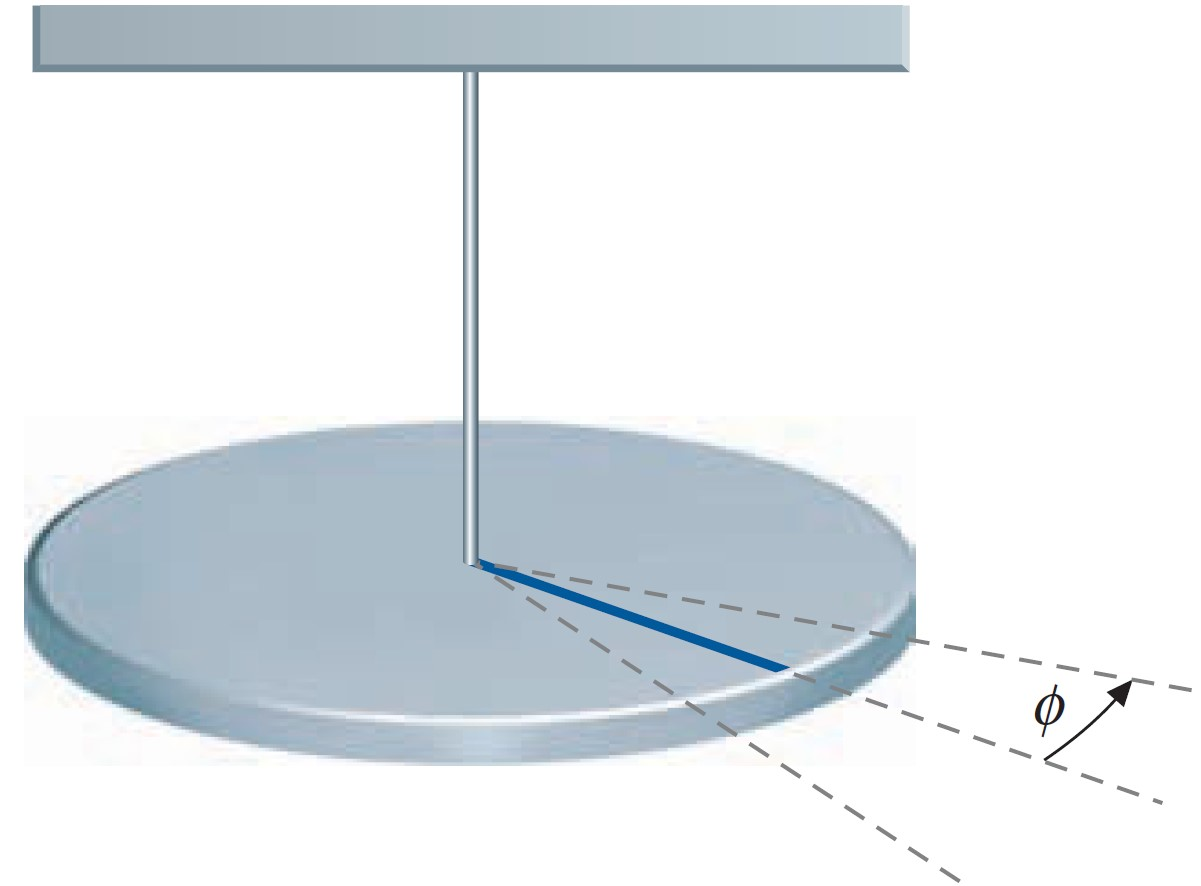
\includegraphics[width=3cm]{Physics/1st/Waves_and_optics/Images/tors.jpg}
  %         \end{minipage}
  %   \item Pèndol físic:
  %         \begin{gather*}
  %           \tau=-MgD\sin\phi=I\alpha\implies\kappa=MgD\\
  %           \phi=\phi_0\cos(\omega t)\\
  %           \omega=\sqrt{\frac{MgD}{I}}
  %         \end{gather*}
  %         {\footnotesize on $D$ és la distància del centre de masses a l'eix de rotació.}\newline
  %         \begin{minipage}{\linewidth}
  %           \centering
  %           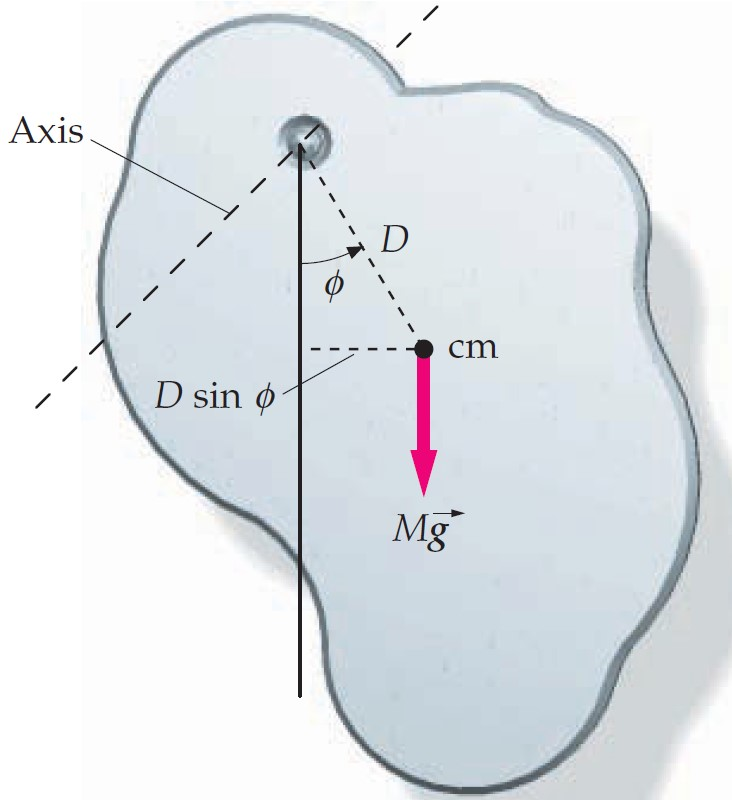
\includegraphics[width=3cm]{Physics/1st/Waves_and_optics/Images/fisic.jpg}
  %         \end{minipage}
  % \end{itemize}
  % Moviment harmònic esmorteït:
  % \begin{gather*}
  %   \Vec{F}_f=-\gamma\Vec{v}\qquad 2\beta=\frac{\gamma}{m}\\
  %   \omega_0=\sqrt{\frac{k}{m}}\quad\omega=\sqrt{\omega_0^2-\beta^2}\\
  %   \begin{multlined}
  %     \frac{d^2x}{dt^2}+\frac{\gamma}{m}\frac{dx}{dt}+\frac{k}{m}x=\\=\frac{d^2x}{dt^2}+2\beta\frac{dx}{dt}+\omega_0^2x=0
  %   \end{multlined}\\
  %   \implies\lambda^2+2\beta\lambda+\omega_0^2=0
  % \end{gather*}
  % {\footnotesize on $\Vec{F}_f$ és la força de fregament; $\gamma$, el coeficient de fregament ($[\gamma]=kg/s$); $\beta$, la constant d'esmorteïment ($[\beta]=s^{-1}$); $\omega_0$, la freqüència sense esmorteïment, i $\omega$, la freqüència. En l'última equació hem fet servir que $x=e^{\lambda t}$ per ser una equació diferencial homogènia de segon ordre.}
  % \begin{itemize}
  %   \item Sub-esmorteït ($\beta^2-\omega_0^2<0$):
  %         \begin{gather*}
  %           \lambda=-\beta\pm i\omega\\
  %           T=\frac{4\pi m}{\sqrt{4mk-\gamma^2}}\\
  %           x=A_0e^{-\beta t}\cos(\omega t+\phi_0)\\
  %           A_n=A_0e^{-2\beta Tn}
  %         \end{gather*} {\footnotesize on $A_n$ és l'amplitud de l'$n$-èssima oscil·lació.}\newline
  %         Energia d'oscil·lació i potència perduda:
  %         \begin{gather*}
  %           E\propto A^2\propto (e^{-\beta t})^2\\
  %           E=\frac{1}{2}m\omega^2A_0^2e^{-2\beta t}=E_0e^{-2\beta t}\\
  %           P=\frac{dE}{dt}=Fv=-\gamma v^2
  %         \end{gather*}
  %         Factor de qualitat $Q$:
  %         \begin{gather*}
  %           Q=\frac{\omega_0}{2\beta}\\
  %           Q=\frac{2\pi}{(|\Delta E|/E)_{\text{cicle}}}\\
  %           \omega=\omega_0\sqrt{1-\frac{1}{4Q^2}}
  %         \end{gather*} {\footnotesize on $(|\Delta E|/E)_{\text{cicle}}$ és l'energia perduda per cicle.}\newline
  %         \begin{minipage}{\linewidth}
  %           \centering
  %           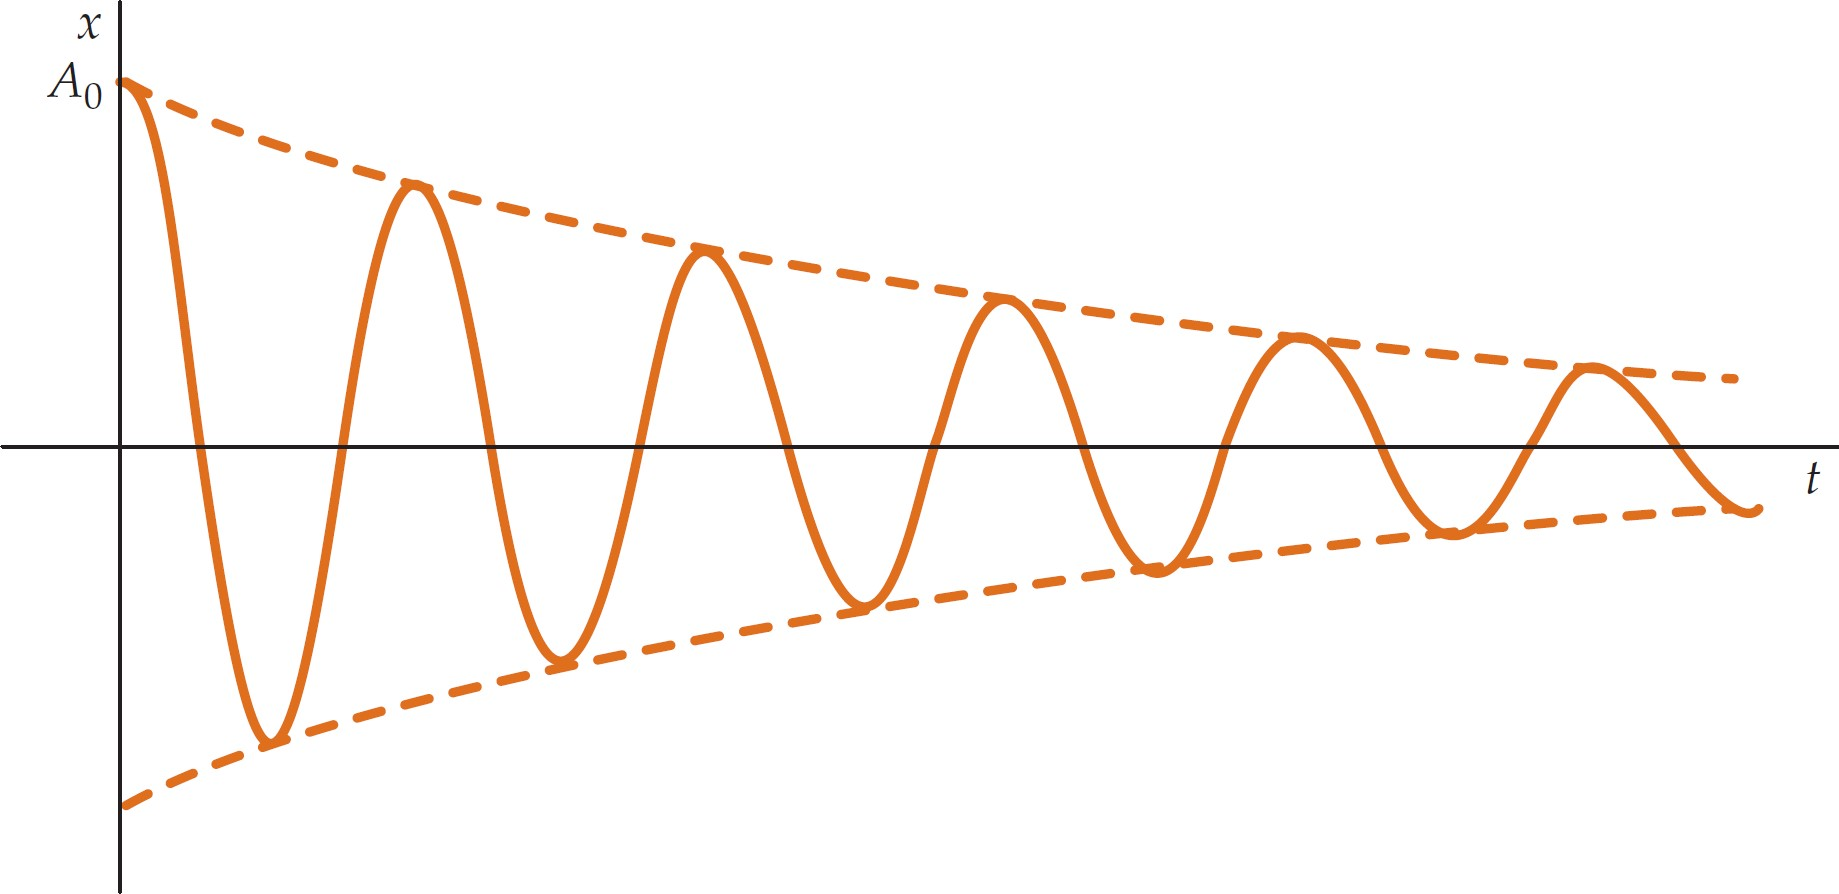
\includegraphics[width=\linewidth]{Physics/1st/Waves_and_optics/Images/udamp.jpg}
  %         \end{minipage}
  %   \item Esmorteïment crític ($\beta^2 -\omega_0^2=0$):
  %         \begin{gather*}
  %           \lambda=-\beta\\
  %           x(t)=(A_0+c_1t)e^{-\beta t}\\
  %           \gamma=\sqrt{4km}
  %         \end{gather*}
  %         {\footnotesize on $c_1$ és una constant.}
  %   \item Sobre-esmorteït ($\beta^2-\omega_0^2>0$):
  %         \begin{gather*}
  %           \lambda_1=-\beta+\sqrt{\beta^2-\omega_0^2}\\
  %           \lambda_2=-\beta-\sqrt{\beta^2-\omega_0^2}\\
  %           x(t)=c_1e^{-|\lambda_1|t}+c_2e^{-|\lambda_2|t}
  %         \end{gather*}
  %         {\footnotesize on $c_1$ i $c_2$ són constants.}\newline
  %         \begin{minipage}{\linewidth}
  %           \centering
  %           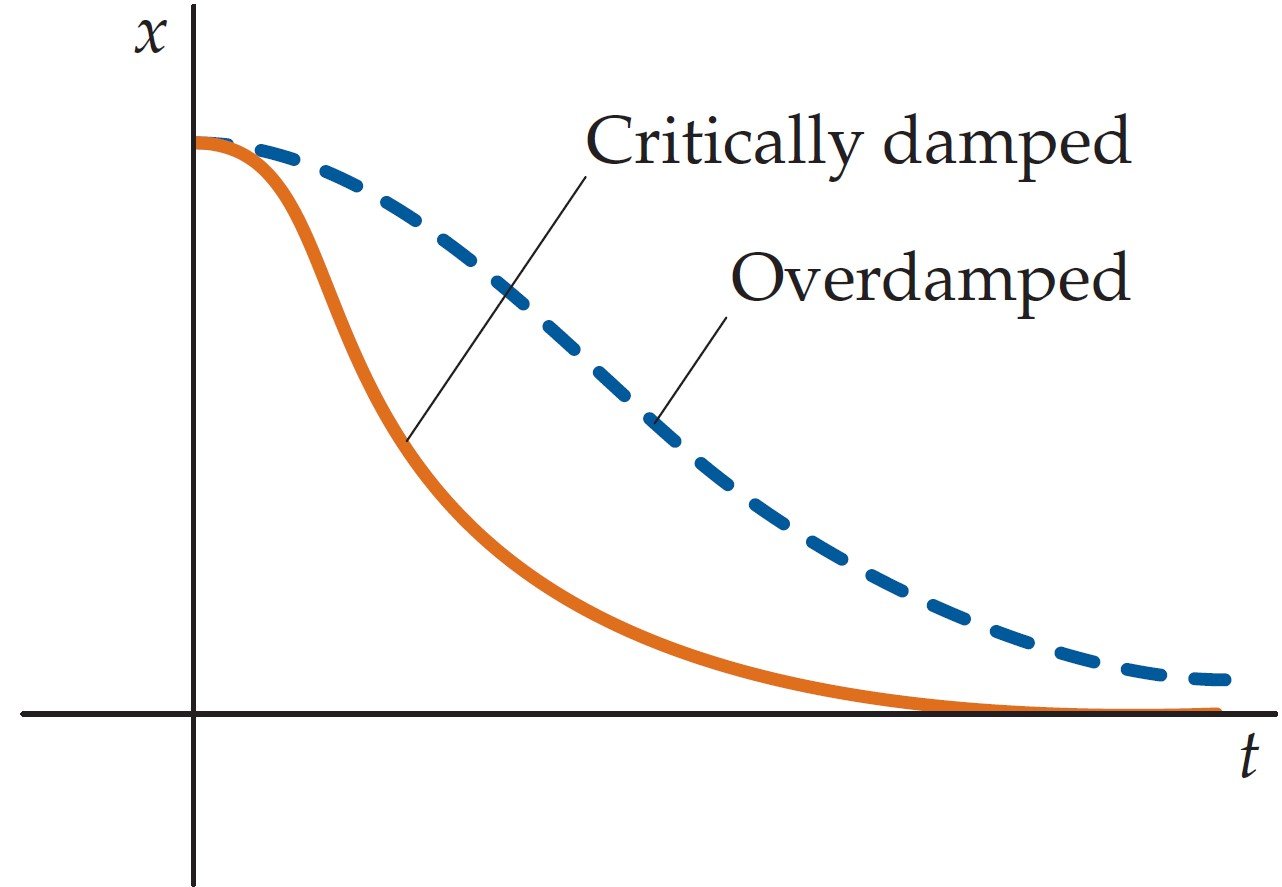
\includegraphics[width=\linewidth]{Physics/1st/Waves_and_optics/Images/cdamp.jpg}
  %         \end{minipage}
  % \end{itemize}
  % Oscil·lació reforçada:
  % \begin{gather*}
  %   \frac{d^2x}{dt^2}+\frac{\gamma}{m}\frac{dx}{dt}+\frac{k}{m}x=\frac{F_0}{m}\cos(\omega_{\text{ext}}t)\\
  %   x(t)=A\cos(\omega_\text{ext}t+\phi_0)\\
  %   A=\frac{F/m}{\sqrt{(\omega_{\text{ext}}^2-\omega_0^2)^2+4\beta^2\omega_\text{ext}^2}}\\
  %   \tan\phi_0=\frac{2\beta\omega_{\text{ext}}}{\omega_{\text{ext}}^2-\omega_0^2}
  % \end{gather*}
  % {\footnotesize Les solucions de l'equació diferencial estan formades per solucions del tipus $X(t)=y(t)+x(t)$, on $y(t)$ és la part transitòria (que s'anul·a passat un cert temps i és semblant a les condicions d'esmorteïment) i $x(t)$ és la part estacionària (s'aporta al sistema una energia igual a la que es dissipa).}\newline
  % Ressonància:
  % \begin{gather*}
  %   \omega_{\text{ext}}\to\omega_0\implies\tan\phi_0\to\infty\implies\phi_0\to\frac{\pi}{2}\\
  %   A=\frac{F_0/m}{2\beta\omega_0}
  % \end{gather*}
  % Energia de l'oscil·lació reforçada:
  % \begin{multline*}
  %   E(t)=\frac{A^2}{2}\left(m\omega^2\sin^2(\omega_{\text{ext}}t+\phi_0)+\right.\\\left.+k^2\cos^2(\omega_{\text{ext}}t+\phi_0)\right)\\
  %   \langle E\rangle=\frac{1}{T}\int_0^TE(t)dt=A^2\frac{m\omega_{\text{ext}}^2+k^2}{4}
  % \end{multline*}
  % Potència de l'oscil·lació reforçada:
  % \begin{align*}
  %    & P(t)=-\gamma v^2=-\gamma A^2\omega_{\text{ext}}^2\cos^2\left(\frac{2\pi}{T}t+\phi_0\right) \\
  %   \begin{split}
  %     &\langle P\rangle_{\text{diss}}=\frac{1}{T}\int_0^TP(t)dt=\\&\qquad\qquad\qquad=-\frac{\beta\omega_\text{ext}^2F_0^2/m}{(\omega_\text{ext}^2-\omega_0^2)^2+4\beta^2\omega_\text{ext}^2}
  %   \end{split}
  % \end{align*}
  % Amplada de ressonància per esmorteïment dèbil:
  % $$\frac{\Delta\omega}{\omega_0}=\frac{1}{Q}$$
  % \begin{minipage}{\linewidth}
  %   \centering
  %   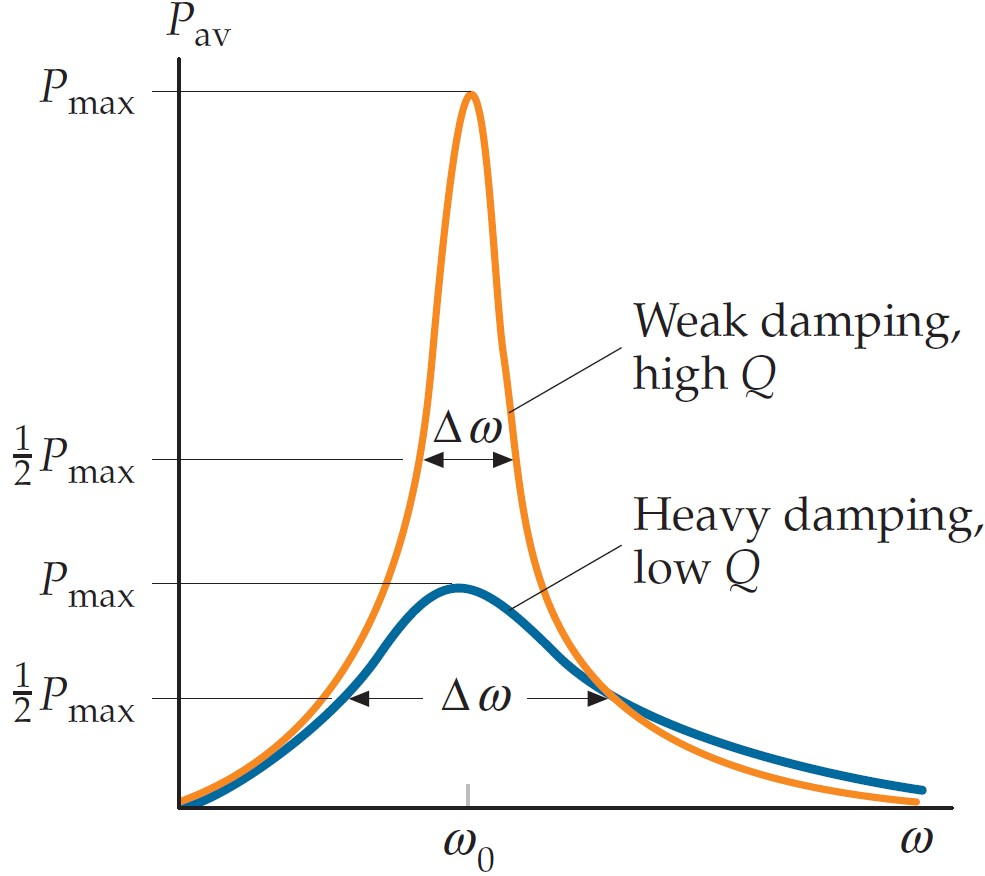
\includegraphics[width=\linewidth]{Physics/1st/Waves_and_optics/Images/q.jpg}
  % \end{minipage}
  % Donades dues oscil·lacions harmòniques amb amplituds $A_1$ i $A_2$, freqüències d'oscil·lació $\omega_1$ i $\omega_2$ i angles de fase $\phi_1$ i $\phi_2$, podem tenir les següents interferències:
  % \begin{itemize}
  %   \item Interferència amb $\omega_1=\omega_2$:
  %         \begin{gather*}
  %           A_T^2=A_1^2+A_2^2+2A_1A_2\cos(\Delta\phi)\\
  %           \tan\phi_T=\frac{A_1\sin\phi_1+A_2\sin\phi_2}{A_1\cos\phi_1+A_2\cos\phi_2}
  %         \end{gather*}
  %   \item Interferència amb $A_1=A_2$: \begin{multline*}
  %           x_T(t)=2A\sin\left(\frac{\omega_1+\omega_2}{2}t\right)\cdot\\\cdot\cos\left(\frac{\omega_2-\omega_1}{2}t\right)
  %         \end{multline*}
  %   \item Interferència de $n$ oscil·lacions d'igual amplitud i freqüència i fases diferents ($\phi_n=n\phi_0$):
  %         \begin{gather*}
  %           x_T(t)=A_T\cos(\omega t+\theta)\\
  %           A_T=A\frac{\sin(n\phi/2)}{\sin\phi/2}\quad\theta=(n-1)\frac{\phi}{2}
  %         \end{gather*}
  % \end{itemize}
  % Associació de motlles:
  % \begin{itemize}
  %   \item en sèrie: $$\frac{1}{k_T}=\sum_i\frac{1}{k_i}$$
  %   \item en paral·lel: $$k_T=\sum_ik_i$$
  % \end{itemize}
  % \subsection{Ones}
  % Equació d'ona (corda): $$\frac{T}{\lambda}\frac{\partial^2y}{\partial x^2}=\frac{\partial^2 y}{\partial t^2}$$ {\footnotesize on $T$ és la tensió de la corda i $\lambda$ la densitat lineal d'aquesta.}\newline
  % Ona viatgera: $$\frac{\partial^2f}{\partial t^2}=v^2\frac{\partial^2f}{\partial x^2}$$
  % Velocitat de les ones:
  % \begin{itemize}
  %   \item en un corda: $$v=\sqrt{\frac{T}{\lambda}}$$
  %   \item d'aigua: $$v=\sqrt{gh}$$ {\footnotesize on $h$ és la profunditat.}
  % \end{itemize}
  % Transformada de Fourier de funcions pe\-riò\-di\-ques i no periòdiques:
  % \begin{gather*}
  %   f(x,t)=\sum_{n=1}^\infty A_n\sin(\omega_nt\pm k_nx_n)\\
  %   f(x,t)=\int A(x)\sin(\omega t\pm kx)dx
  % \end{gather*}
  % Equació d'ona harmònica:
  % \begin{gather*}
  %   y(x,t)=A\sin(\omega t\pm kx+\phi_0)
  % \end{gather*}
  % {\footnotesize on els signes $\pm$ fan referència al sentit del moviment ($-x$ o $+x$). En les equacions següents emprarem únicament el signe $-$.}\newline
  % Relacions:
  % \begin{gather*}
  %   \omega=\frac{2\pi}{T}=2\pi f\qquad v=\frac{\lambda}{T}=\lambda f\\
  %   k=\frac{2\pi}{\lambda}=\frac{\omega}{v}\qquad 2\pi=\frac{\Delta x}{vT}
  % \end{gather*}
  % Velocitat i acceleració:
  % \begin{gather*}
  %   v(x,t)=A\omega\cos(\omega t-kx+\phi_0)\\
  %   a(x,t)=-A\omega^2\sin(\omega t-kx+\phi_0)
  % \end{gather*}
  % Energia i potència:
  % \begin{gather*}
  %   E_m=\frac{\omega^2A^2\lambda vt}{2}=\frac{\omega^2A^2\lambda x}{2}\\
  %   P_m=\frac{dE}{dt}=\frac{\omega^2A^2\lambda v}{2}\\
  %   P=\omega^2A^2\lambda v\cos^2(\omega t-kx)
  % \end{gather*} {\footnotesize on $\lambda$ és la densitat lineal de l'objecte generador d'ones (per exemple, una corda).}\newline
  % Energia per unitat de volum $\eta$:
  % $$\eta=\frac{\rho\omega^2A^2}{2}$$
  % Superposició:
  % \begin{itemize}
  %   \item Diferent fase:
  %         \begin{gather*}
  %           y_1=A\sin(\omega t- kx)\\
  %           y_2=A\sin(\omega t- kx+\phi_0)\\
  %           \begin{split}
  %             y_3=y_1+y_2=\qquad\qquad\qquad\qquad\\=2A\sin\left(\omega t-kx+\frac{\phi_0}{2}\right)\cos\left(\frac{\phi_0}{2}\right)
  %           \end{split}\\
  %           \text{Desfase (destructiva): }\phi_0=\pi+2\pi k\\
  %           \text{Fase (constructiva): }\phi_0=2\pi k
  %         \end{gather*}
  %   \item Diferent posició:
  %         \begin{gather*}
  %           y_1=A\sin(\omega t- kx_1)\\
  %           y_2=A\sin(\omega t- kx_2+\phi_0)\\
  %           \begin{split}
  %             y_3=2A\cos\left(k\frac{x_2-x_1}{2}\right)\sin\bigg(\omega t-\\\left.-k\frac{x_2+x_1}{2}\right)
  %           \end{split}\\
  %           \text{Desfase (destr.): }\phi_0=(2n+1)\pi k\\
  %           \text{Fase (constr.): }\phi_0=2\pi nk
  %         \end{gather*}
  %   \item Diferent freqüència (batiments):\newline
  %         Considerem dues ones amb equacions: $$y_i(x,t)=A\sin(\omega_it-k_ix)$$ {\footnotesize on $i=1,2$.}\newline Com a ona resultant tenim:
  %         \begin{multline*}
  %           y_3=y_1+y_2=\\=2A\cos(\omega_mt-k_mx)\sin(\omega_pt-k_px)
  %         \end{multline*}{\footnotesize on $\omega_m:=(\omega_1-\omega_2)/2$ és la freqüència de modulació; $k_m:=(k_1-k_2)/2$, el nombre d'ona de modulació; $\omega_p:=(\omega_1+\omega_2)/2$, la freqüència de propagació, i $k_p:=(k_1+k_2)/2$, el nombre d'ona de propagació.}\newline
  %         Si suposem $\omega_1\approx\omega_2:=\omega$ i $k_1\approx k_2:=k$:\newline
  %         Velocitat d'ona modulada (ràpida): $$v_p=\frac{\omega_1+\omega_2}{k_1+k_2}\approx\frac{\omega}{k}=v_{\text{fase}}$$
  %         Velocitat d'ona moduladora (de grup):
  %         $$v_g=\frac{d\omega}{dk}=\frac{d(v_pk)}{dk}=v\left(1-\frac{k}{n}\frac{dn}{dk}\right)$$
  %         {\footnotesize on hem suposat que $v_p=c/n(k)$. Aquests fenòmens on $v(k)$ o $v(\omega)$ es coneixen com a dispersió cromàtica o dispersió.}\newline
  %         \begin{minipage}{\linewidth}
  %           \centering
  %           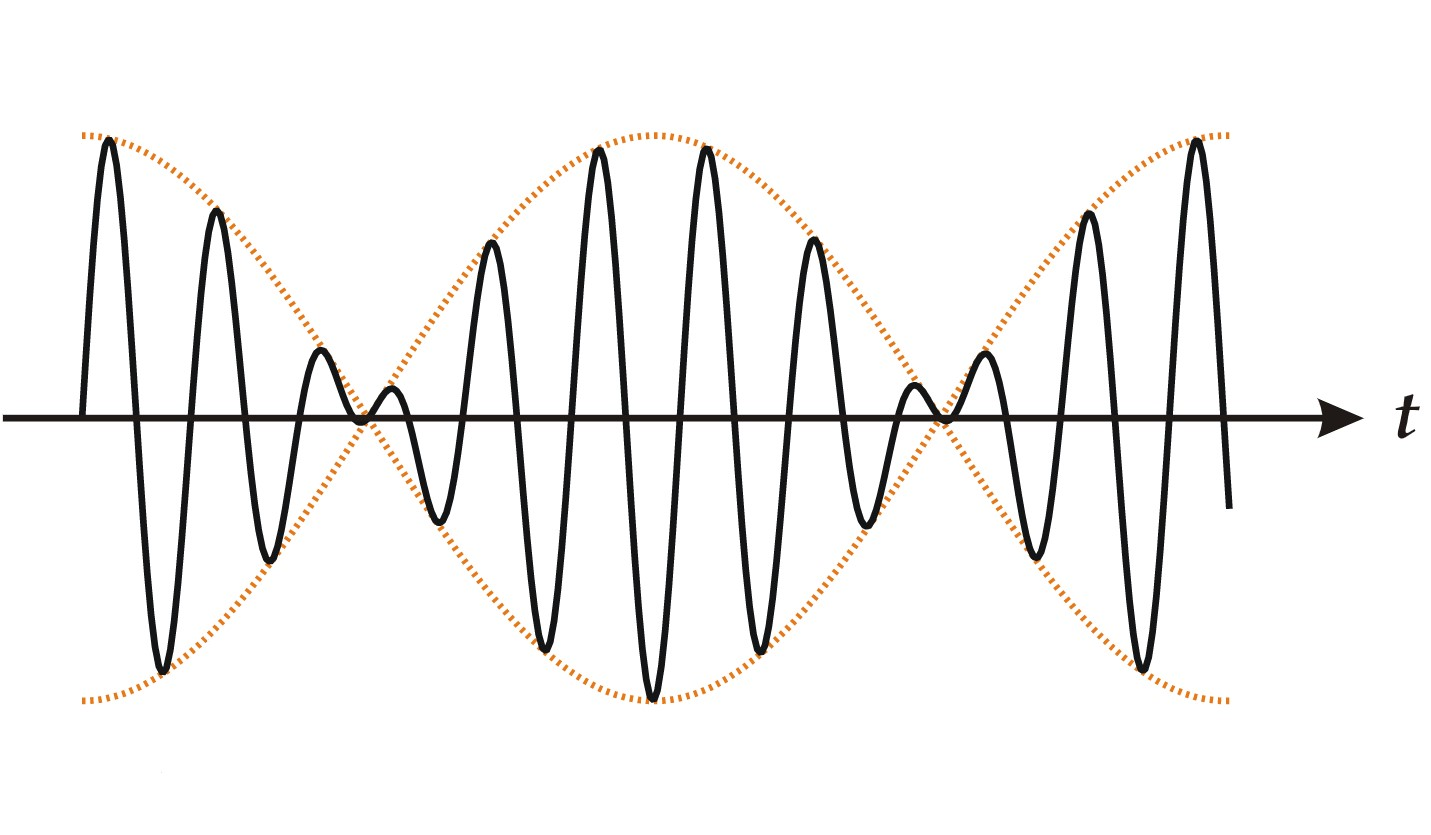
\includegraphics[width=5cm]{Physics/1st/Waves_and_optics/Images/beat.jpg}
  %           \captionof{figure}{Batiment. Aquí, $T_p=\frac{2\pi}{\omega_p}$ és el període de l'ona modulada i $T_m=\frac{2\pi}{\omega_m}$ és el període de l'ona moduladora. Com veiem a la figura: $T_m>T_p$.}
  %           \label{beat}
  %         \end{minipage}
  %         Intensitat:
  %         \begin{multline*}
  %           I=4A_0^2\cos^2\left(\omega_mt-k_mx\right)\cdot\\\cdot\sin^2\left(\omega_pt-k_px\right)
  %         \end{multline*}
  %   \item Ones estacionàries:\newline
  %         Considerem dues ones amb equacions:
  %         \begin{gather*}
  %           y_1=A_0\sin(\omega t-kx)\\
  %           y_2=A_0\sin(\omega t+kx+\phi_0)\\
  %           \begin{split}
  %             y_3=y_1+y_2=\qquad\qquad\\=2A_0\cos\left(kx+\frac{\phi_0}{2}\right)\sin\left(\omega t+\frac{\phi_0}{2}\right)
  %           \end{split}
  %         \end{gather*}
  %         Nodes: $$x=\frac{1}{k}\left[\frac{(2n+1)\pi}{2}-\frac{\phi_0}{2}\right]$$
  %         Ventres: $$x=\frac{1}{k}\left(n\pi-\frac{\phi_0}{2}\right)$$
  %         {\footnotesize on $n\in\ZZ$.}\newline En les ones estacionàries no hi ha propagació d'energia.\newline
  %         Tipus d'ones estacionàries ($n\in\NN$):
  %         \begin{itemize}
  %           \item Amb dos extrems fixos:
  %                 \begin{gather*}
  %                   \lambda_n=\frac{2L}{n}=\frac{\lambda_1}{n}\\
  %                   f_n=\frac{nv}{2L}=n\frac{1}{2L}\sqrt{T/\mu}=nf_1
  %                 \end{gather*}
  %           \item Amb un extrem fix i un de lliure:
  %                 \begin{gather*} \lambda_n=\frac{4}{2n-1}L=\frac{\lambda_1}{2n-1}\\
  %                   f_n=\frac{2n-1}{4L}\sqrt{T/\mu}=(2n-1)f_1
  %                 \end{gather*}
  %           \item Amb dos extrems lliures:
  %                 \begin{gather*}
  %                   \lambda_n=\frac{2L}{n}=\frac{\lambda_1}{n}\\
  %                   f_n=\frac{nv}{2L}=n\frac{1}{2L}\sqrt{T/\mu}=nf_1
  %                 \end{gather*}
  %         \end{itemize}
  %   \item Direccions perpendiculars (corbes de Lissajous):
  %         \begin{itemize}
  %           \item Mateixa freqüència:
  %                 Considerem dues ones amb equacions:
  %                 \begin{gather*}
  %                   \Vec{E}_1=A_1\sin(\omega t-kx)\Vec{e}_y\\
  %                   \Vec{E}_2=A_2\sin(\omega t-kx+\phi_0)\Vec{e}_z
  %                 \end{gather*}
  %                 Fent $x=0$:
  %                 $$\frac{z^2}{A_2^2}+\frac{y^2}{A_1^2}-\frac{2zy}{A_1A_2}\cos\phi_0=\sin^2\phi_0$$ {\footnotesize que és l'equació d'una el·lipse inscrita en un rectangle $A_1\times A_2$.}
  %           \item Diferents freqüències:\newline Suposant que les freqüències de les dues ones estan relacionades per:
  %                 $$\frac{\omega_1}{\omega_2}=\frac{a}{b}\in\QQ$$ D'aquesta manera combinant les dues equacions d'ona podem crear corbes com les que es mostren a la \cref{liss}.
  %         \end{itemize}
  %         \begin{minipage}{\linewidth}
  %           \centering
  %           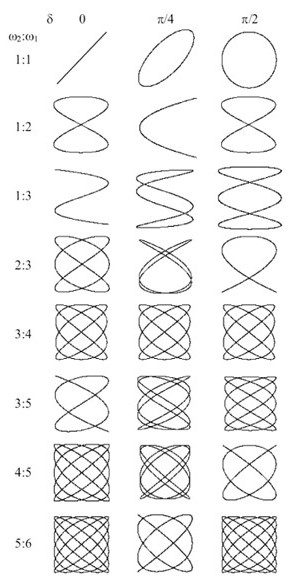
\includegraphics[width=4.3cm]{Physics/1st/Waves_and_optics/Images/liss.jpg}
  %           \captionof{figure}{Corbes de Lissajous. A les tres columnes es mostren les corbes seleccionant el desfasament $\delta$ que, d'esquerra a dreta, val $\delta=0$, $\delta=\pi/4$ i $\delta=\pi/2$. I a cada fila es mostra la relació $\omega_2:\omega_1=b:a$.}
  %           \label{liss}
  %         \end{minipage}
  % \end{itemize}
  % Anàlisi i síntesi harmòniques:\newline L'anàlisi de Fourier ens permet descompondre cadascuna d'aquestes funcions pe\-riò\-di\-ques com a combinació lineal de funcions harmòniques de diferents freqüències. D'altra banda, l'invers de l'anàlisi harmònica és la síntesi harmònica que consisteix en la construcció d'una funció periòdica a partir dels seus components harmònics.\newline
  % Difracció: Si l'ona que s'apropa a una es\-clet\-xa té una longitud d'ona similar a la longitud de l'obertura de l'escletxa, aleshores en tra\-ves\-sar aquesta l'escletxa els fronts d'ona es corben al voltant de l'obertura.\newline
  % \begin{minipage}{\linewidth}
  %   \centering
  %   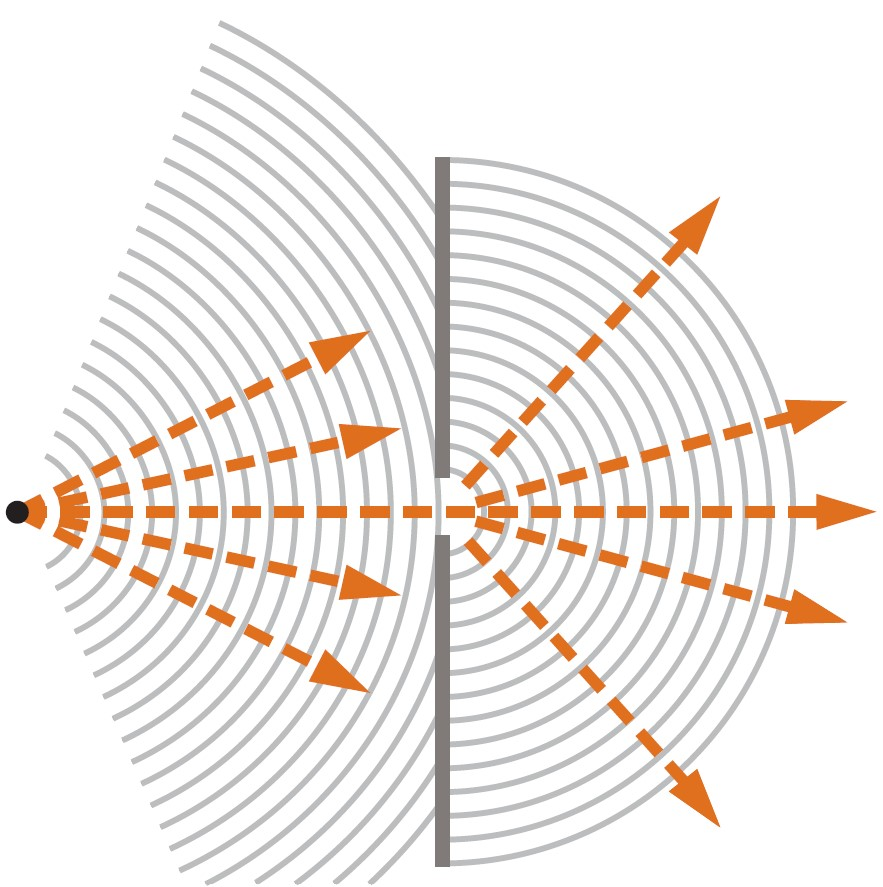
\includegraphics[width=2.95cm]{Physics/1st/Waves_and_optics/Images/diff.jpg}
  %   \captionof{figure}{Fenomen de difracció.}
  %   \label{diff}
  % \end{minipage}
  % Efecte Doppler:
  % \begin{equation*}
  %   \nu=\nu_0\frac{v-v_o\cos\beta}{v- v_s\cos\alpha}=\nu_0\frac{v-\Vec{v}_o\cdot\Vec{u}}{v- \Vec{v}_s\cdot\Vec{u}}\\
  % \end{equation*}
  % {\footnotesize on $v$ és la velocitat de l'ona; $v_o$, la del receptor, i $v_s$, la de l'emissor. $\nu_0$ és la freqüència de l'emissor i $\nu$ la del receptor. Els angles $\alpha$ i $\beta$ són els que formen respectivament l'emissor i el receptor respecte del vector unitari $u$ en la recta que els uneix.}\newline
  % \begin{minipage}{\linewidth}
  %   \centering
  %   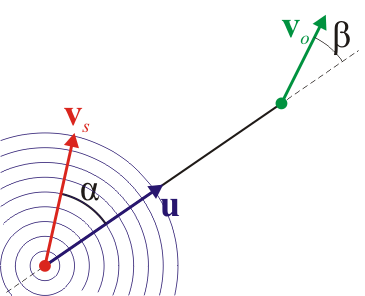
\includegraphics[width=4cm]{Physics/1st/Waves_and_optics/Images/dopp.png}
  %   \captionof{figure}{Cas general d'efecte Doppler no relativista.}
  %   \label{dopp}
  % \end{minipage}
  % Ones de xoc:
  % Angle ($\theta$) i nombre de Mach ($M$): $$\sin\theta=\frac{v}{u}\qquad M=\frac{u}{v}$$ {\footnotesize on s'ha emprat la notació de la \cref{xoc}.}\newline
  % \begin{minipage}{\linewidth}
  %   \centering
  %   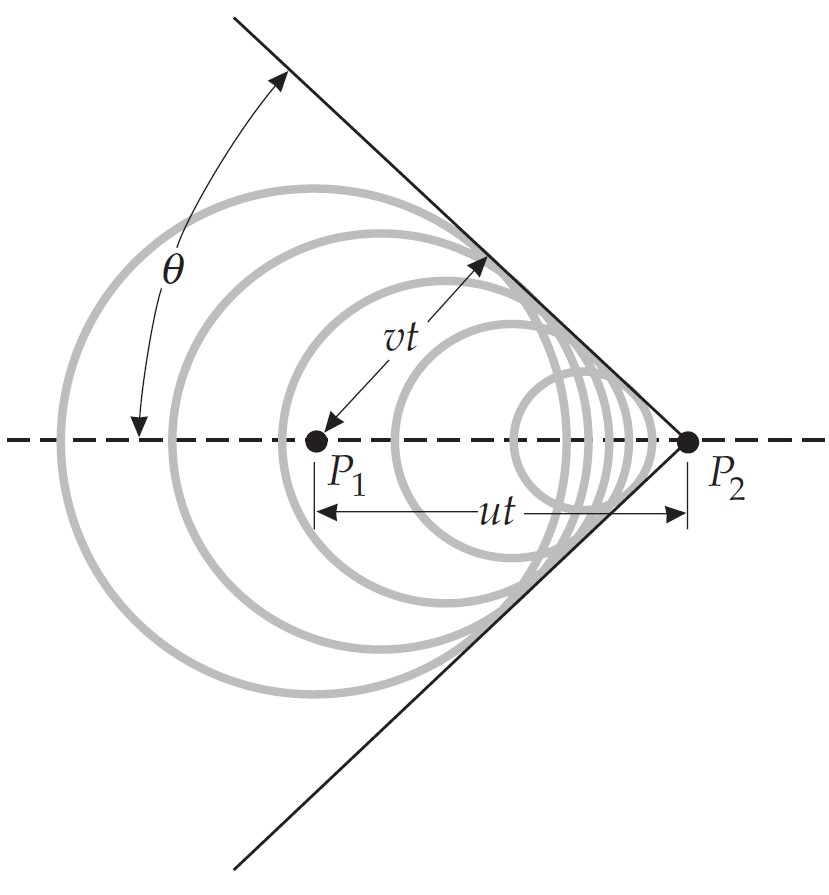
\includegraphics[width=4cm]{Physics/1st/Waves_and_optics/Images/onesdexoc.jpg}
  %   \captionof{figure}{Ones de xoc creades quan $u>v$, on $u$ és la velocitat de l'emissor i $v$ la velocitat de la font.}
  %   \label{xoc}
  % \end{minipage}
  % Trajectòria i pressió del so:
  % \begin{gather*}
  %   s(x,t)=s_0\sin\left(\omega t-kx\right)\\
  %   p(x,t)=p_0\cos\left(\omega t-kx\right)\\
  %   p_0=\rho\omega vs_0
  % \end{gather*}
  % {\footnotesize on $s(x,t)$ representa la trajectòria de les ones, $p(x,t)$, la pressió d'aquestes.}\newline
  % Velocitat ones sonores:
  % \begin{itemize}
  %   \item en un fluid: $$v=\sqrt{B/\rho}$$ {\footnotesize on $B=-\frac{\Delta P}{\Delta V/V}$ és el mòdul de com\-pres\-si\-bi\-li\-tat del fluid i $\rho$ és la densitat d'aquest.}
  %   \item en un sòlid:
  %         $$v=\sqrt{Y/\rho}$$ {\footnotesize on $Y$ és el mòdul de Young.}
  %   \item en un gas:
  %         $$v=\sqrt{\gamma RT/M}$$ {\footnotesize on $\gamma$ és el coeficient adiabàtic del gas; $M$, la massa molar d'aquest; $R=8,314\;J/(\text{mol}\cdot K)$, i $T$, la temperatura.}
  % \end{itemize}
  % Intensitat d'ones sonores:
  % \begin{gather*}
  %   I=\frac{P}{S}=\eta v=\frac{1}{2}\rho\omega^2s_0^2v v=\frac{1}{2}\frac{p_0^2}{\rho v}
  % \end{gather*}
  % Energia per unitat de volum $\eta$ d'ones sonores:
  % $$\eta=\frac{1}{2}\rho\omega^2s_0^2$$
  % Intensitat i decibels:
  % \begin{gather*}
  %   B=10\log_{10}\left(\frac{I}{I_0}\right)\\
  %   \text{llindar d'audició: }B= 0\;dB\\
  %   \text{llindar de dolor: }B= 120\;dB
  % \end{gather*}
  % {\footnotesize on $[B]=dB$ (decibels) i $I_0=10^{-12}\;W/m^2$.}
  % Relació intensitat$-$distància: $$\frac{I_1}{I_2}=\frac{P/S_1}{P/S_2}=\frac{S_2}{S_1}=\frac{r_2^2}{r_1^2}$$ {\footnotesize on $S_i$ és la superfície de l'esfera amb radi igual a la distància al focus emissor, $r_i$.}
  % \subsection{Òptica}
  % Dualitat ona-corpuscle:$$\lambda=\frac{h}{mv}\qquad\qquad E=hf$$
  % Interacció llum-matèria:\newline
  % \begin{minipage}{\linewidth}
  %   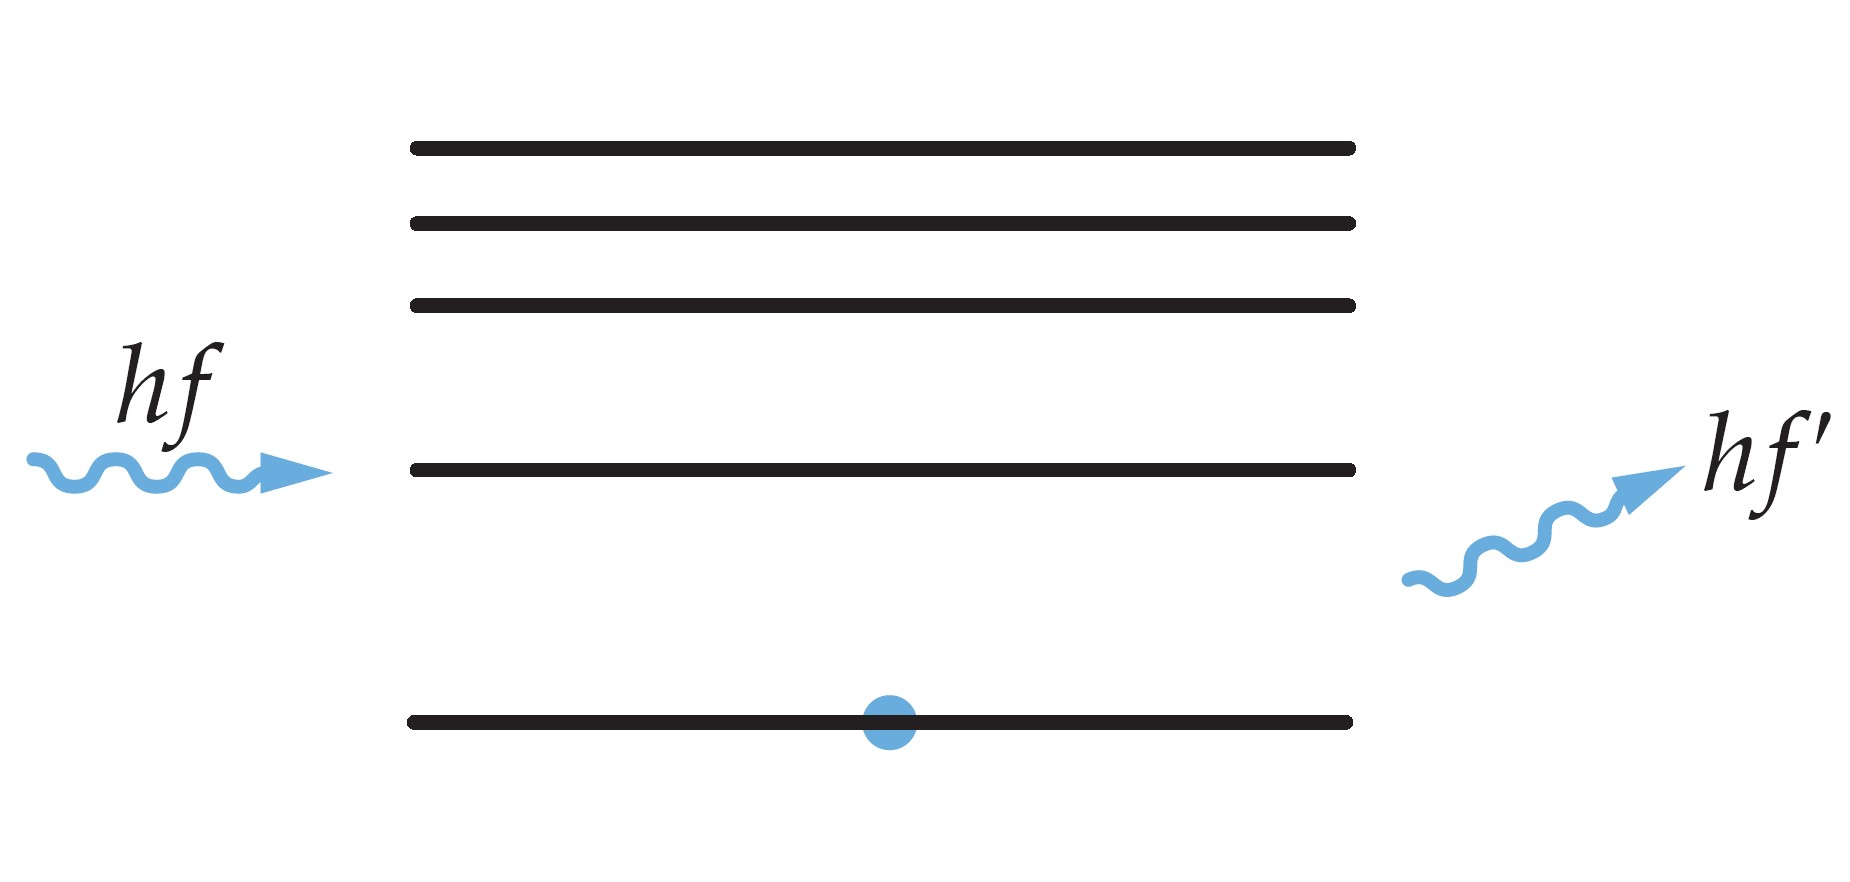
\includegraphics[width=\linewidth]{Physics/1st/Waves_and_optics/Images/elasticscatt.jpg}
  %   \captionof{figure}{Dispersió e\-làs\-ti\-ca.}
  % \end{minipage}
  % \begin{minipage}{\linewidth}
  %   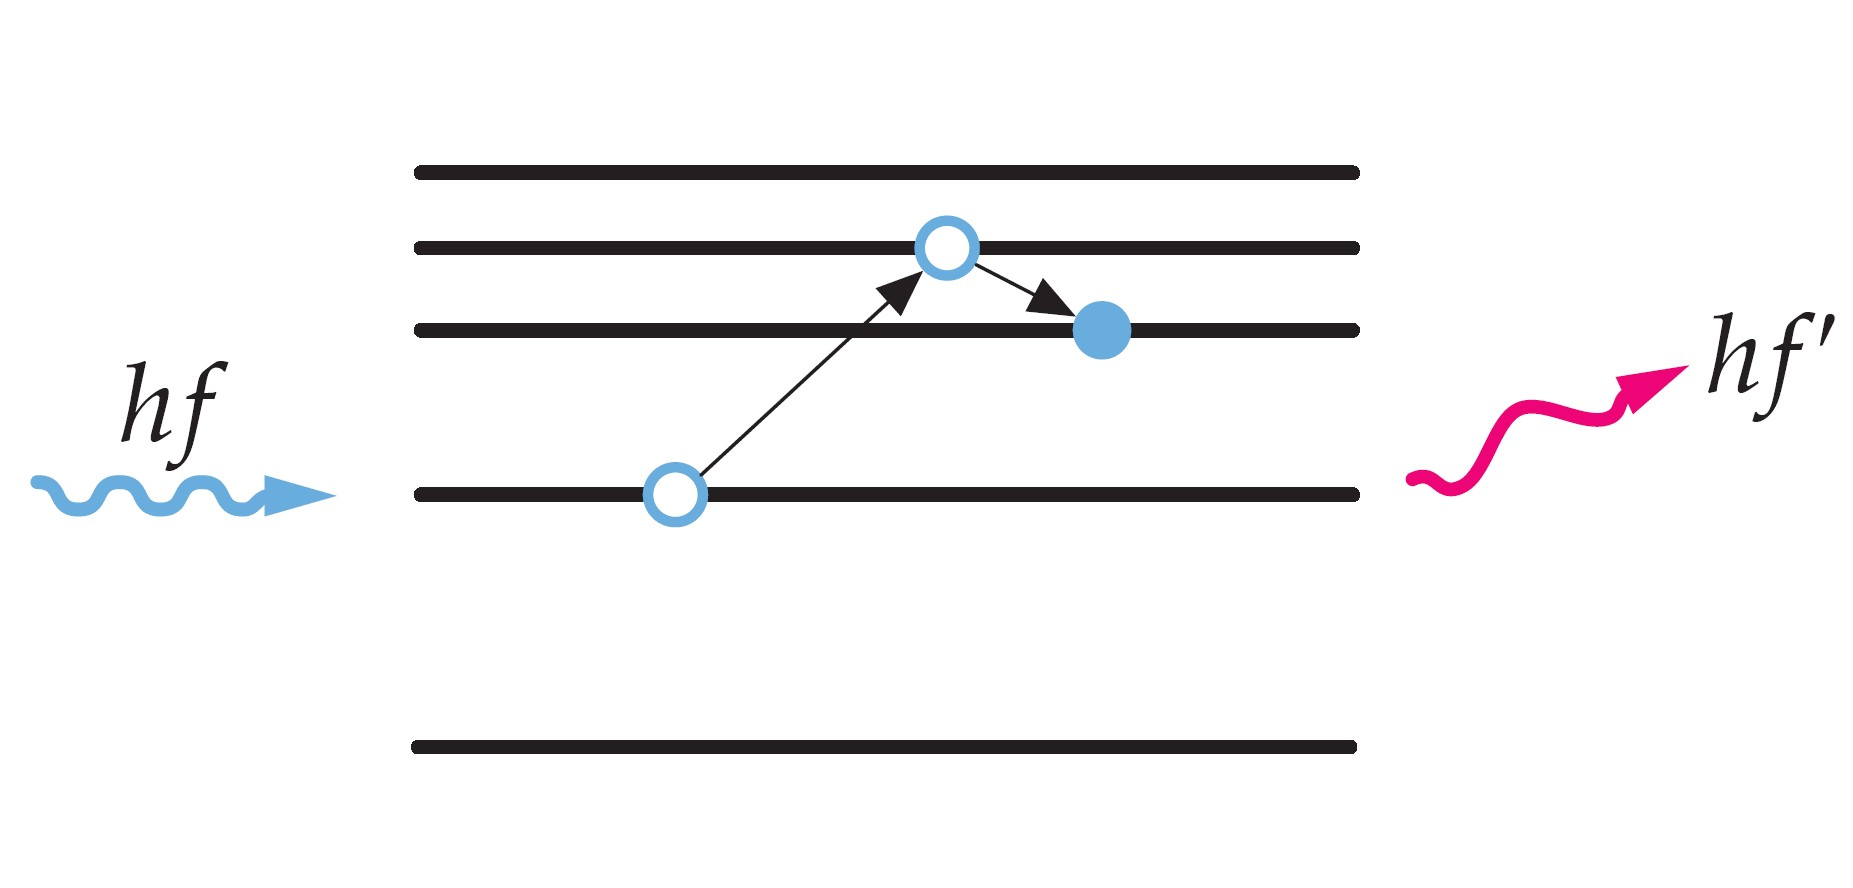
\includegraphics[width=\linewidth]{Physics/1st/Waves_and_optics/Images/StokesRamman.jpg}
  %   \captionof{figure}{Dispersió de Stokes Ramman.}
  % \end{minipage}
  % \begin{minipage}{\linewidth}
  %   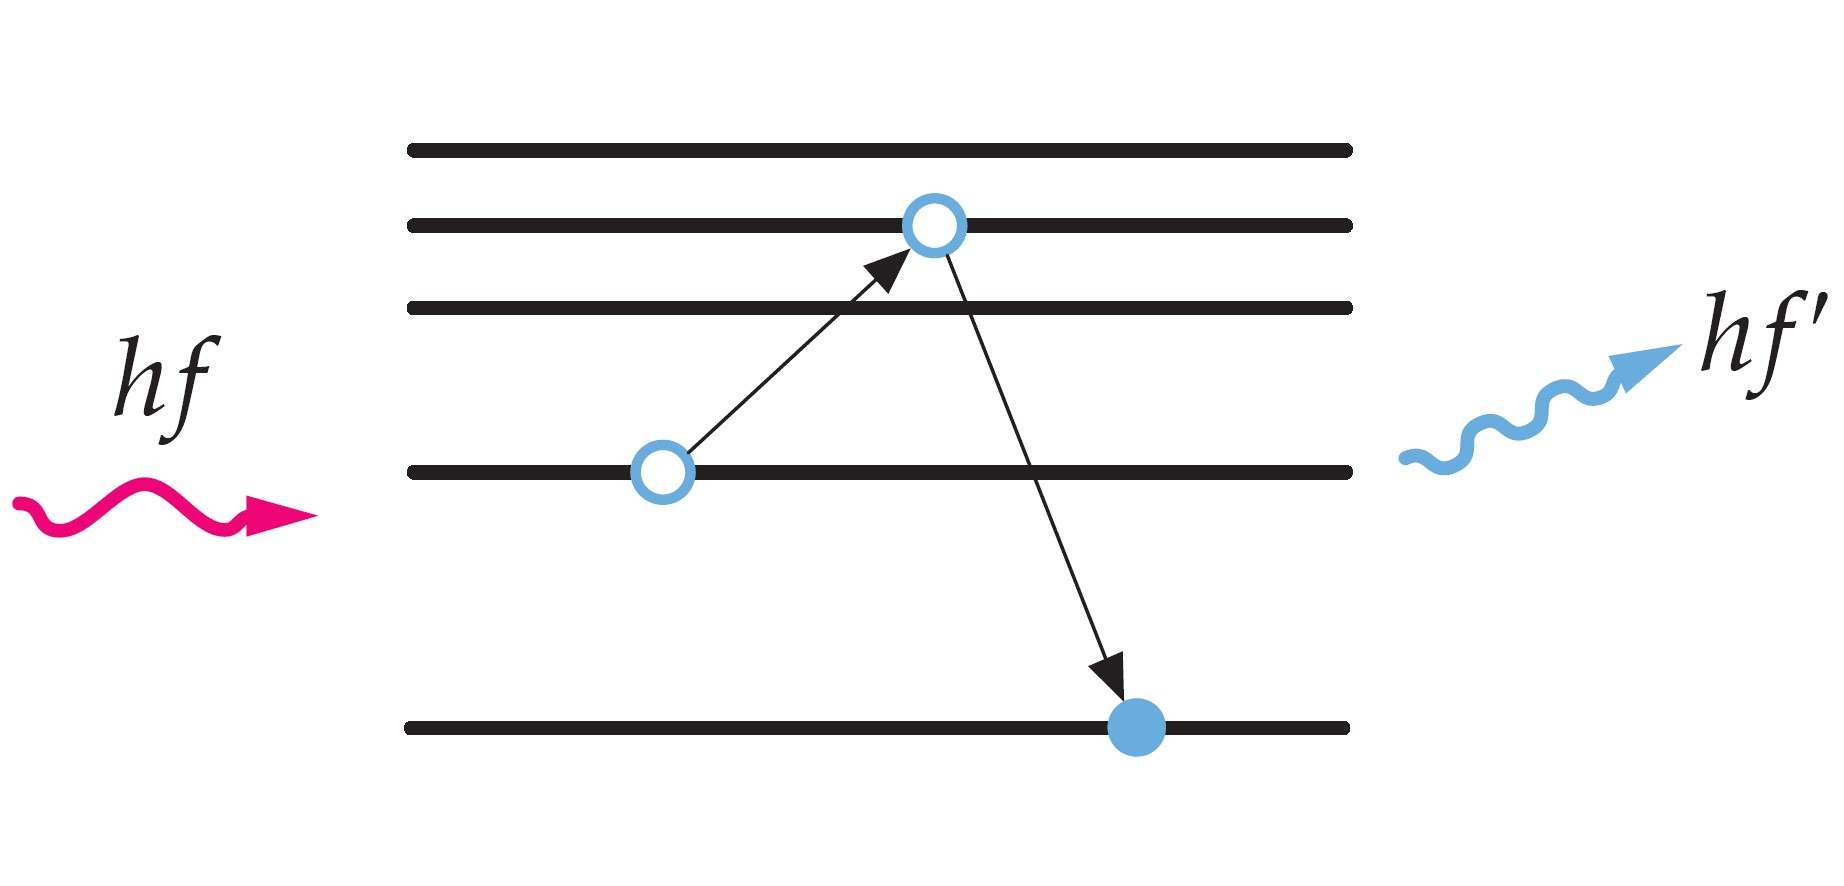
\includegraphics[width=\linewidth]{Physics/1st/Waves_and_optics/Images/AStokesRamman.jpg}
  %   \captionof{figure}{Dispersió an\-ti-Stokes Ramman.}
  % \end{minipage}
  % \begin{minipage}{\linewidth}
  %   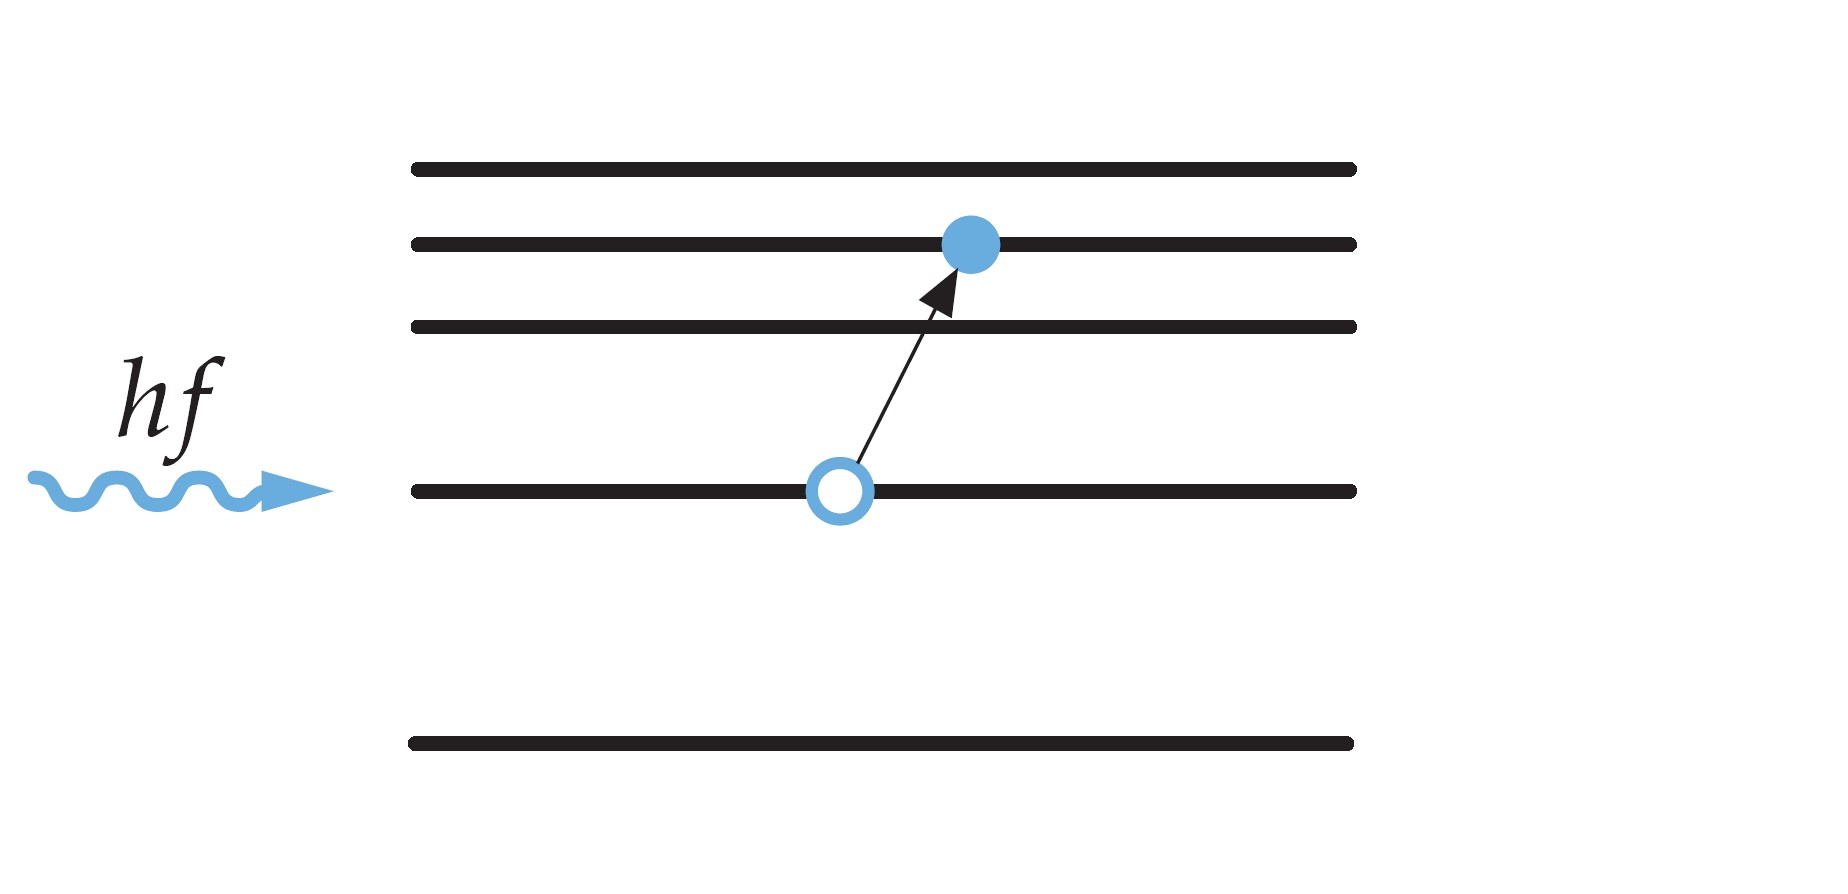
\includegraphics[width=\linewidth]{Physics/1st/Waves_and_optics/Images/Ressonance.jpg}
  %   \captionof{figure}{Absorció res\-so\-nant.}
  % \end{minipage}
  % \begin{minipage}{\linewidth}
  %   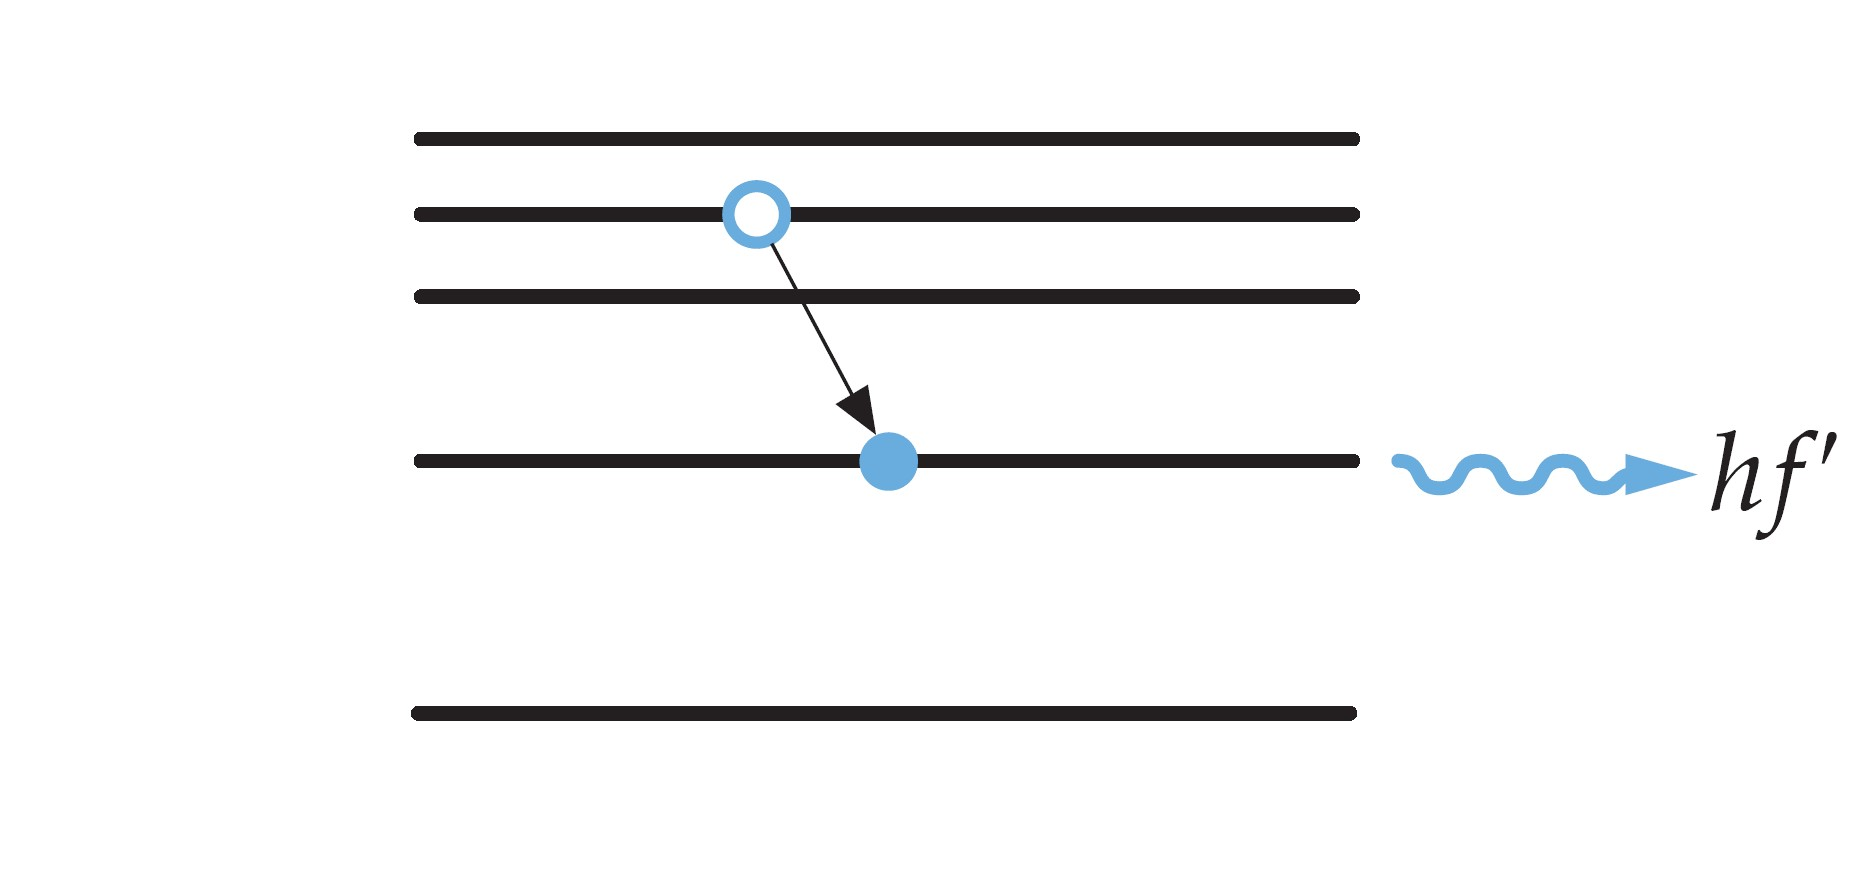
\includegraphics[width=\linewidth]{Physics/1st/Waves_and_optics/Images/spontaneous.jpg}
  %   \captionof{figure}{Emissió es\-pon\-tà\-ni\-a.}
  % \end{minipage}
  % \begin{minipage}{\linewidth}
  %   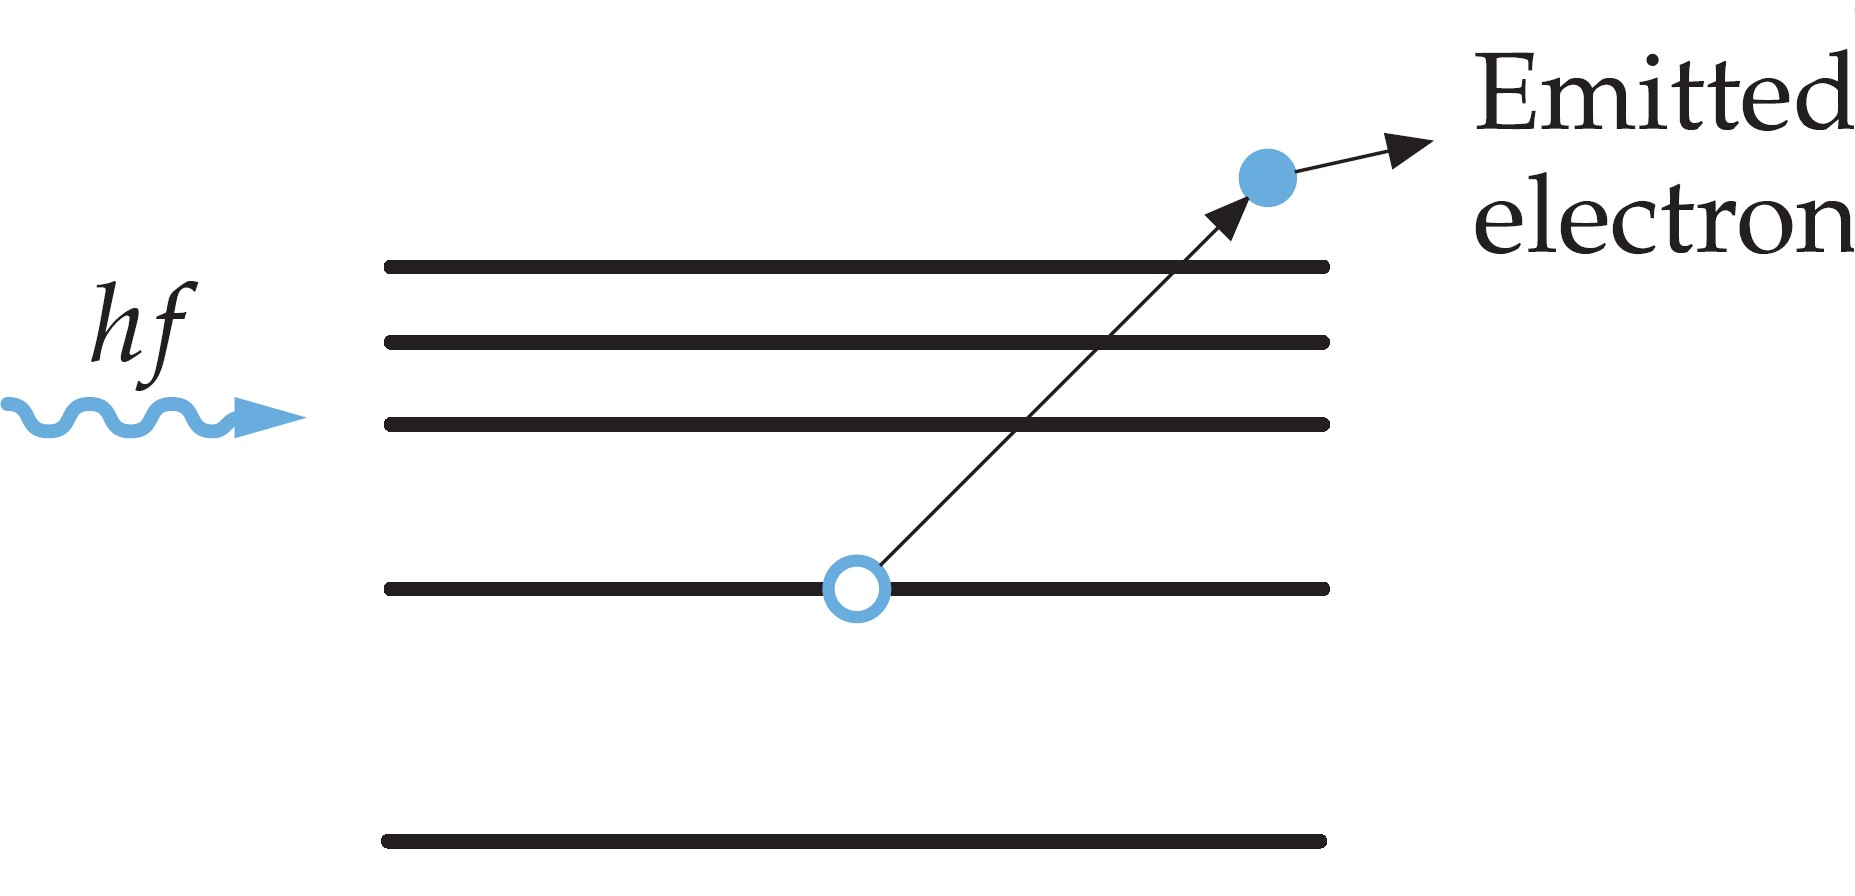
\includegraphics[width=\linewidth]{Physics/1st/Waves_and_optics/Images/photoelectric.jpg}
  %   \captionof{figure}{Efecte fo\-toe\-lèc\-tric.}
  % \end{minipage}
  % \begin{minipage}{\linewidth}
  %   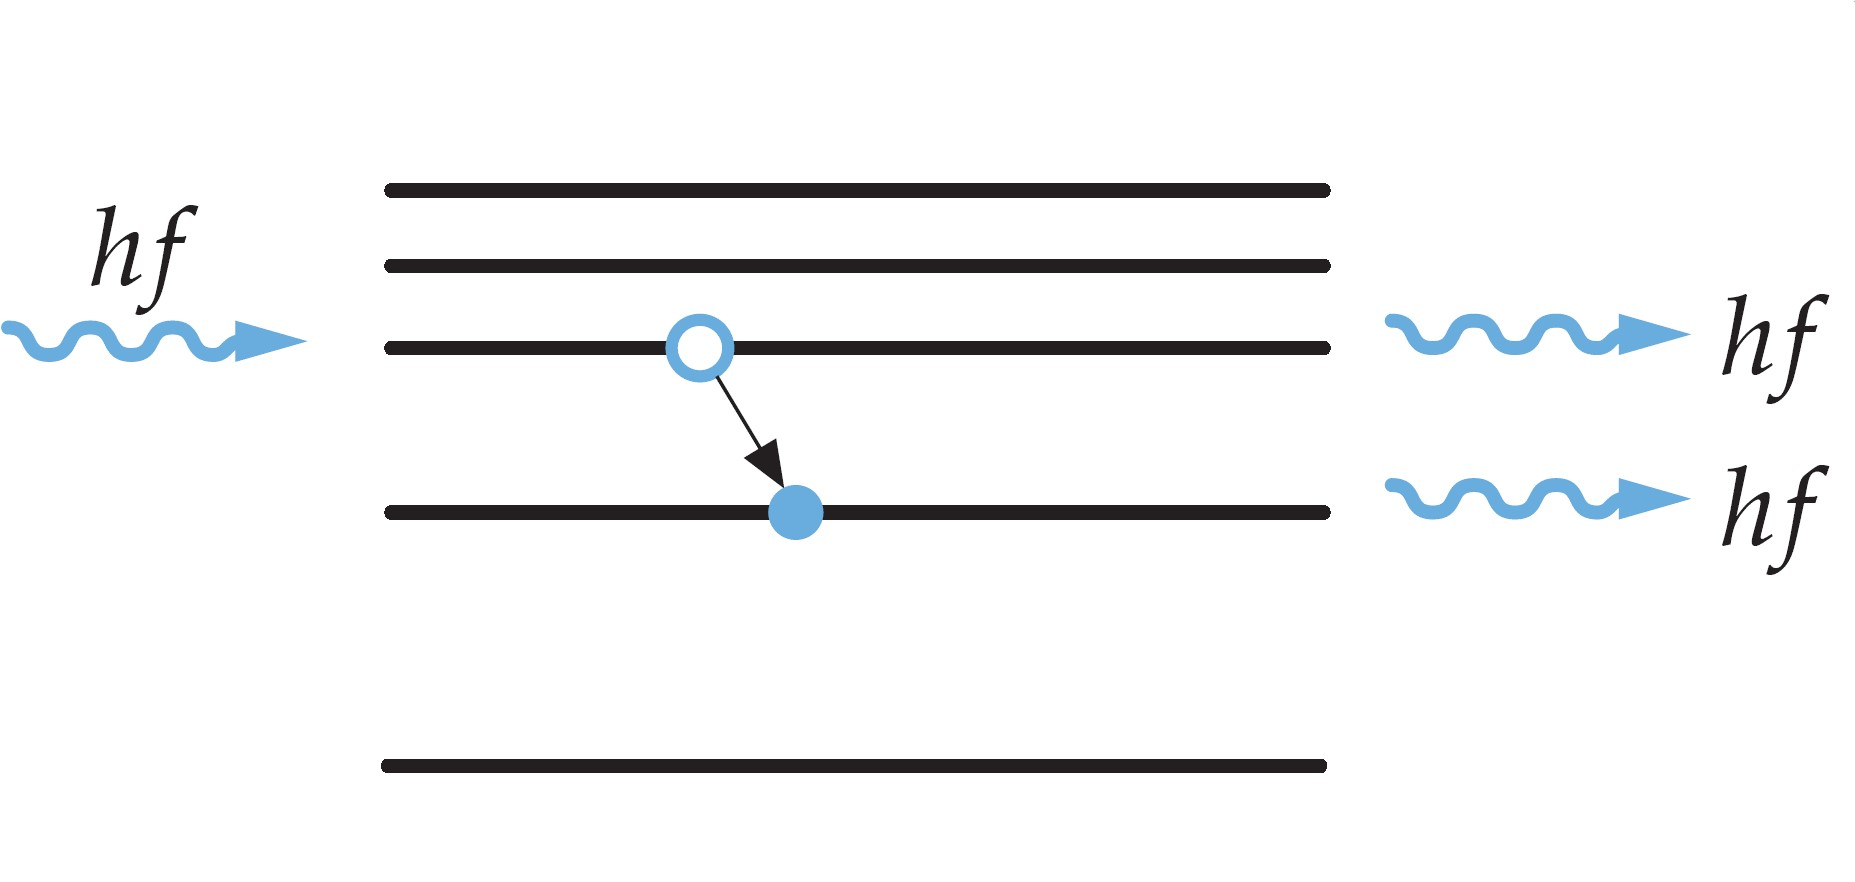
\includegraphics[width=\linewidth]{Physics/1st/Waves_and_optics/Images/stimulated.jpg}
  %   \captionof{figure}{Emissió es\-ti\-mu\-la\-da.}
  % \end{minipage}
  % \begin{minipage}{\linewidth}
  %   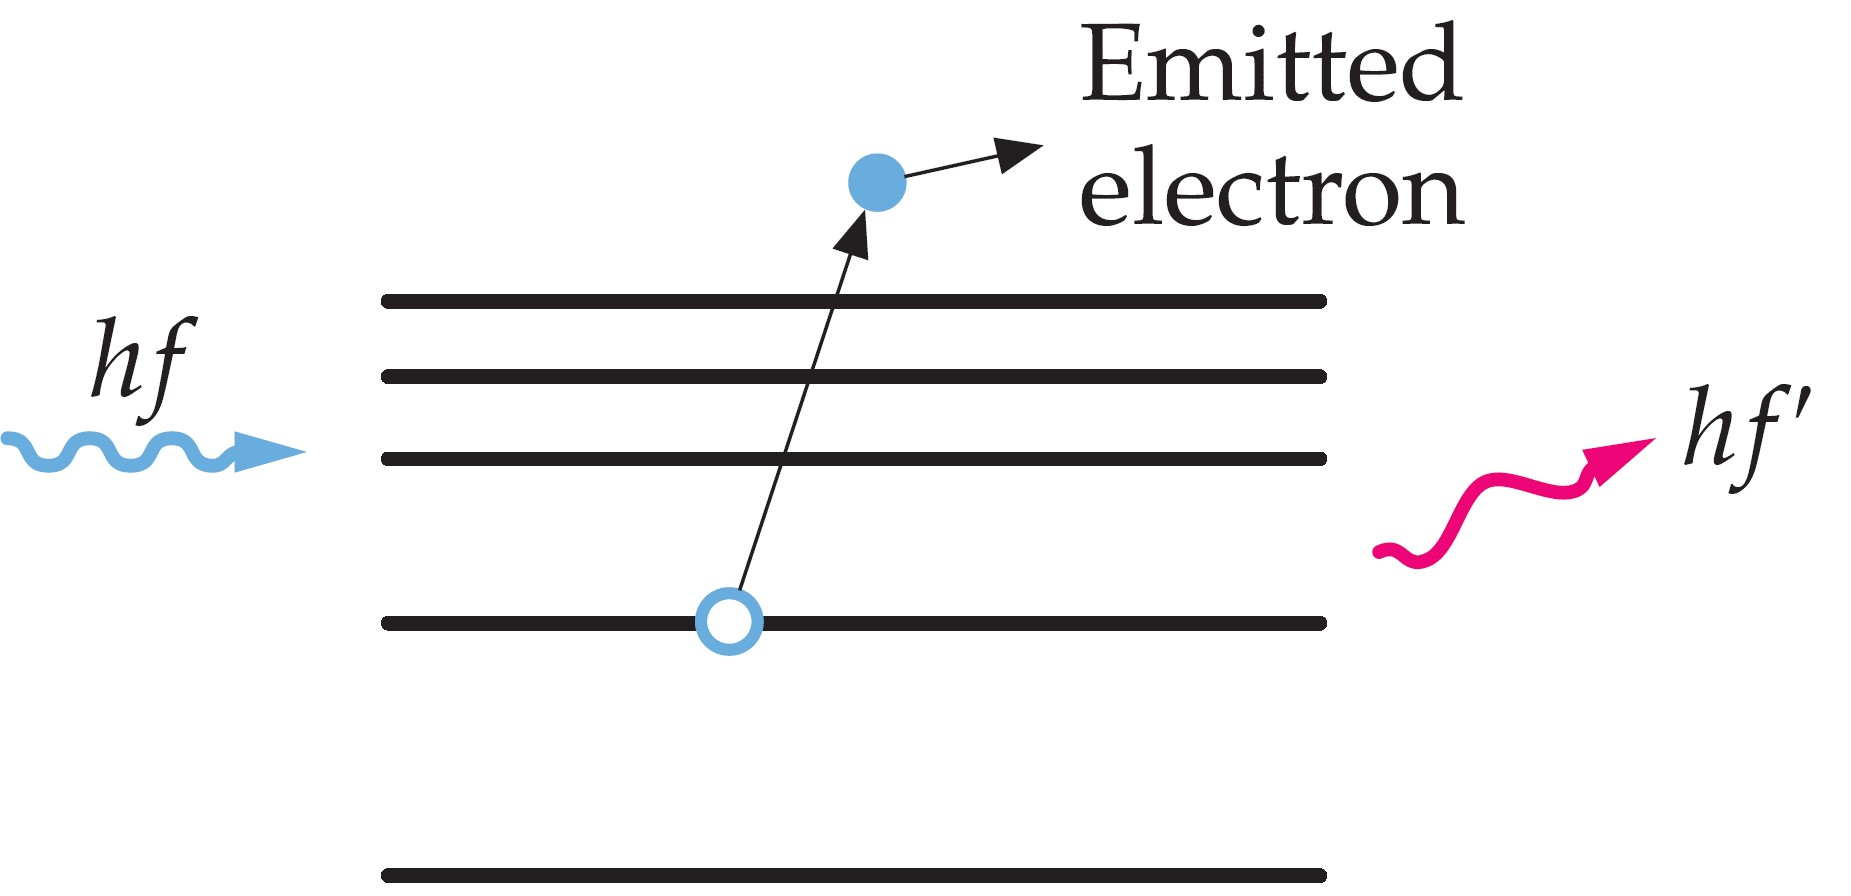
\includegraphics[width=\linewidth]{Physics/1st/Waves_and_optics/Images/compton.jpg}
  %   \captionof{figure}{Dispersió de Compton.}
  % \end{minipage}
  % Fluorescència i fosforescència: Si el procés absorció$-$emissió és quasi instantani (al vol\-tant de $ns$) tenim la fluorescència. Si el procés és molt més llarg (al voltant de $s$ o més), com que tenim nivells excitats quasi estacionaris, tenim el fenomen de la fosforescència.\newline
  % Fonts de llum:
  % \begin{itemize}
  %   \item convencionals: funcionen per emissió espontània. Ex: flama, sol, LED...
  %   \item làser (\textit{Light Amplification by Stimulated Emission of Radiation}): funcionen per emissió estimulada. Ne\-ces\-si\-ten un medi actiu (que emetrà la llum) que també s’ha d’excitar. En a\-quest medi cal aplicar una inversió de població (més àtoms excitats que en l’estat fonamental) i per això es necessita un sistema que aporti energia als àtoms anomenat sistema de bombeig. Finalment, també cal que hi hagi més emissió estimulada que espontània i això s’obté tenint molta llum atrapada, la qual cosa s’aconsegueix amb una estructura de dos miralls a\-li\-ne\-ats, a\-no\-me\-na\-da cavitat.
  % \end{itemize}
  % Principi de Huygens: Cada punt d’un front d’ones es pot considerar emissor d’ones esfèriques secundàries que avancen a la mateixa velocitat i freqüència que l’ona primària. El nou front d’ona (al cap d’un cert temps) és l’envoltant (corba tangent a totes les ones esfèriques) de les ones secundàries.\newline
  % Principi de Fresnel: El nou front d’ones al cap d’un cert temps és la superposició de les ones secundàries.\newline
  % Principi de Fermat: La trajectòria que se\-gueix la llum per anar d’un punt $A$ a un punt $B$ és aquella que fa que el temps transcorregut sigui mínim.\newline
  % Índex de refracció del material: $$n\equiv\frac{c}{v}$$
  % Llei de reflexió: $$\theta_1=\theta_1'$$
  % Llei de refracció (Snell): $$n_1\sin\theta_1=n_2\sin\theta_2$$
  % Reflexió especular i reflexió difosa:\newline
  % \begin{minipage}{\linewidth}
  %   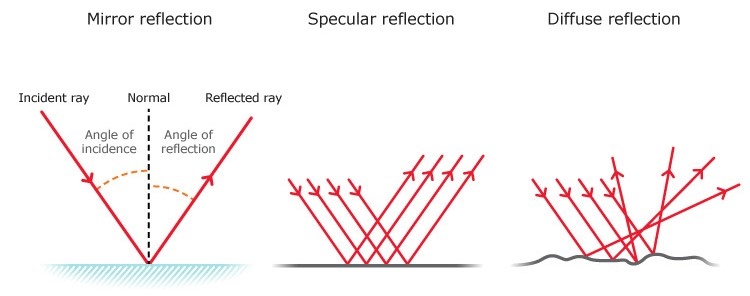
\includegraphics[width=5.5cm]{Physics/1st/Waves_and_optics/Images/diffuse.jpg}
  % \end{minipage}
  % Angle crític $\theta_c$: $$\theta_c:\theta_2=90^\circ$$
  % Dispersió cromàtica: L'índex de refracció depèn lleugerament de $\lambda$, $n(\lambda)$. Això explica fenòmens com l'arc de Sant Martí.
  % \begin{minipage}{\linewidth}
  %   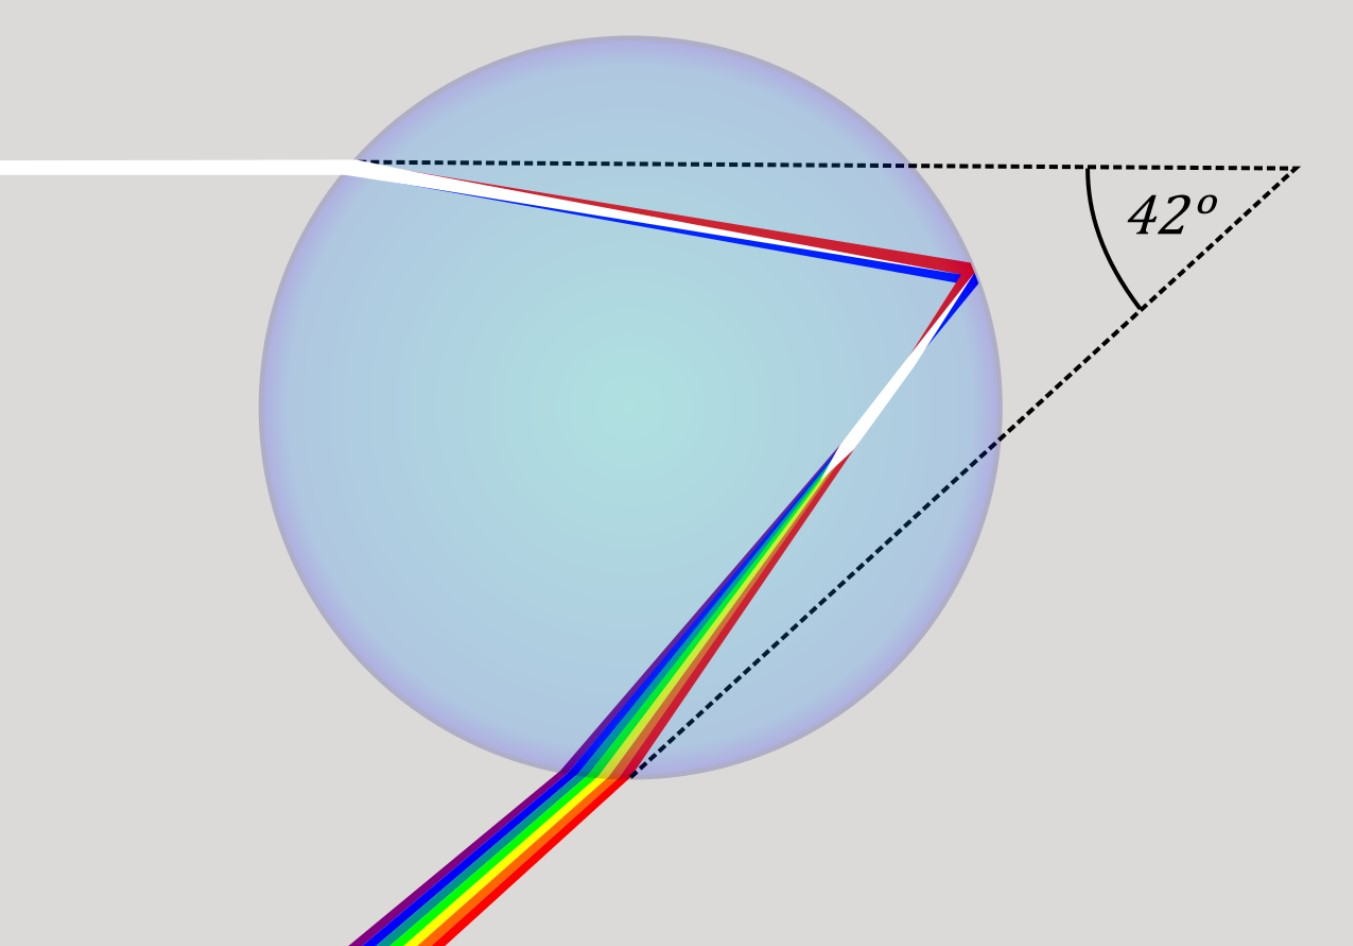
\includegraphics[width=5cm]{Physics/1st/Waves_and_optics/Images/rainbow.jpg}
  %   \captionof{figure}{Incidència i sortida d'un raig de llum en una gota d'aigua.}
  % \end{minipage}
  % Intensitat reflectida $I_r$ i transmesa $I_t$:
  % \begin{gather*}
  %   I_r=\left(\frac{n_1-n_2}{n_1+n_2}\right)^2I_0\\
  %   I_t=I_0-I_r
  % \end{gather*}
  % Làmina planoparal·lela:\newline
  % Angle d'entrada $\theta_1$ i de sortida $\theta_2'$: $$\theta_2'=\theta_1$$
  % Desplaçament $t$: $$t\approx d\theta_1\frac{n-1}{n}$$
  % {\footnotesize on s'ha emprat la notació de la \cref{plano}.}\newline
  % \begin{minipage}{\linewidth}
  %   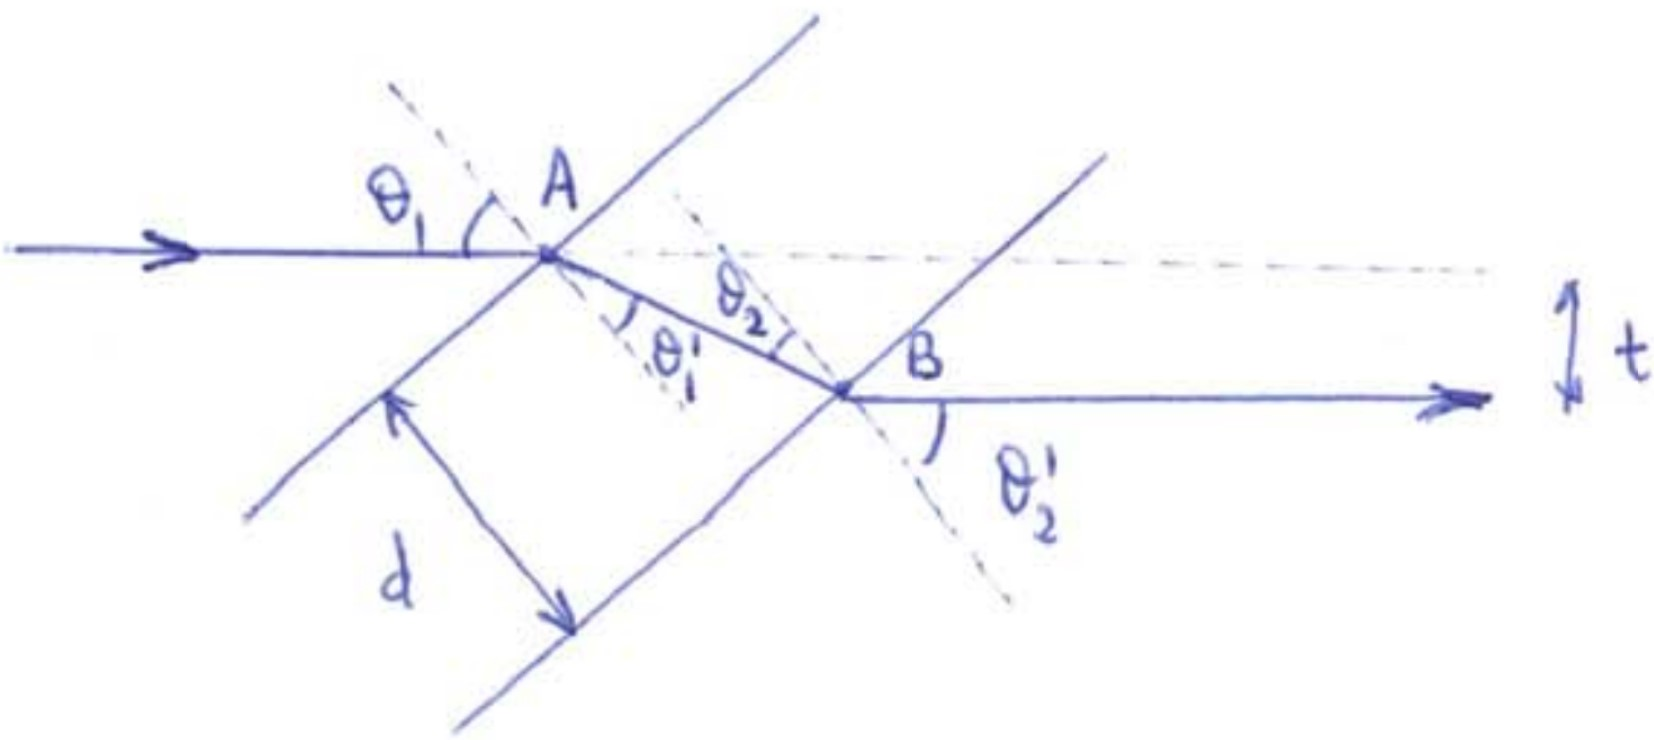
\includegraphics[width=5cm]{Physics/1st/Waves_and_optics/Images/plano.jpg}
  %   \captionof{figure}{}
  %   \label{plano}
  % \end{minipage}
  % Prisma òptic: \newline
  % En desviació mínima: $$\varepsilon_1'=\varepsilon_2=\frac{\alpha}{2}\qquad\varepsilon_1=\varepsilon_2'$$ {\footnotesize on s'ha emprat la notació de la \cref{pris}.}\newline
  % \begin{minipage}{\linewidth}
  %   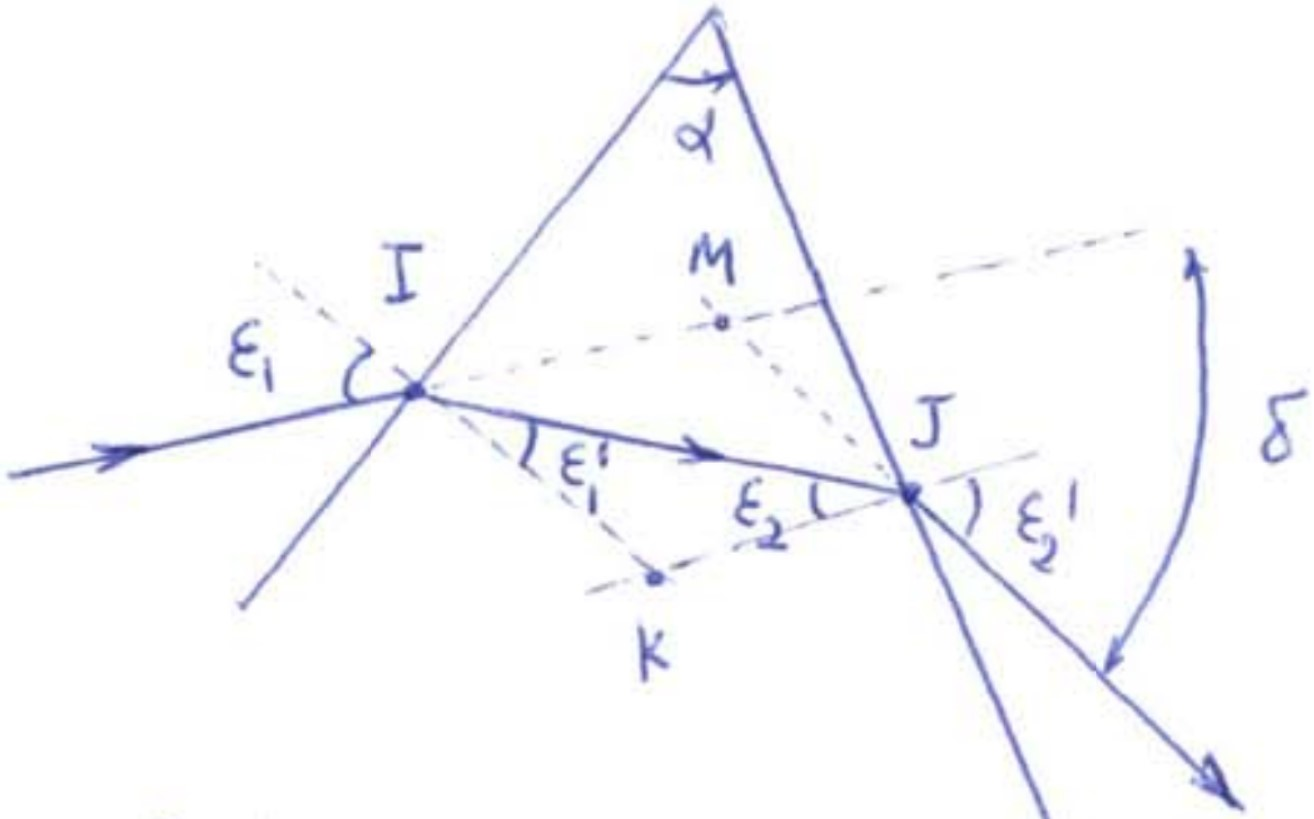
\includegraphics[width=5cm]{Physics/1st/Waves_and_optics/Images/prisma.jpg}
  %   \captionof{figure}{Prisma òptic. Aquí $\alpha$ és l'angle de refringència; $\varepsilon_1$, l'angle d'incidència, i $\delta(\varepsilon_1)$, l'angle de desviació. Aquest últim té un valor mínim.}
  %   \label{pris}
  % \end{minipage}
  % Polarització de la llum:
  % \begin{itemize}
  %   \item Polarització per absorció:\newline
  %         Camp elèctric final $E_1$:
  %         \begin{equation*}
  %           E_1=E_0\cos\theta
  %         \end{equation*}
  %         {\footnotesize on $E_0$ és el valor del camp elèctric inicial.}
  %         Intensitat final $I_1$:
  %         \begin{equation*}
  %           I_1=I_0\cos^2\theta
  %         \end{equation*}
  %         {\footnotesize on $I_0$ és la intensitat de la llum que arriba a l'analitzador.}\newline
  %         Grau de polarització lineal: $$G=\frac{I_{\text{max}}-I_{\text{min}}}{I_{\text{max}}+I_{\text{min}}}$$ {\footnotesize on $I_{\text{max}}$ i $I_{\text{min}}$ són les intensitats màxima i mínima, respectivament, transmeses mentre va girant l'analitzador.}\newline
  %         \begin{minipage}{\linewidth}
  %           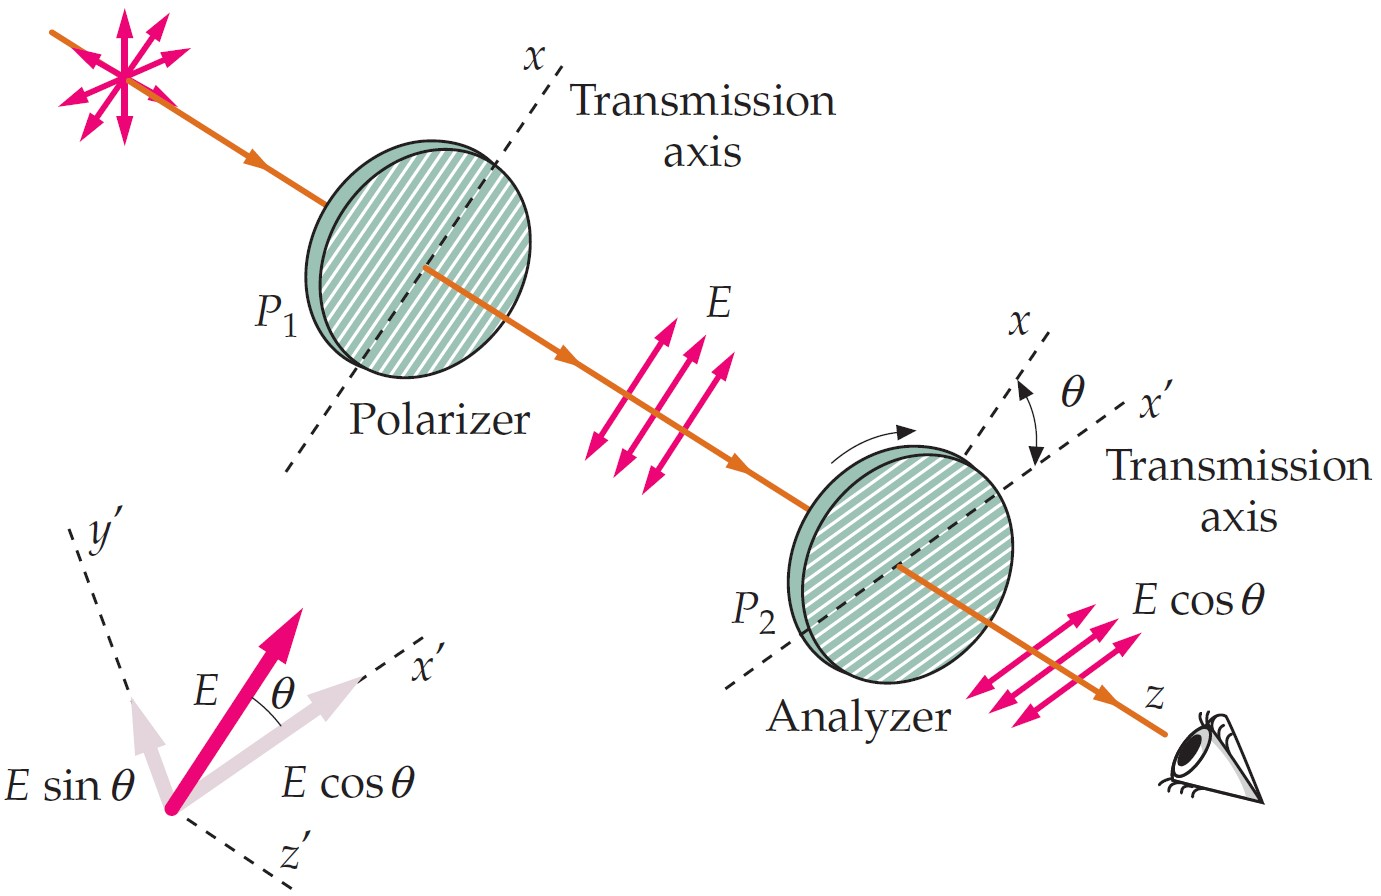
\includegraphics[width=5cm]{Physics/1st/Waves_and_optics/Images/pol1.jpg}
  %           \captionof{figure}{Polarització per absorció. El polaritzador deixa passar el camp elèctric en una sola direcció i l'analitzador rota aquesta direcció un angle $\theta$.}
  %         \end{minipage}
  %   \item Polarització per reflexió:
  %         $$\theta_2+\theta_B=\pi/2\implies\tan\theta_B=\frac{n_2}{n_1}$$ {\footnotesize on $\theta_B$ denota l'angle de Brewster.}\newline El feix reflectit és polaritzat linealment i el refractat és parcialment polaritzat linealment.
  %   \item Polarització per dispersió: Quan arriba la llum als àtoms, aquests vibraran de diferents maneres. Un àtom que vibri de manera vertical emetrà ones als costats horitzontals, és a dir, aquesta llum irradiada estarà polaritzada amb el camp elèctric paral·lel a l'eix $Y$. De forma anàloga s'expliquen els àtoms vibrant de manera horitzontal.
  %   \item Polarització per birrefringència o doble refracció: Com observem a la \cref{bir}, si tenim un feix incident amb dues components perpendiculars, una d'elles es retarda respecte de l'altra, ja que es propaguen a diferents velocitats. Si la làmina té un gruix $d$, això es traduirà en un canvi de fase $\Delta\varphi$. Aquest retard pot provocar un canvi en la polarització de la llum.
  %         $$\Delta\varphi=\frac{2\pi}{\lambda}d|n_e-n_o|$$ {\footnotesize on $n_e$ i $n_o$ són els índexs de refracció de cadascuna de les components del feix de llum i $\lambda$ és la longitud d'ona del feix de llum.}\newline
  %         \begin{minipage}{\linewidth}
  %           \centering
  %           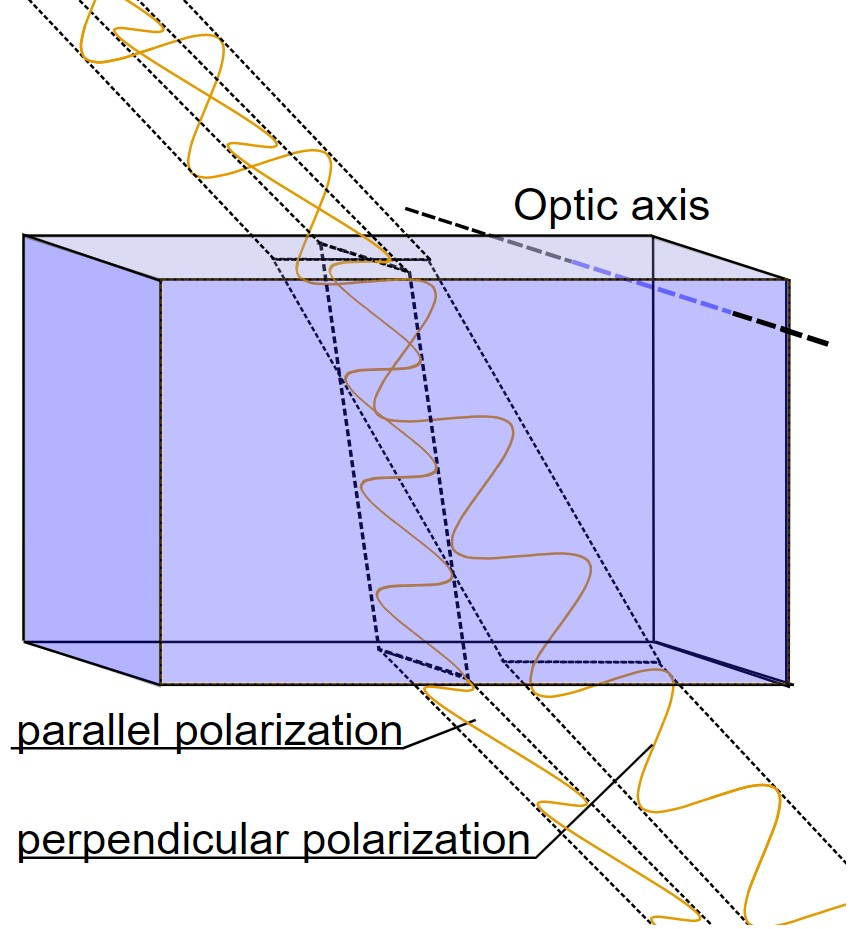
\includegraphics[width=4cm]{Physics/1st/Waves_and_optics/Images/dif.jpg}
  %           \captionof{figure}{Polarització per birrefringència.}
  %           \label{bir}
  %         \end{minipage}
  % \end{itemize}
  % \subsection{Òptica geomètrica}
  % Definicions:
  % \begin{itemize}
  %   \item Objecte: Lloc de l'espai d'on surt llum. Si és un punt $\rightarrow$ objecte puntual.
  %   \item Sistema òptic: Conjunt de superfícies que refracten i/o reflecteixen la llum.
  %   \item Eix òptic: En sistemes esfèrics, totes les superfícies comparteixen un eix de simetria de revolució. Aquest és l'eix òptic.
  %   \item Imatge puntual: Si després d'ex\-pe\-ri\-men\-tar alguna reflexió o refracció, els raigs o les seves prolongacions semblen provenir d'un punt o anar a un punt, allà es forma una imatge.
  %         \begin{itemize}
  %           \item Imatge real: Es produeix quan els raigs passen realment per la imatge.
  %           \item Imatge virtual: Es produeix quan són les prolongacions dels raigs les que passen per la imatge i, per tant, la llum no hi passa realment.
  %         \end{itemize}
  % \end{itemize}
  % Mirall pla:\newline
  % \begin{minipage}{\linewidth}
  %   \centering
  %   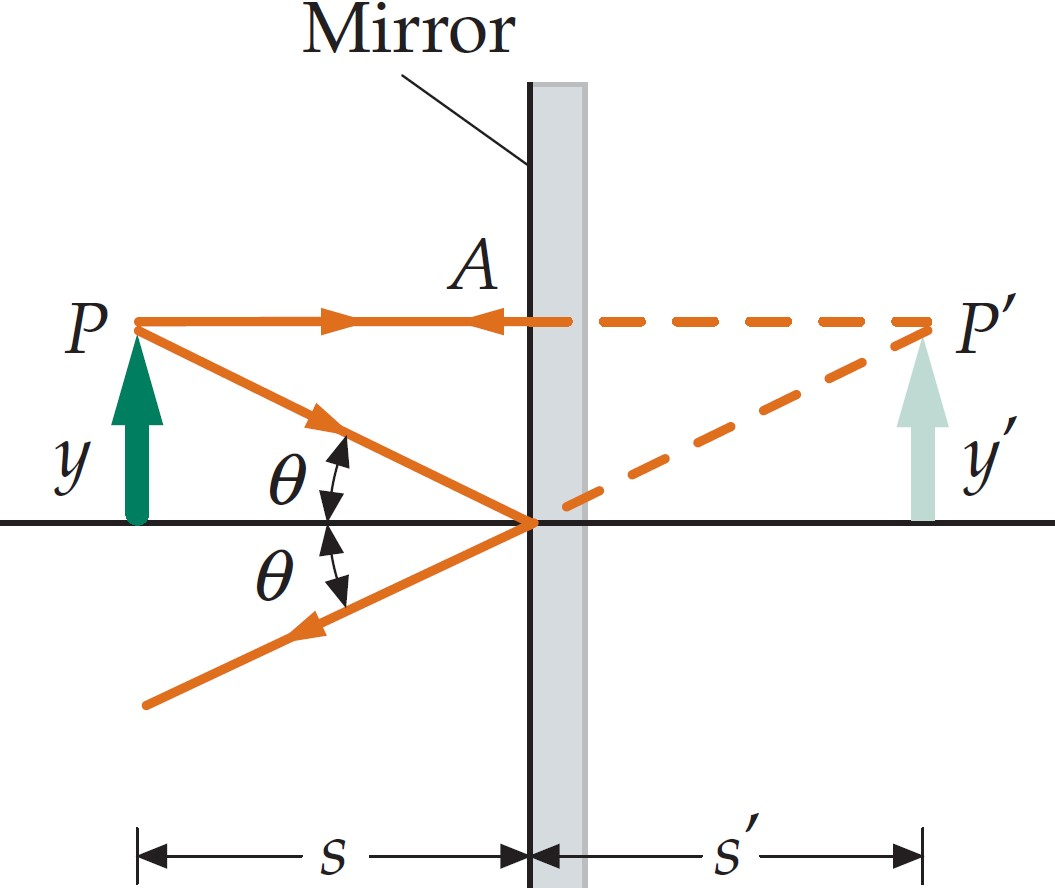
\includegraphics[width=4cm]{Physics/1st/Waves_and_optics/Images/pla.jpg}
  %   \captionof{figure}{Mirall pla. La imatge d'un punt objecte és un punt. La imatge és virtual. La imatge presenta inversió de polaritat (la imatge de la mà dreta és la mà esquerra).}
  % \end{minipage}
  % Aplicacions de combinacions de miralls plans: periscopi, retroreflector, calidoscopi.\newline
  % Criteri de signes (reflexió):
  % \begin{itemize}
  %   \item $s>0$ si l'objecte és a l'esquerra (davant) del mirall.
  %   \item $s'>0$ si la imatge és a l'esquerra (davant) del mirall.
  %   \item $r>0$ si el mirall és còncau, és a dir, si el centre de curvatura $C$ és a l'esquerra davant del mirall.
  %   \item $y>0$ si l'objecte està situat sobre l'eix òptic.
  %   \item $y'>0$ si la imatge està situada sobre l'eix òptic.
  %   \item $f>0$ si $F$ és a l'esquerra (davant) del mirall.
  %   \item $f'>0$ si $F'$ és a l'esquerra (davant) del mirall.
  % \end{itemize}
  % Definim la distància focal imatge del mirall com $f'$ de manera que si l'objecte està a l'infinit, $F'$ és el focus imatge del mirall. $$s\to\infty\implies s'\equiv f'=\frac{r}{2}$$ Definim la distància focal objecte $f$ com la distància a la qual s'ha de posar un objecte per tal que la seva imatge sigui a l'infinit. $$s'\to\infty\implies s\equiv f=\frac{r}{2}$$
  % Miralls esfèrics:\newline
  % Imatges per reflexió:\newline
  % \begin{minipage}{\linewidth}
  %   \centering
  %   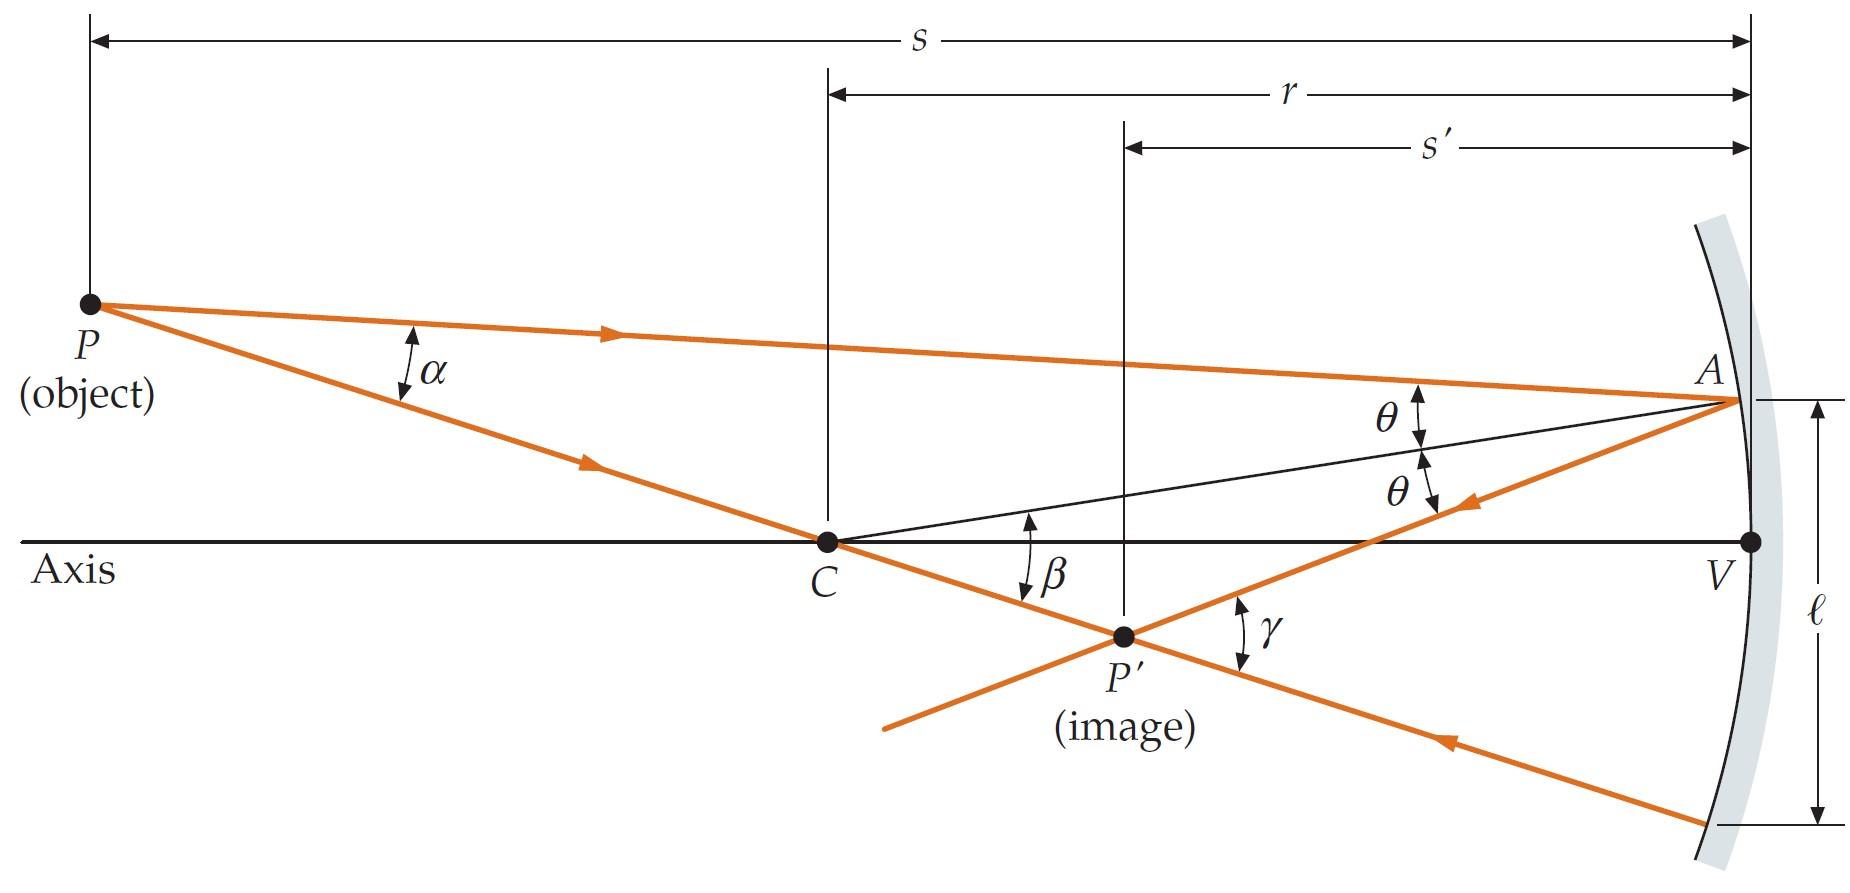
\includegraphics[width=\linewidth]{Physics/1st/Waves_and_optics/Images/conc.jpg}
  %   \captionof{figure}{Mirall esfèric còncau. $r$ és el radi de curvatura. En aquest cas la imatge és real.}
  % \end{minipage}
  % Equació del mirall:
  % $$\frac{1}{s}+\frac{1}{s'}=\frac{1}{f'}$$ {\footnotesize on $f'=r/2$ és la distància focal.}\newline
  % Augment lateral $\beta'$:
  % $$\beta'=\frac{y'}{y}=-\frac{s'}{s}$$
  % Diagrama de raigs per miralls:\newline
  % \begin{minipage}{\linewidth}
  %   \centering
  %   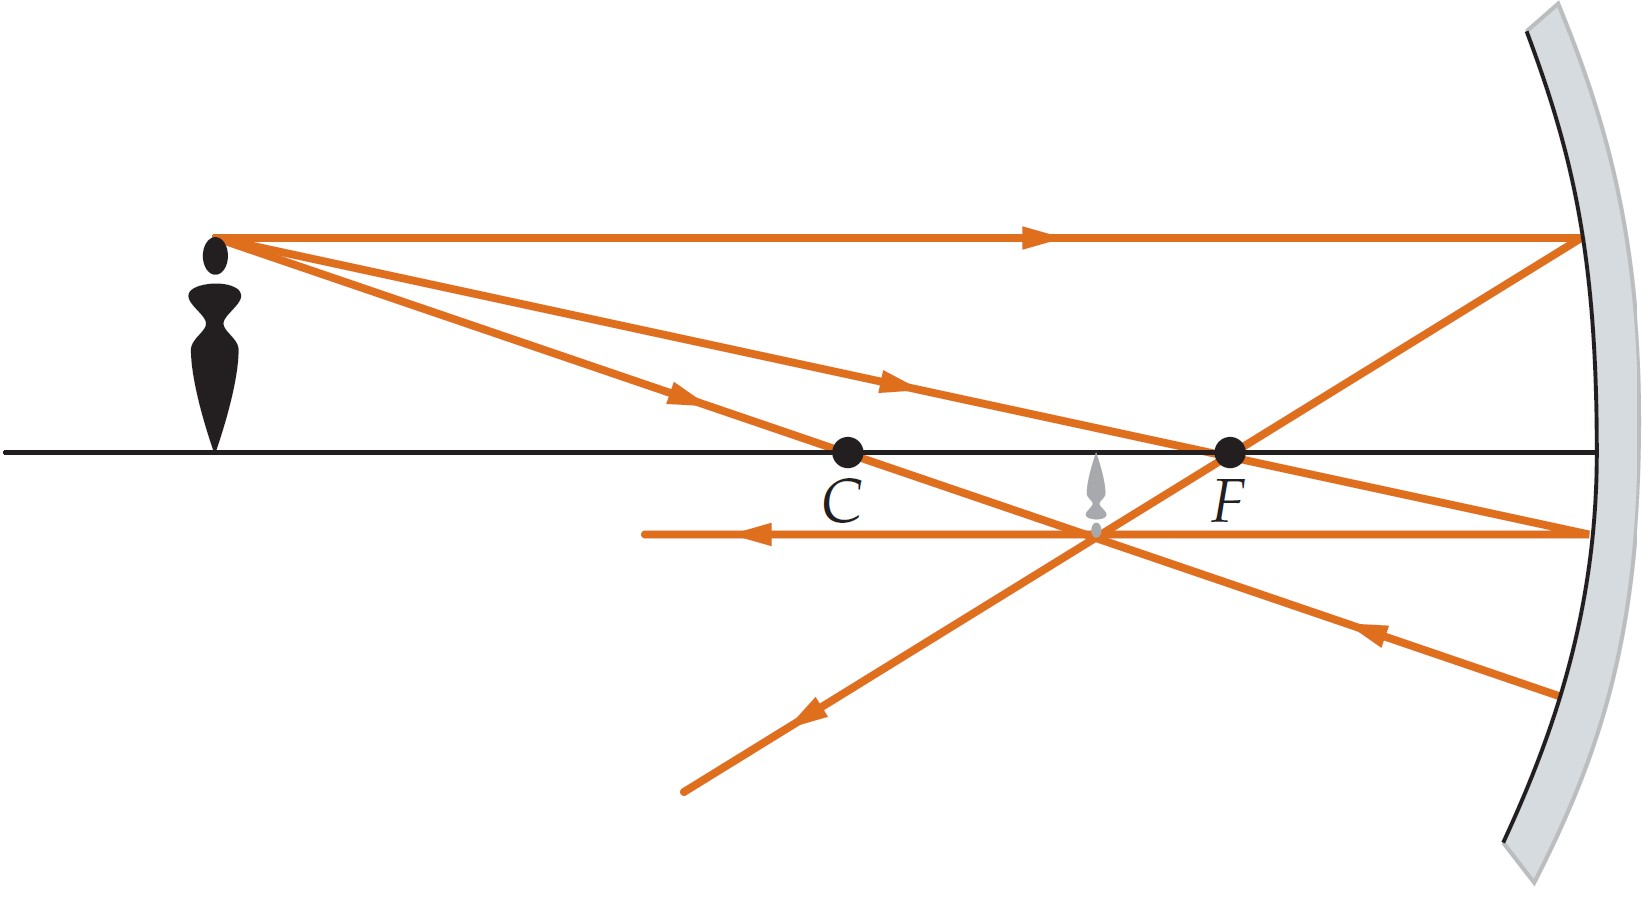
\includegraphics[width=4cm]{Physics/1st/Waves_and_optics/Images/raigs.jpg}
  %   \captionof{figure}{Diagrama de raigs. De dalt a baix: el primer raig és paral·lel a l'eix òptic i quan es reflecteix passa per $F$; el segon passa per $F$ i es reflecteix paral·lelament a l'eix òptic, i el tercer incideix passant per $C$ (centre de curvatura) i es reflecteix sobre si mateix.}
  % \end{minipage}
  % Criteri de signes (refracció):
  % \begin{itemize}
  %   \item $s>0$ si l'objecte és a l'esquerra (davant) del mirall.
  %   \item $s'>0$ si la imatge és a la dreta (darrere) del mirall.
  %   \item $r>0$ si el centre de curvatura $C$ és a la dreta (darrere) del mirall.
  % \end{itemize}
  % \begin{minipage}{\linewidth}
  %   \centering
  %   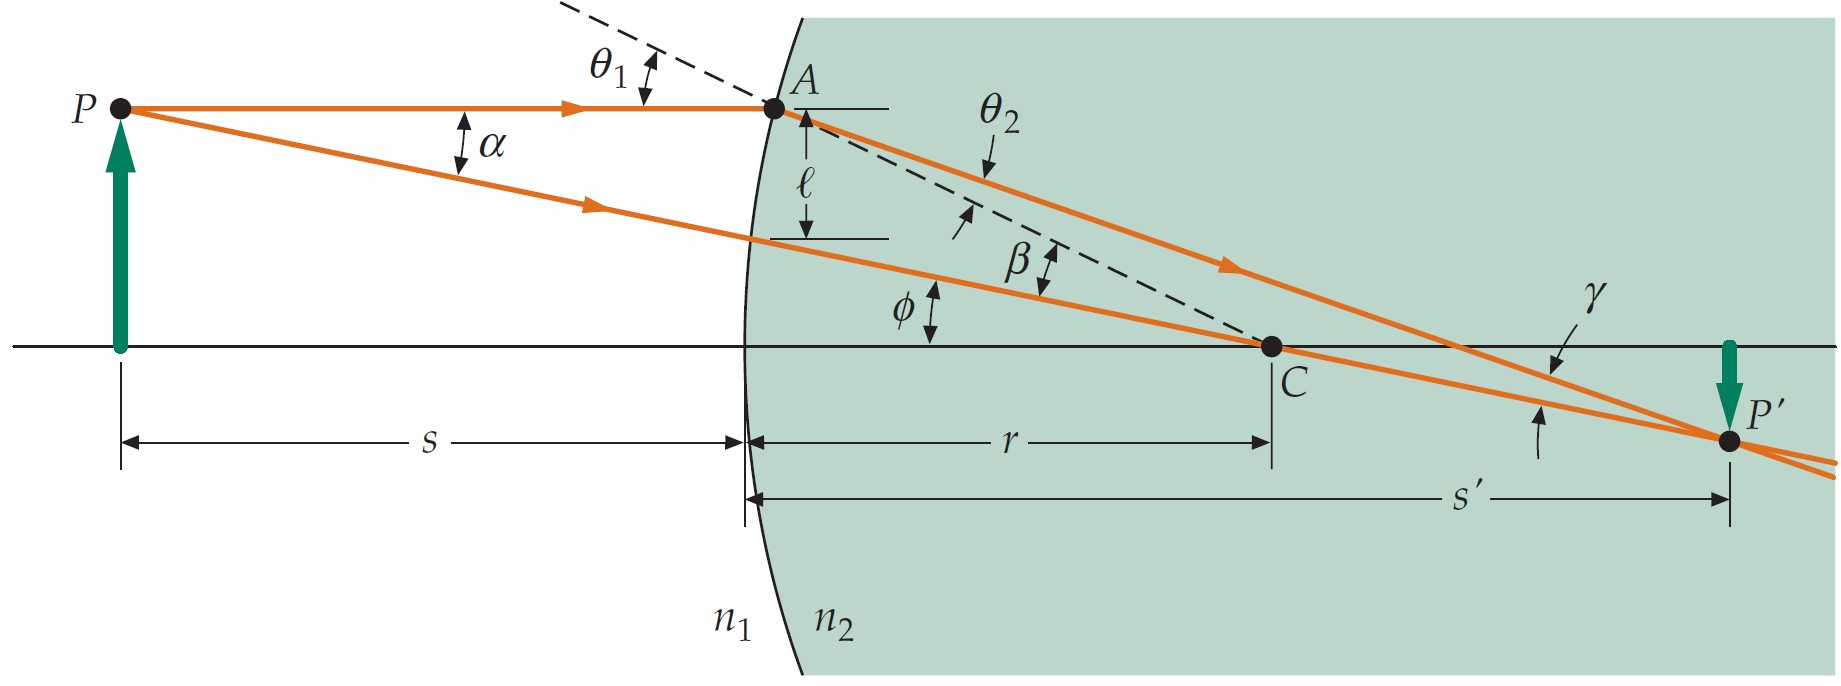
\includegraphics[width=\linewidth]{Physics/1st/Waves_and_optics/Images/ref.jpg}
  %   \captionof{figure}{Imatge formada per refracció.}
  % \end{minipage}
  % Equació per a la refracció:
  % $$\frac{n_1}{s}+\frac{n_2}{s'}=\frac{n_2-n_1}{r}$$
  % Augment lateral $\beta'$:
  % $$\beta'=\frac{y'}{y}=-\frac{n_1s'}{n_2s}$$
  % Lents primes:\newline Considerem lents d'un material amb índex de refracció $n$ envoltades d'aire ($n_{\text{aire}}=1$)
  % \begin{minipage}{\linewidth}
  %   \centering
  %   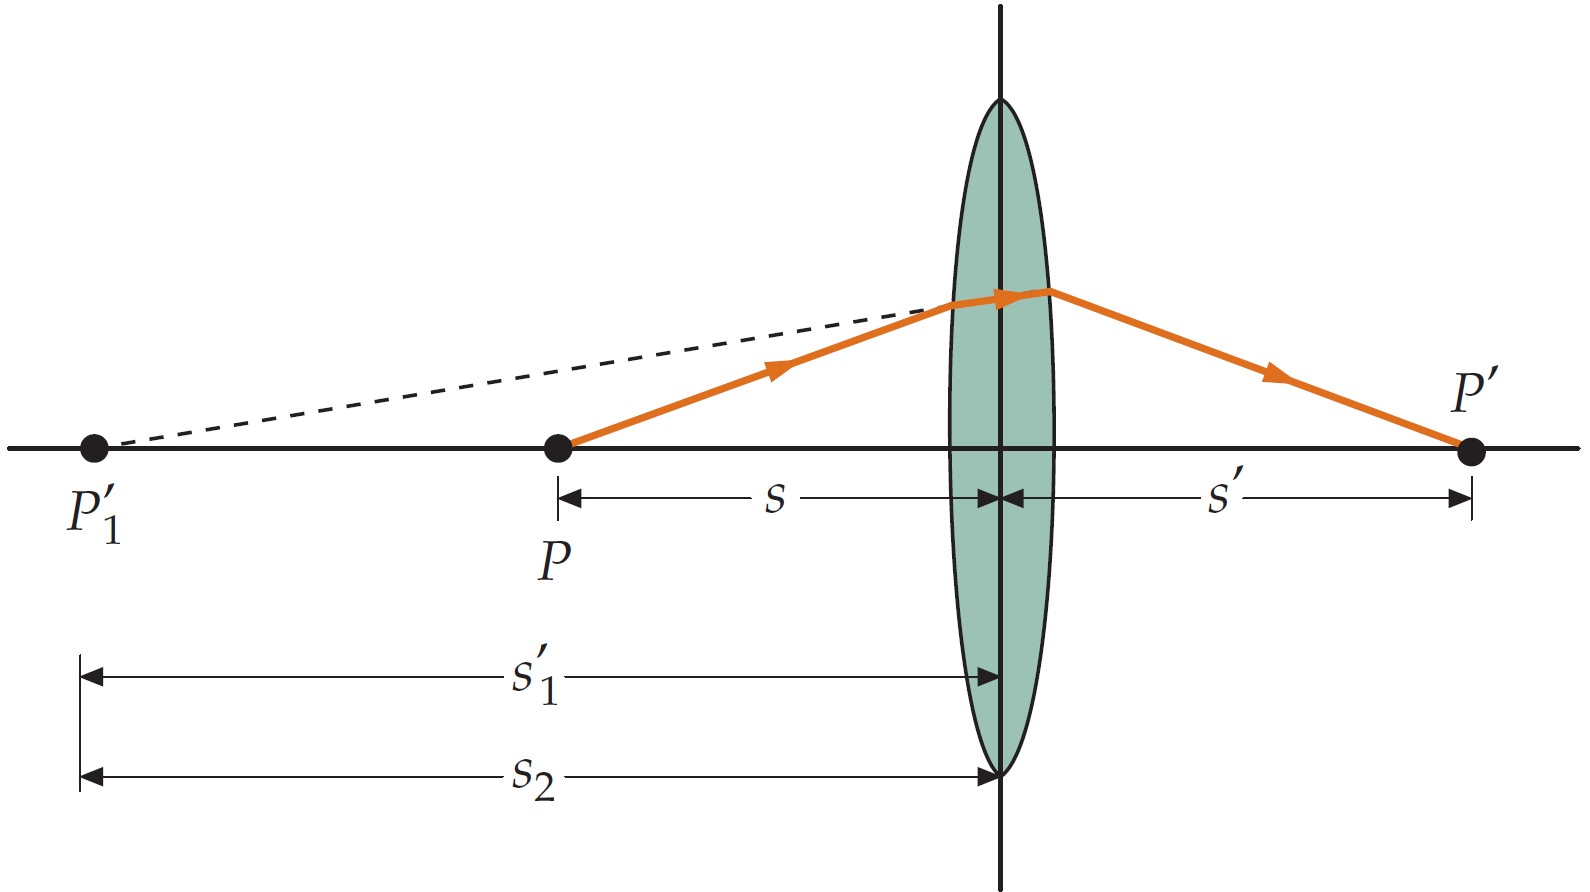
\includegraphics[width=4cm]{Physics/1st/Waves_and_optics/Images/lens.jpg}
  %   \captionof{figure}{Lent prima convergent de radis $r_1$ (arc de circumferència de l'esquerra) i $r_2$ (arc de circumferència de la dreta).}
  %   \label{conv}
  % \end{minipage}
  % Equació per a la lent prima: $$\frac{1}{s}+\frac{1}{s'}=(n-1)\left(\frac{1}{r_1}-\frac{1}{r_2}\right)=\frac{
  %     1}{f'}$$ {\footnotesize on hem definit la distància focal imatge de la lent com $\frac{
  %         1}{f'}=(n-1)\left(\frac{1}{r_1}-\frac{1}{r_2}\right)$}\newline
  % Tipus de lents:
  % \begin{itemize}
  %   \item Convergents: {\footnotesize vegeu la \cref{conv}.}
  %   \item Divergents:\newline
  %         \begin{minipage}{\linewidth}
  %           \centering
  %           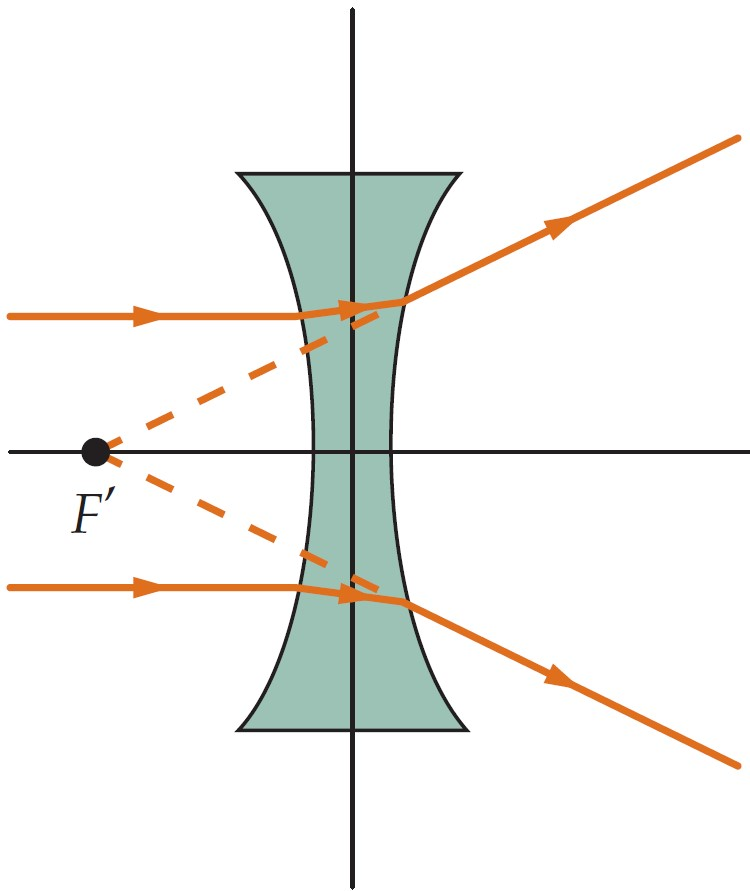
\includegraphics[width=2cm]{Physics/1st/Waves_and_optics/Images/div.jpg}
  %           \captionof{figure}{Lent prima divergent.}
  %         \end{minipage}
  % \end{itemize}
  % Potència d'una lent: $$P=\frac{1}{f'}$$ {\footnotesize on $[f']=m$ i $[P]=D$ (Diòptries)}\newline
  % Marxa dels raigs a través de lents primes:
  % \begin{minipage}{\linewidth}
  %   \centering
  %   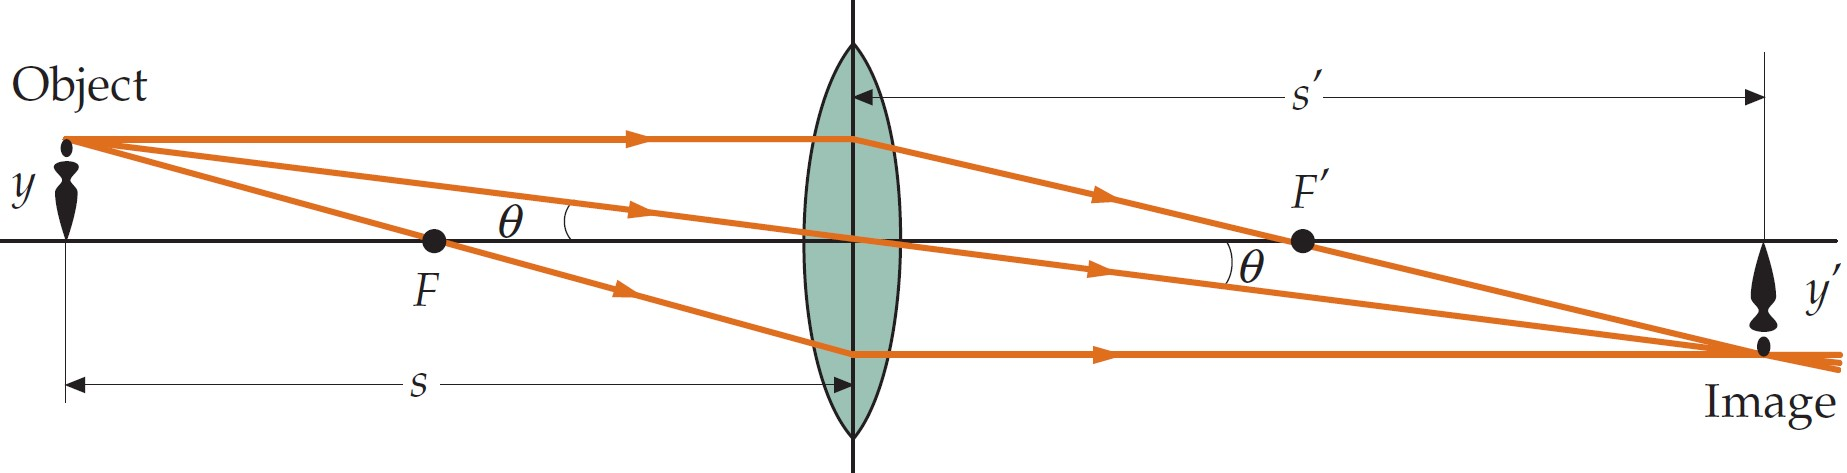
\includegraphics[width=\linewidth]{Physics/1st/Waves_and_optics/Images/raiglen.jpg}
  %   \captionof{figure}{Lent prima convergent.}
  % \end{minipage}
  % \begin{minipage}{\linewidth}
  %   \centering
  %   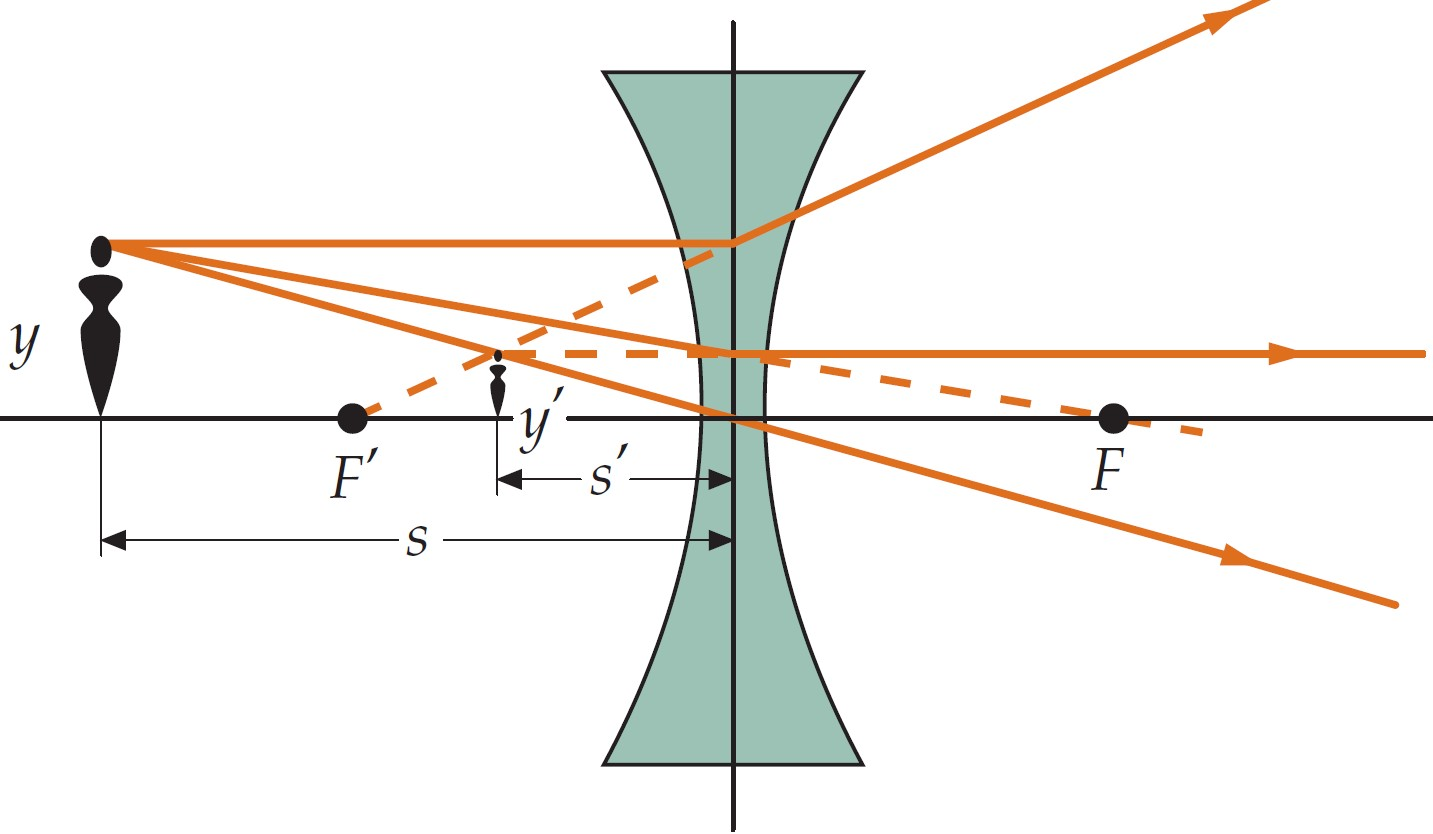
\includegraphics[width=4cm]{Physics/1st/Waves_and_optics/Images/raiglen2.jpg}
  %   \captionof{figure}{Lent prima divergent.}
  % \end{minipage}
  % Combinacions de lents primes: La imatge de l'objecte a través de la primera lent és l'objecte de la segona lent. $$s_2=d-s_1'$$ {\footnotesize on $d$ és la distància de separació entre les dues lents.}
  % Dues lents primes en contacte són equivalents a una única lent prima de focal $f_T'$ de manera que: $$\frac{1}{f_T'}=\frac{1}{f_1'}+\frac{1}{f_2'}\qquad P_T=P_1+P_2$$ {\footnotesize on $P_i$ és la potència de la lent $i$-èssima.}
  % $$\frac{1}{s_1}+\frac{1}{s_2'}=\frac{1}{f_T'}$$
  % Aberracions: Comportament ``no perfecte" d'una lent o d'un sistema òptic. La imatge d'un objecte puntual no és un punt imatge.
  % Tipus d'aberracions:
  % \begin{itemize}
  %   \item Aberració esfèrica:\newline
  %         \begin{minipage}{\linewidth}
  %           \centering 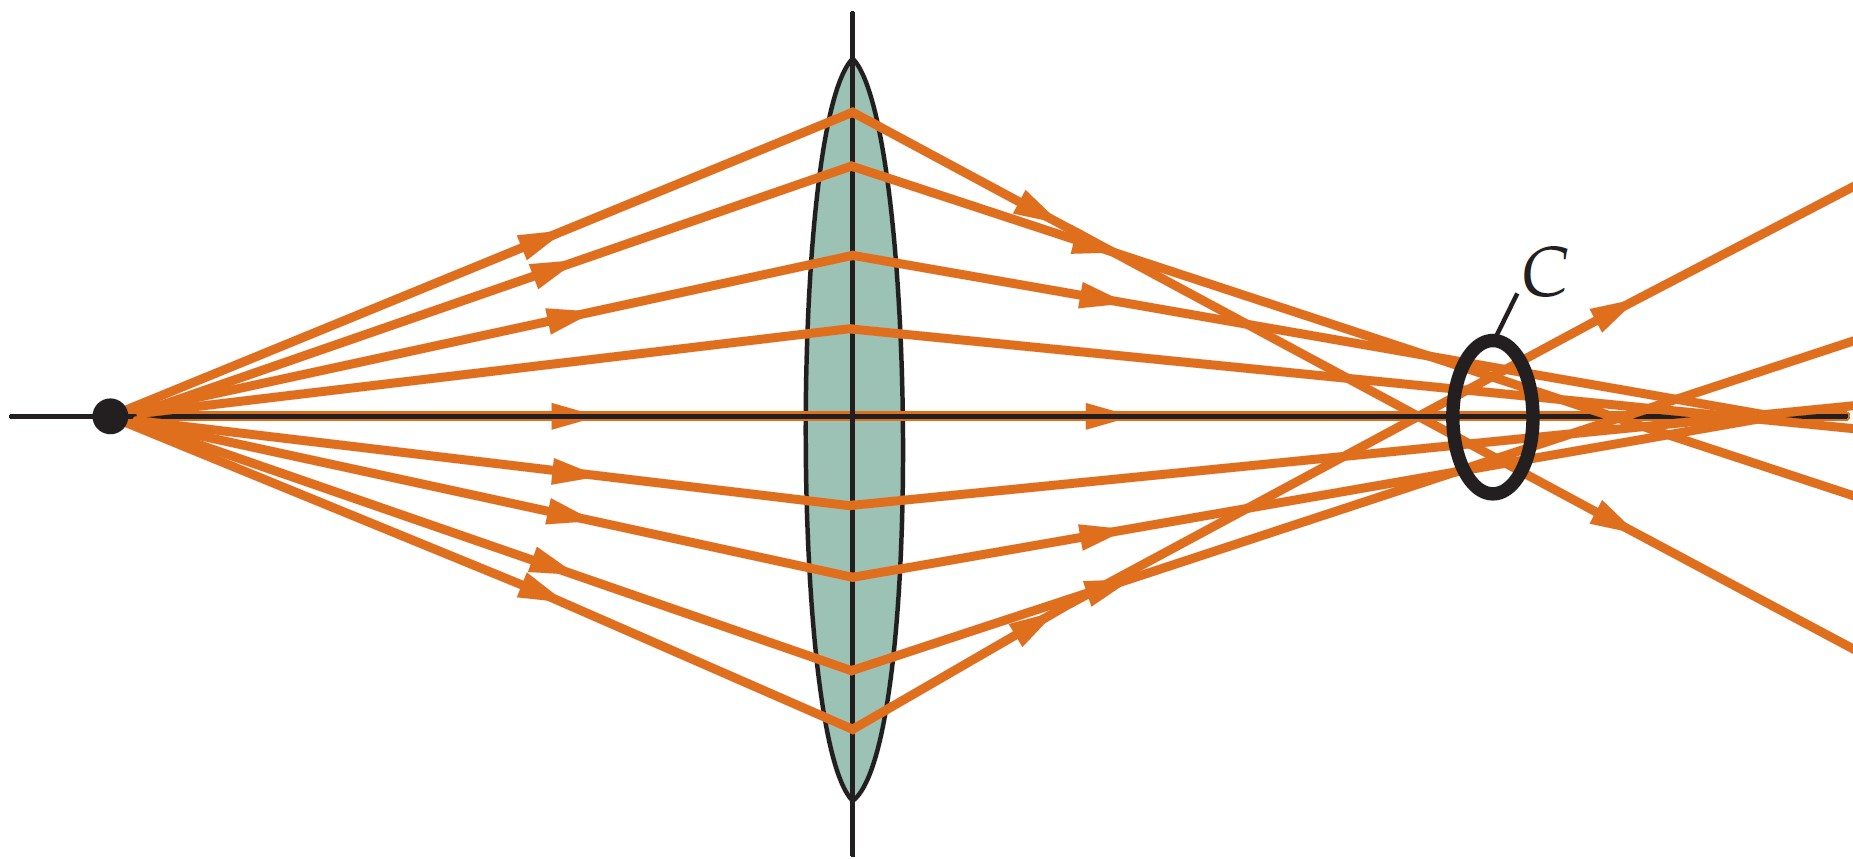
\includegraphics[width=4cm]{Physics/1st/Waves_and_optics/Images/aberr1.jpg}
  %           \captionof{figure}{Aberració esfèrica.}
  %         \end{minipage}
  %         \begin{minipage}{\linewidth}
  %           \centering 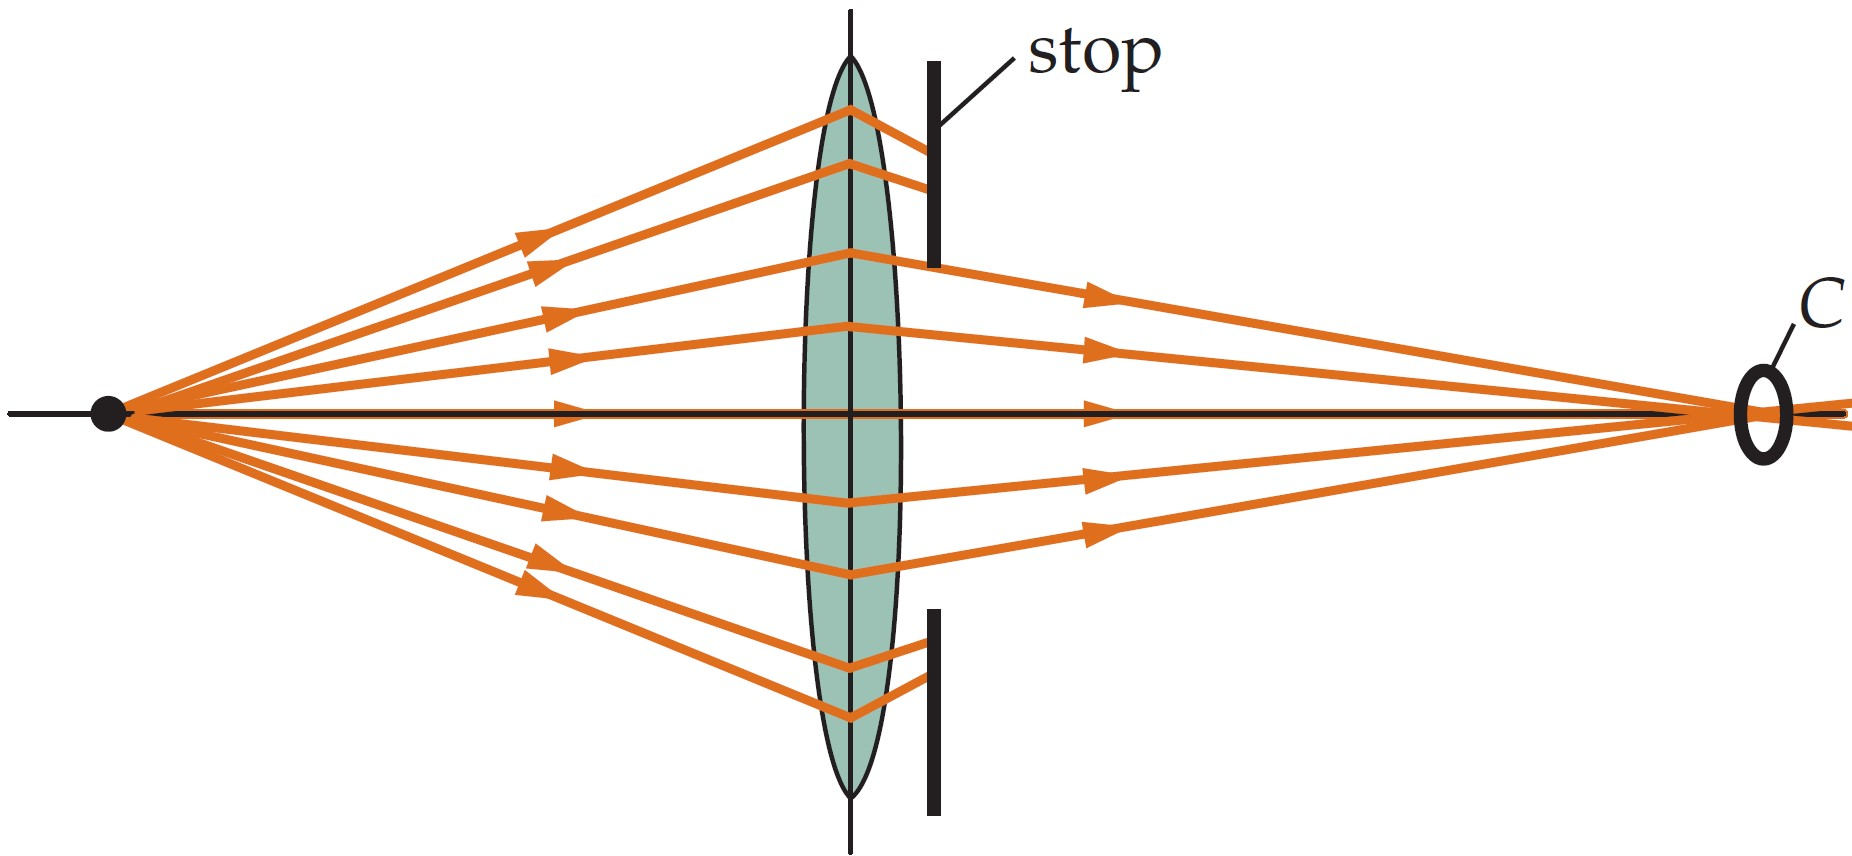
\includegraphics[width=4cm]{Physics/1st/Waves_and_optics/Images/aberr2.jpg}
  %           \captionof{figure}{Aberració esfèrica corregida amb un diafragma que redueix el nombre de raigs aconseguint que la imatge sigui puntual.}
  %         \end{minipage}
  % \end{itemize}
  % Si l'objecte és fora de l'eix, tenim altres aberracions com coma o astigmatisme.\newline
  % Si l'objecte és extens, podem tenir també curvatura de camp o distorsió.\newline
  % Si, a més, la llum incident és blanca (composta de diferents $\lambda$'s), tenim aberració cromàtica.\newline
  % Pels miralls també tenim totes aquestes aberracions excepte la cro\-mà\-ti\-ca.\newline
  % Altres defectes visuals:
  % \begin{itemize}
  %   \item Hipermetropia:\newline
  %         \begin{minipage}{\linewidth}
  %           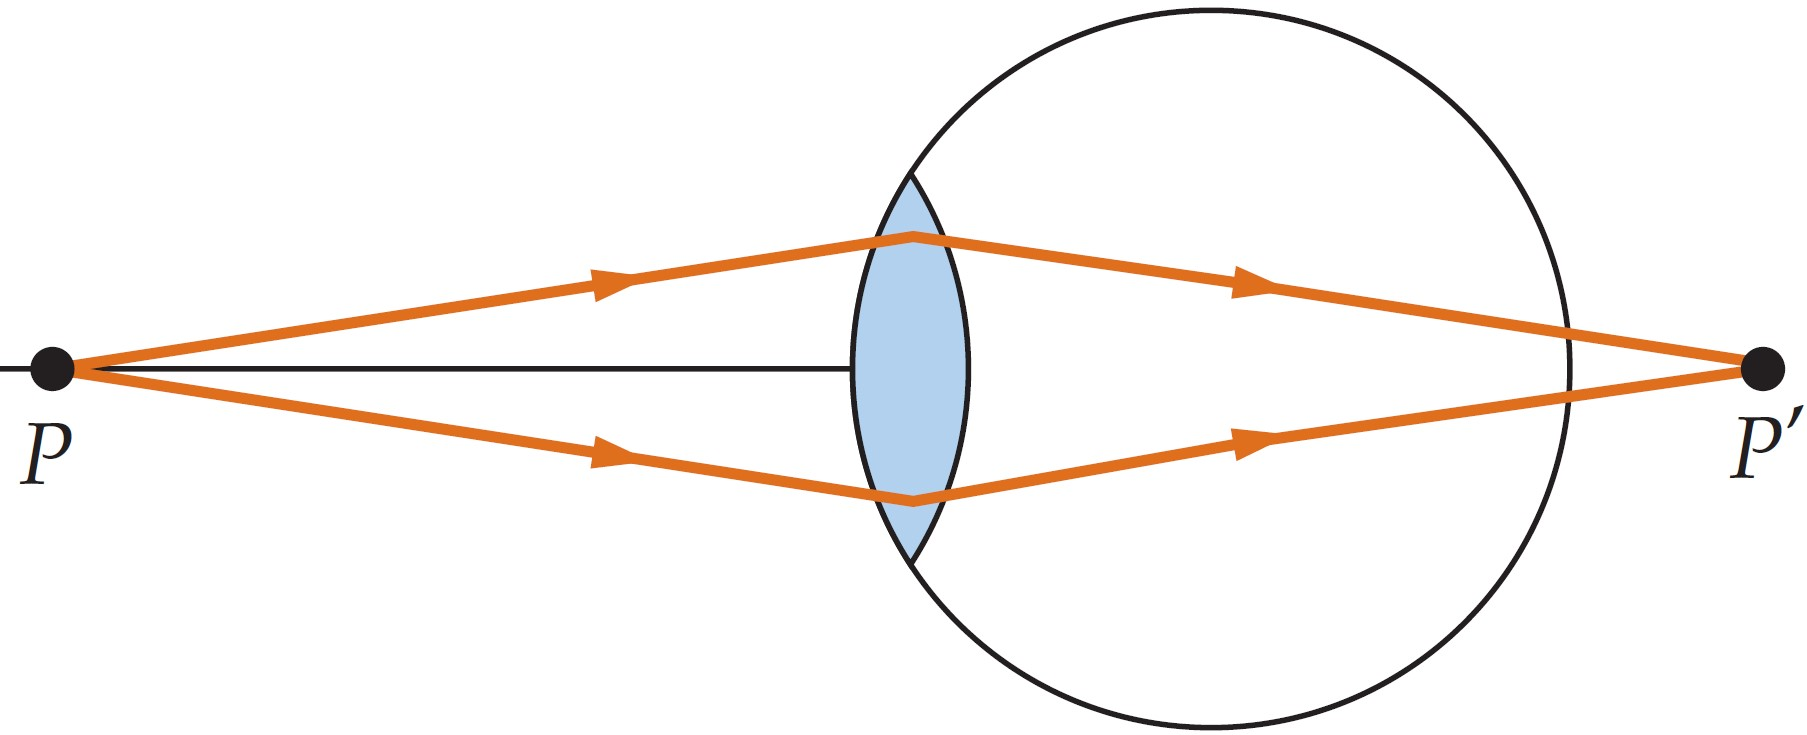
\includegraphics[width=\linewidth]{Physics/1st/Waves_and_optics/Images/hip.jpg}
  %           \captionof{figure}{Hipermetropia.}
  %         \end{minipage}\hspace{0.15cm}
  %         \begin{minipage}{\linewidth}
  %           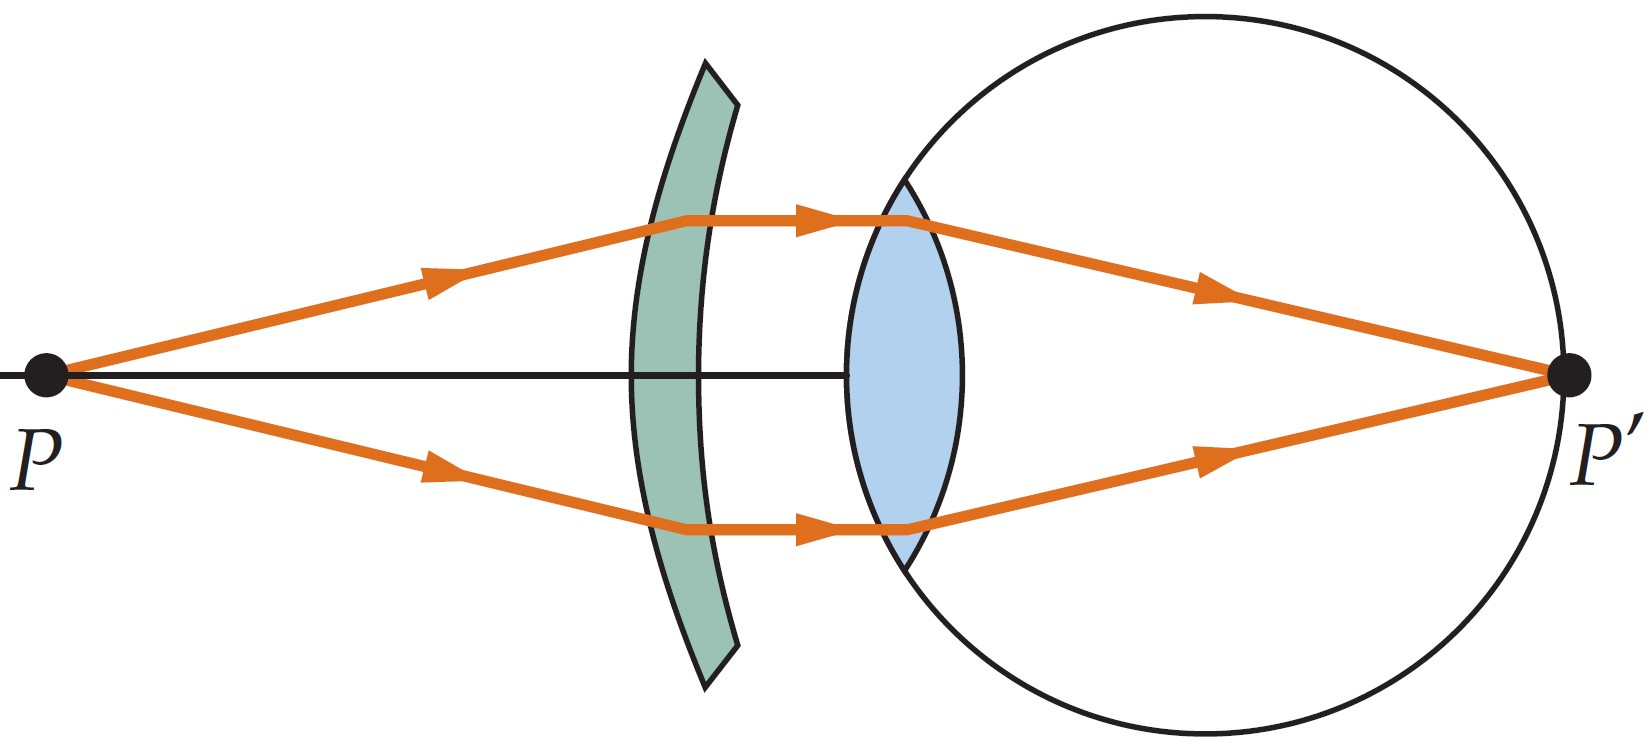
\includegraphics[width=\linewidth]{Physics/1st/Waves_and_optics/Images/hip1.jpg}
  %           \captionof{figure}{Hipermetropia corregida amb una lent convergent.}
  %         \end{minipage}
  %   \item Miopia:\newline
  %         \begin{minipage}{\linewidth}
  %           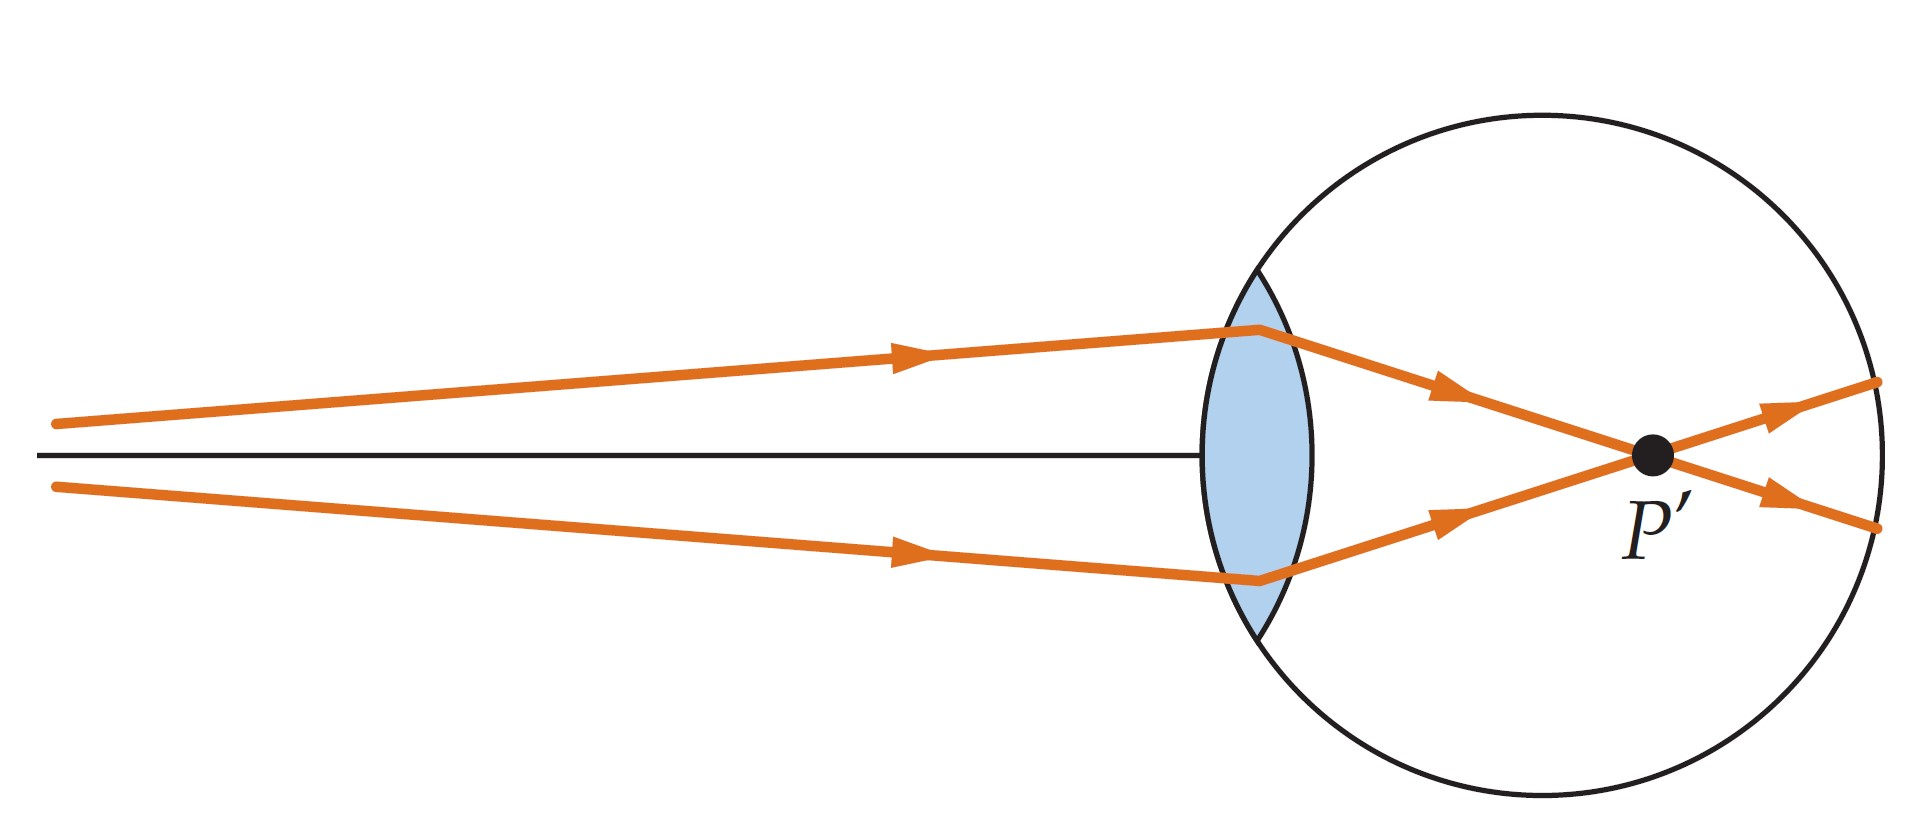
\includegraphics[width=\linewidth]{Physics/1st/Waves_and_optics/Images/mio.jpg}
  %           \captionof{figure}{Miopia.}
  %         \end{minipage}\hspace{0.15cm}
  %         \begin{minipage}{\linewidth}
  %           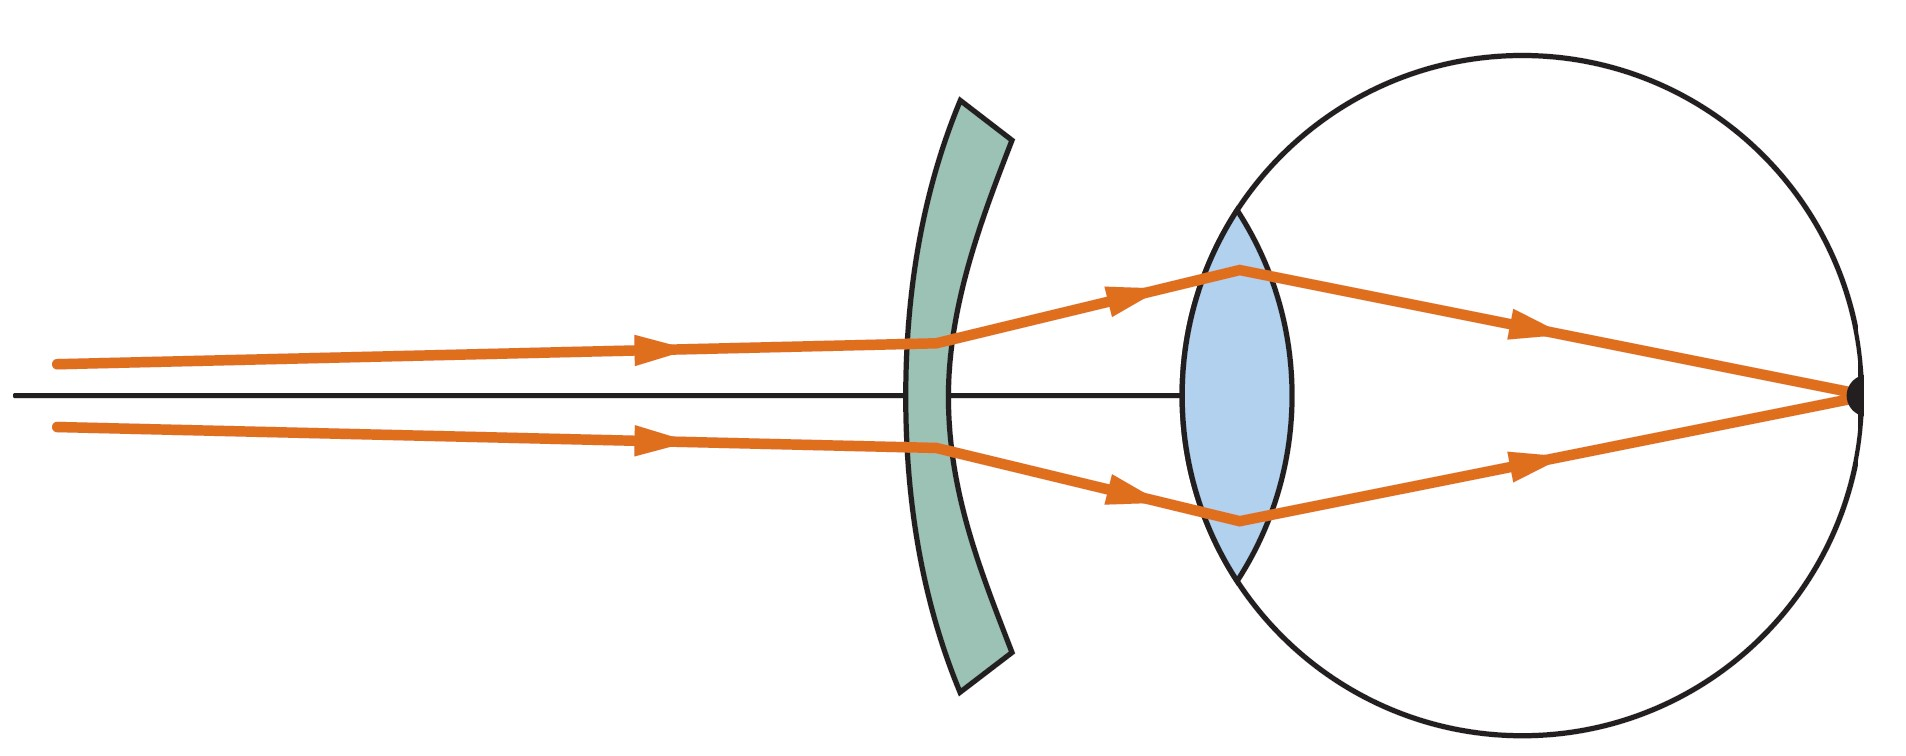
\includegraphics[width=\linewidth]{Physics/1st/Waves_and_optics/Images/mio1.jpg}
  %           \captionof{figure}{Miopia cor\-re\-gi\-da amb una lent divergent.}
  %         \end{minipage}
  %   \item Astigmatisme: Falta de simetria es\-fè\-ri\-ca de la còrnia o del cristal·lí, que té una curvatura diferent en un pla que en un altre. Es corregeix amb una lent cil·líndrica que compensa la manca de simetria esfèrica.
  %   \item Presbícia o vista cansada: Gràcies a la deformació del cristal·lí podem enfocar l'ull des de l'infinit fins al punt pròxim ($\sim7$ cm per als nadons; $\sim25$ cm per als adults, i $\sim100$ cm per a la tercera edat). Amb l'edat, la pèrdua de fle\-xi\-bi\-li\-tat del cristal·lí allunya la posició del punt pròxim.
  %   \item Daltonisme: Percepció incorrecta dels co\-lors per una diferent proporció de conus (fotoreceptors) vermells $-$ verds $-$ blaus.
  % \end{itemize}
  % Mida aparent d'un objecte:\newline
  % \begin{minipage}{\linewidth}
  %   \centering
  %   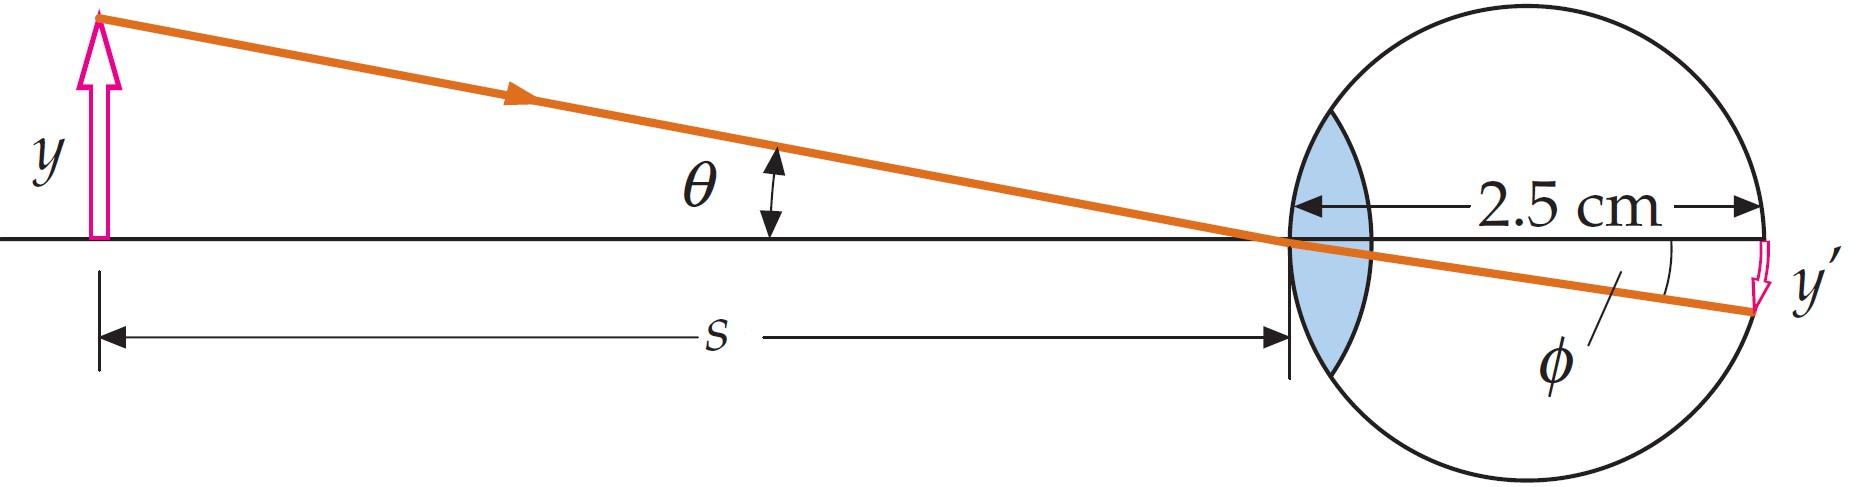
\includegraphics[width=\linewidth]{Physics/1st/Waves_and_optics/Images/mida.jpg}
  %   \captionof{figure}{}
  % \end{minipage} $$y'\approx2,5\text{ cm}\frac{y}{n_{\text{ull}}s}$$ {\footnotesize on $n_{\text{ull}}\sim1,336-1,406$ variant lleugerament segons a quina part de l'ull ens referim.}\newline
  % Lupa (o lent d'augment):\newline
  % \begin{minipage}{\linewidth}
  %   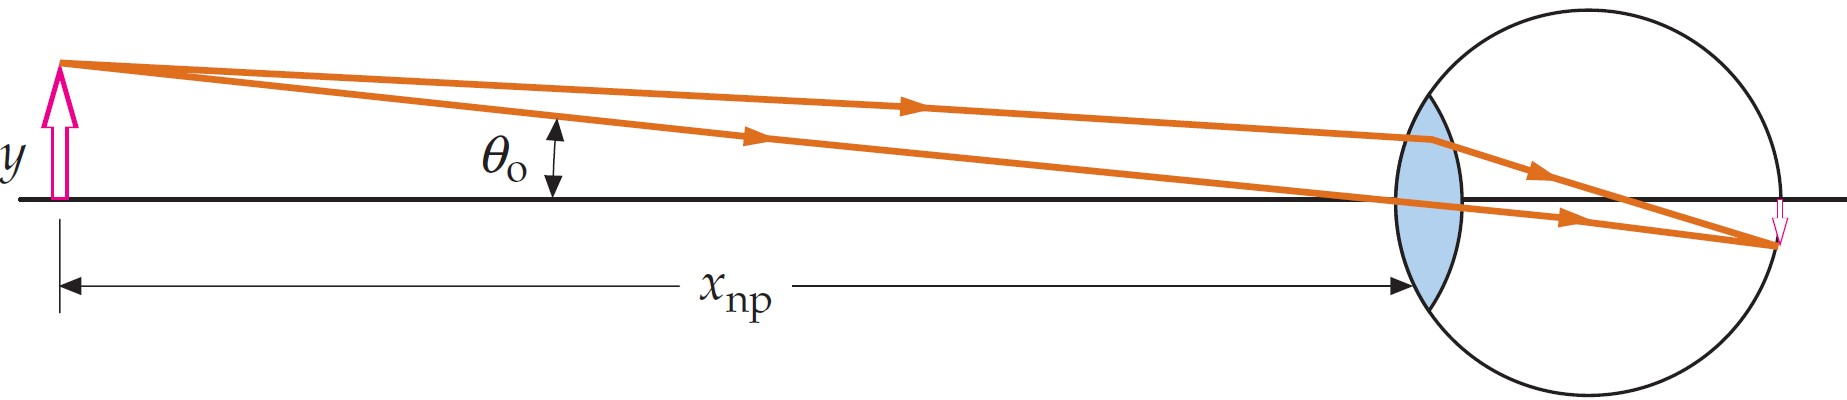
\includegraphics[width=\linewidth]{Physics/1st/Waves_and_optics/Images/senselup.jpg}
  %   \captionof{figure}{Observació d'un objecte d'alçada $y$ a una distància $x_{\text{np}}=25$ cm de l'ull. La mida aparent és $\theta_0=y/x_{\text{np}}=y/(25\text{ cm})$.}
  % \end{minipage}
  % \begin{minipage}{\linewidth}
  %   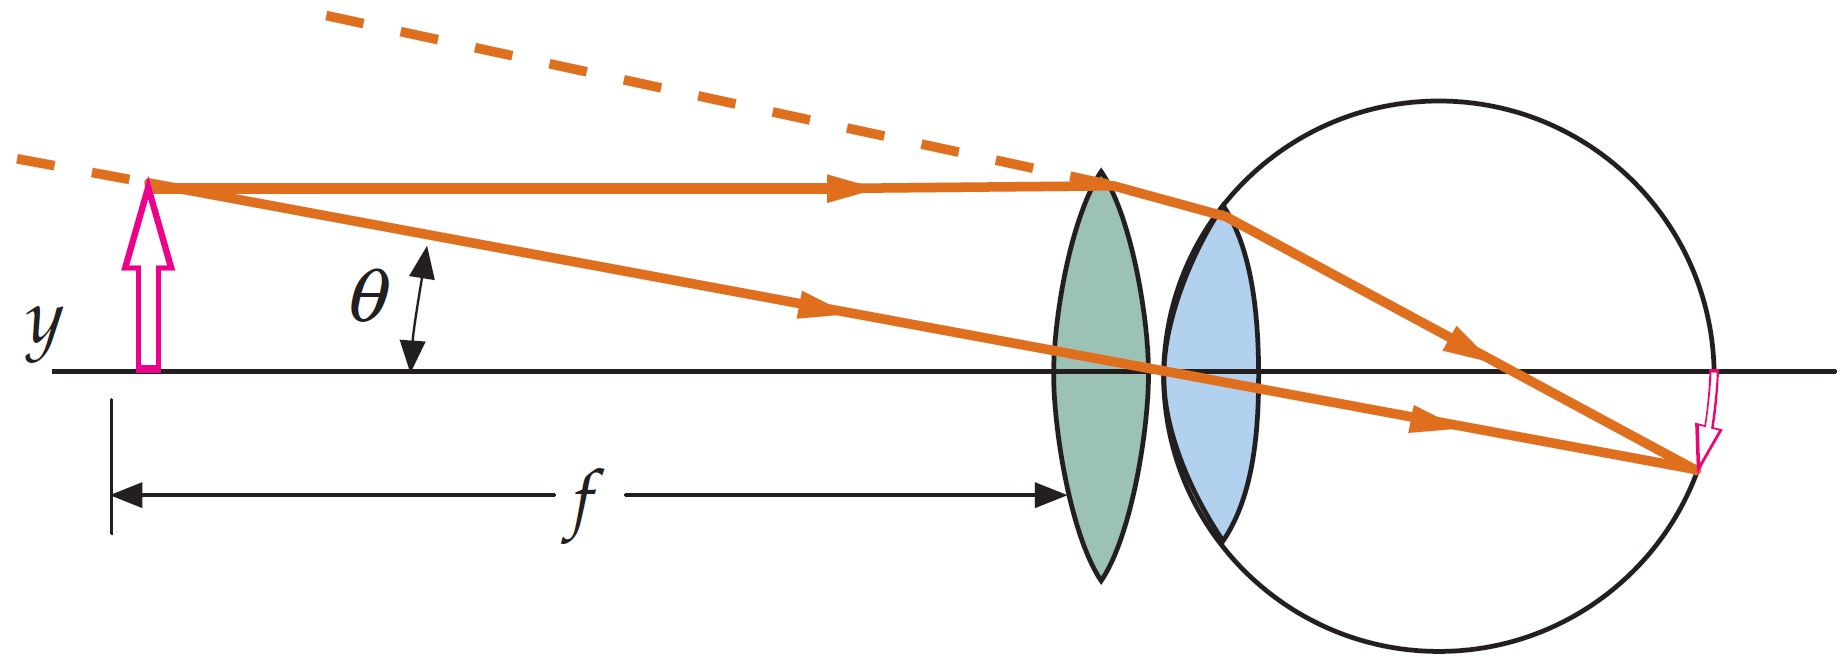
\includegraphics[width=\linewidth]{Physics/1st/Waves_and_optics/Images/lup.jpg}
  %   \captionof{figure}{Observació d'un objecte d'alçada $y$ a una distància $f<x_{\text{np}}$ de l'ull (i que, per tant, l'ull no podria veure nítida) amb la implementació d'una lupa. La mida aparent és $\theta=y/f$.}
  % \end{minipage}
  % Amplificació angular: $$\frac{\theta}{\theta_0}=\frac{25\text{ cm}}{f}$$
  % Microscopi compost:\newline
  % \begin{minipage}{\linewidth}
  %   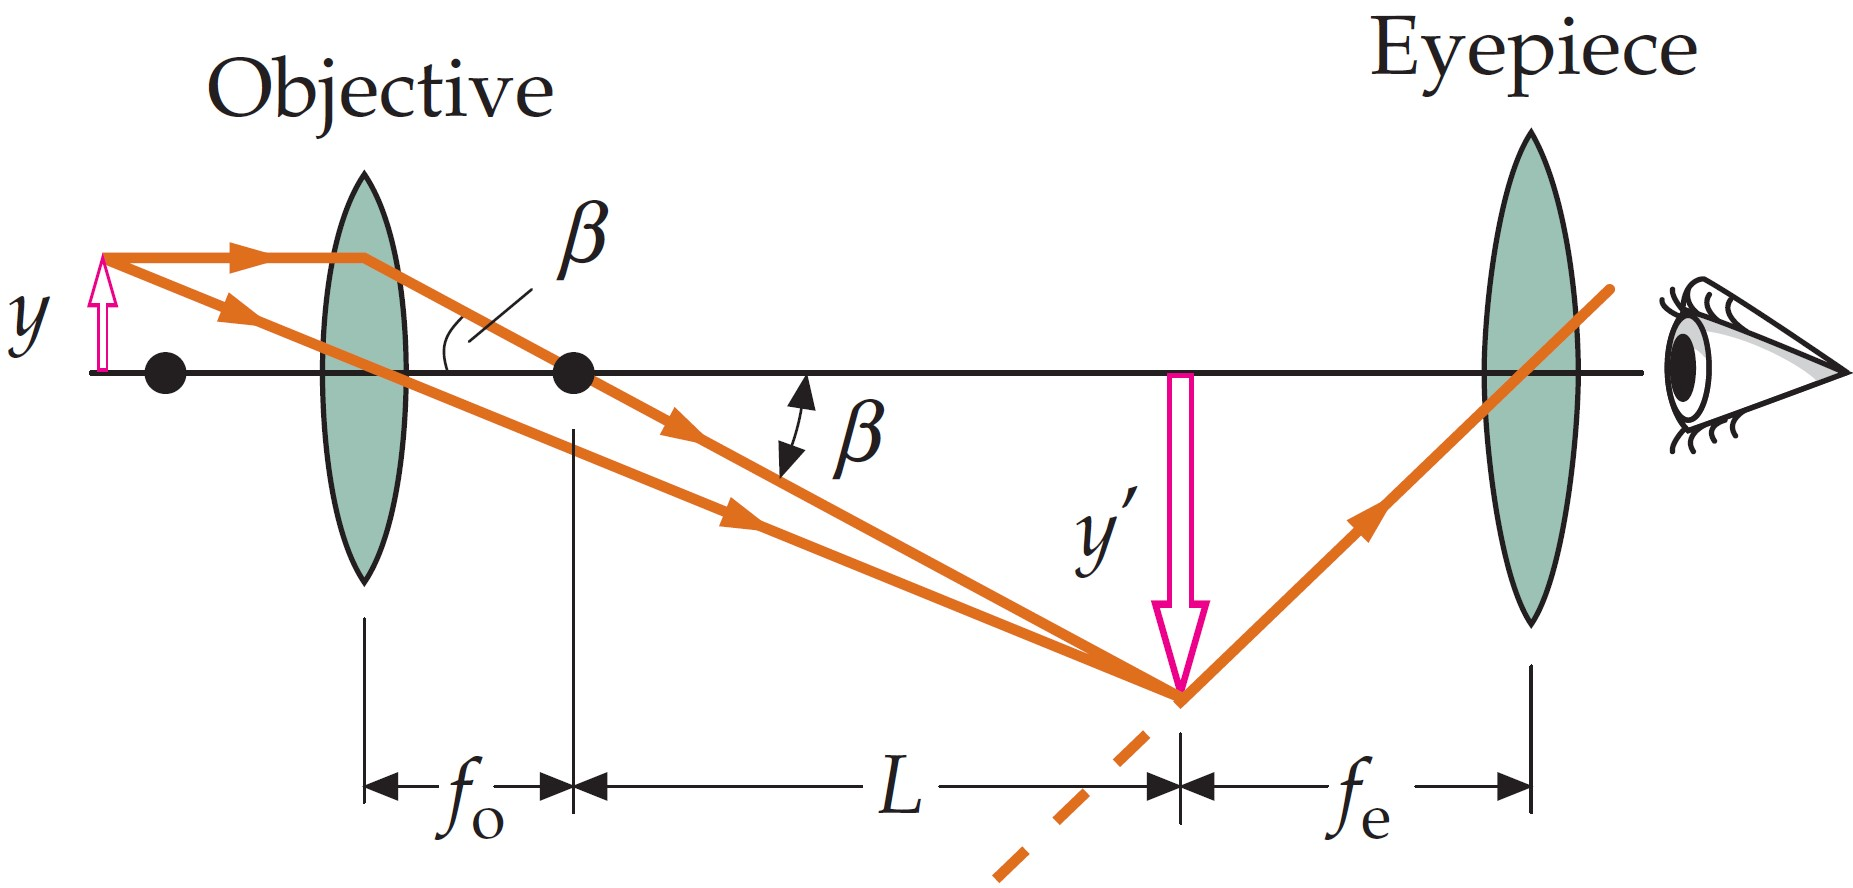
\includegraphics[width=\linewidth]{Physics/1st/Waves_and_optics/Images/micro.jpg}
  %   \captionof{figure}{Microscopi compost per dues lents convergents: un objectiu (amb focal curta) i un ocular (lent d'augment). L'objectiu forma una imatge augmentada $y'$, de l'objecte $y$, real i invertida que podem observar a través de l'ocular.}
  % \end{minipage}
  % Augment total: $$M=M_{\text{obj}}M_{\text{ocu}}=-\frac{L}{f_{\text{o}}}\frac{25\text{ cm}}{f_{\text{e}}}$$
  % Telescopi astronòmic:\newline
  % \begin{minipage}{\linewidth}
  %   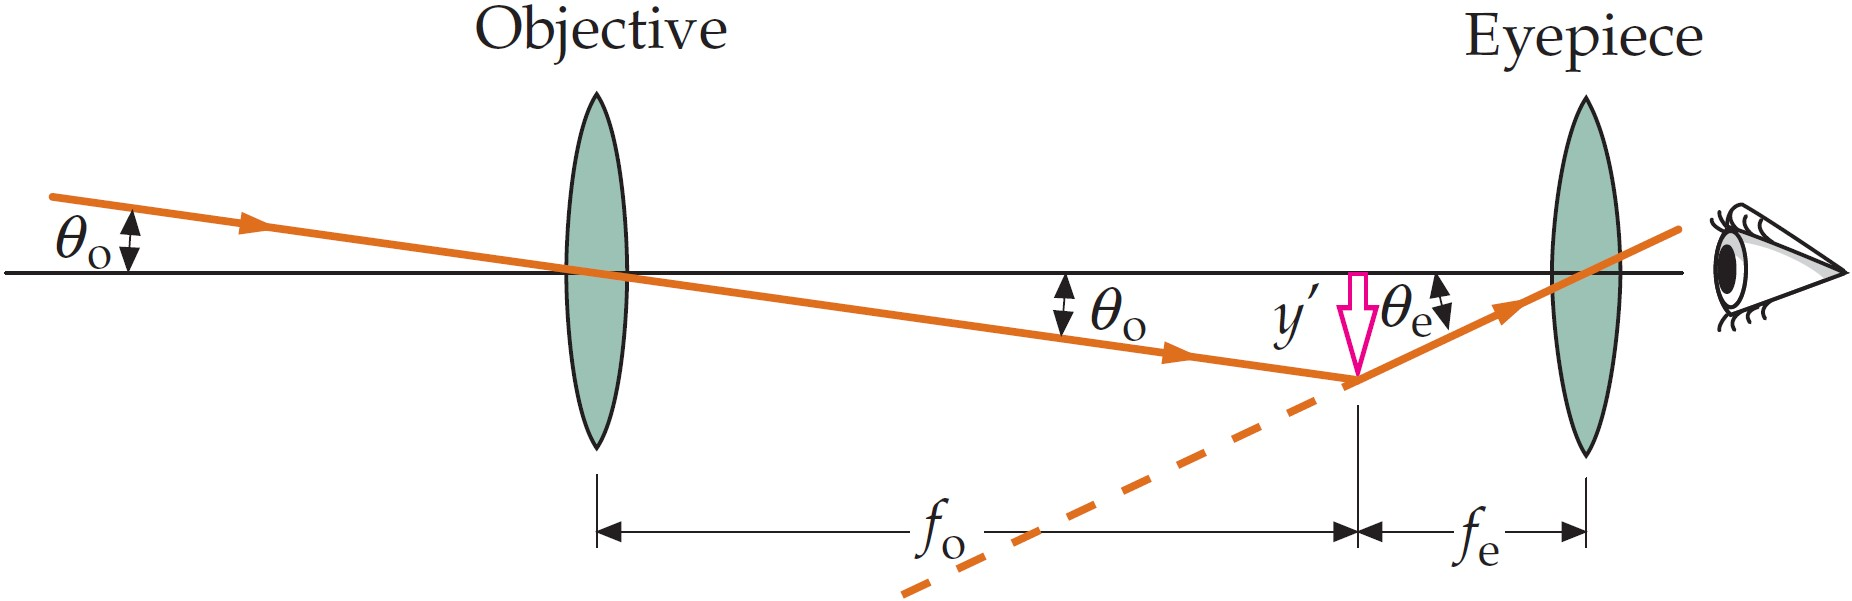
\includegraphics[width=\linewidth]{Physics/1st/Waves_and_optics/Images/tel.jpg}
  %   \captionof{figure}{Telescopi astronòmic compost per dues lents convergents: un objectiu (amb focal llarga) i un ocular (lent d'augment). L'objectiu forma una imatge molt més petita que l'objecte, però molt a prop.}
  % \end{minipage}
  % Poder amplificador del telescopi: $$M=\frac{\theta_\text{e}}{\theta_\text{o}}=\frac{f_{\text{o}}}{f_{\text{e}}}$$
  % \subsection{Interferències i difracció}
  % Fórmula fonamental de les interferències: Donades dues ones amb intensitats $I_1,I_2$ i diferència de fase $\delta$: $$I_T=I_1+I_2+2\sqrt{I_1I_2}\cos\delta$$
  % {\footnotesize on $\delta$ pot dependre, per exemple, de la diferència de camins ($r_2,r_1$), de manera que $\delta=2\pi\Delta r/\lambda$, o del canvi de fase en la reflexió en una superfície.}\newline
  % Tipus d'interferències:
  % \begin{itemize}
  %   \item Interferència per divisió d'amplitud:
  %         \begin{itemize}
  %           \item Làmines primes:\newline
  %                 \begin{minipage}{\linewidth}
  %                   \centering 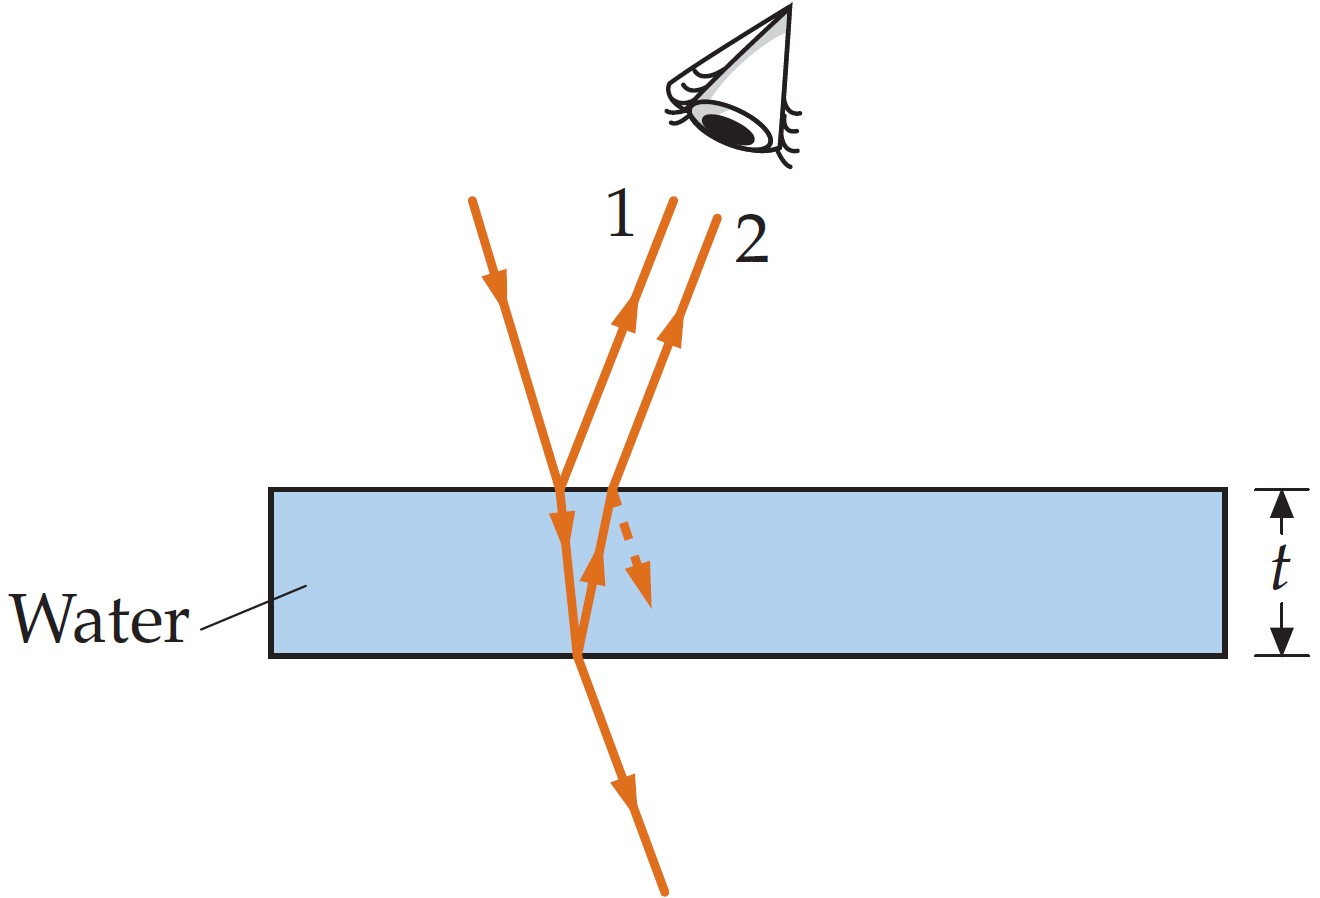
\includegraphics[width=\linewidth]{Physics/1st/Waves_and_optics/Images/lamprim.jpg}
  %                   \captionof{figure}{Làmina prima. Apareixen taques de color, per exemple en bombolles de sabó o taques d'oli.}
  %                 \end{minipage}
  %                 Si estem a prop de la incidència normal, els dos feixos se superposen amb una diferència de fase $\delta$: $$\delta=\frac{2\pi}{\lambda}2nd+\pi$$ {\footnotesize on el primer terme correspon al canvi de fase per la diferència de camins i el segon terme al canvi de fase per a la reflexió interna.}
  %           \item Anells de Newton:\newline
  %                 \begin{minipage}{\linewidth}
  %                   \centering 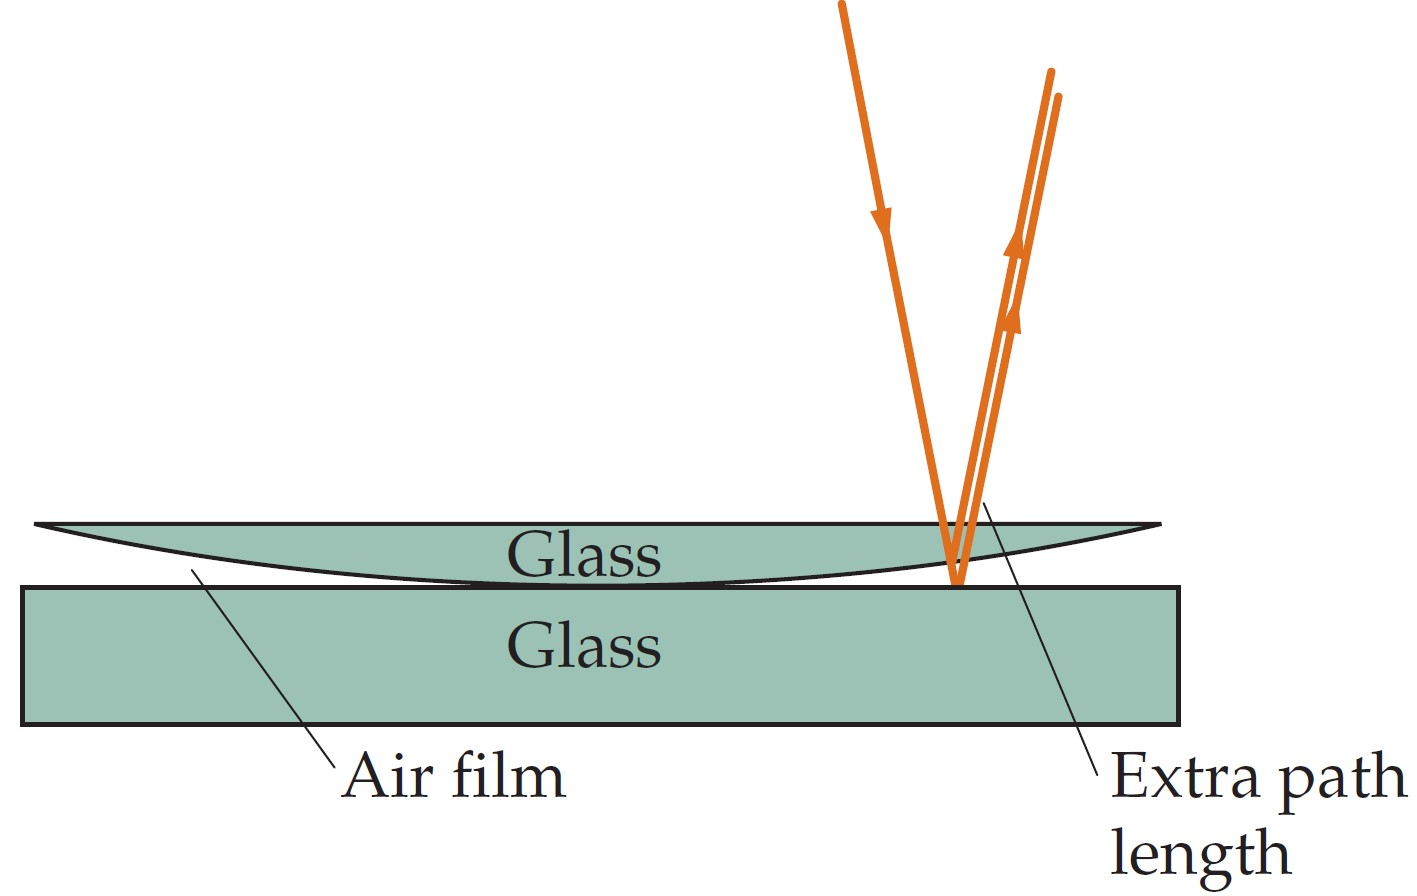
\includegraphics[width=\linewidth]{Physics/1st/Waves_and_optics/Images/newton.jpg}
  %                   \captionof{figure}{Anells de Newton. Ara el desfasament depèn del radi. És per això que observem un patró circular d'interferències.}
  %                 \end{minipage}
  %           \item Franges de Fizeau:\newline
  %                 \begin{minipage}{\linewidth}
  %                   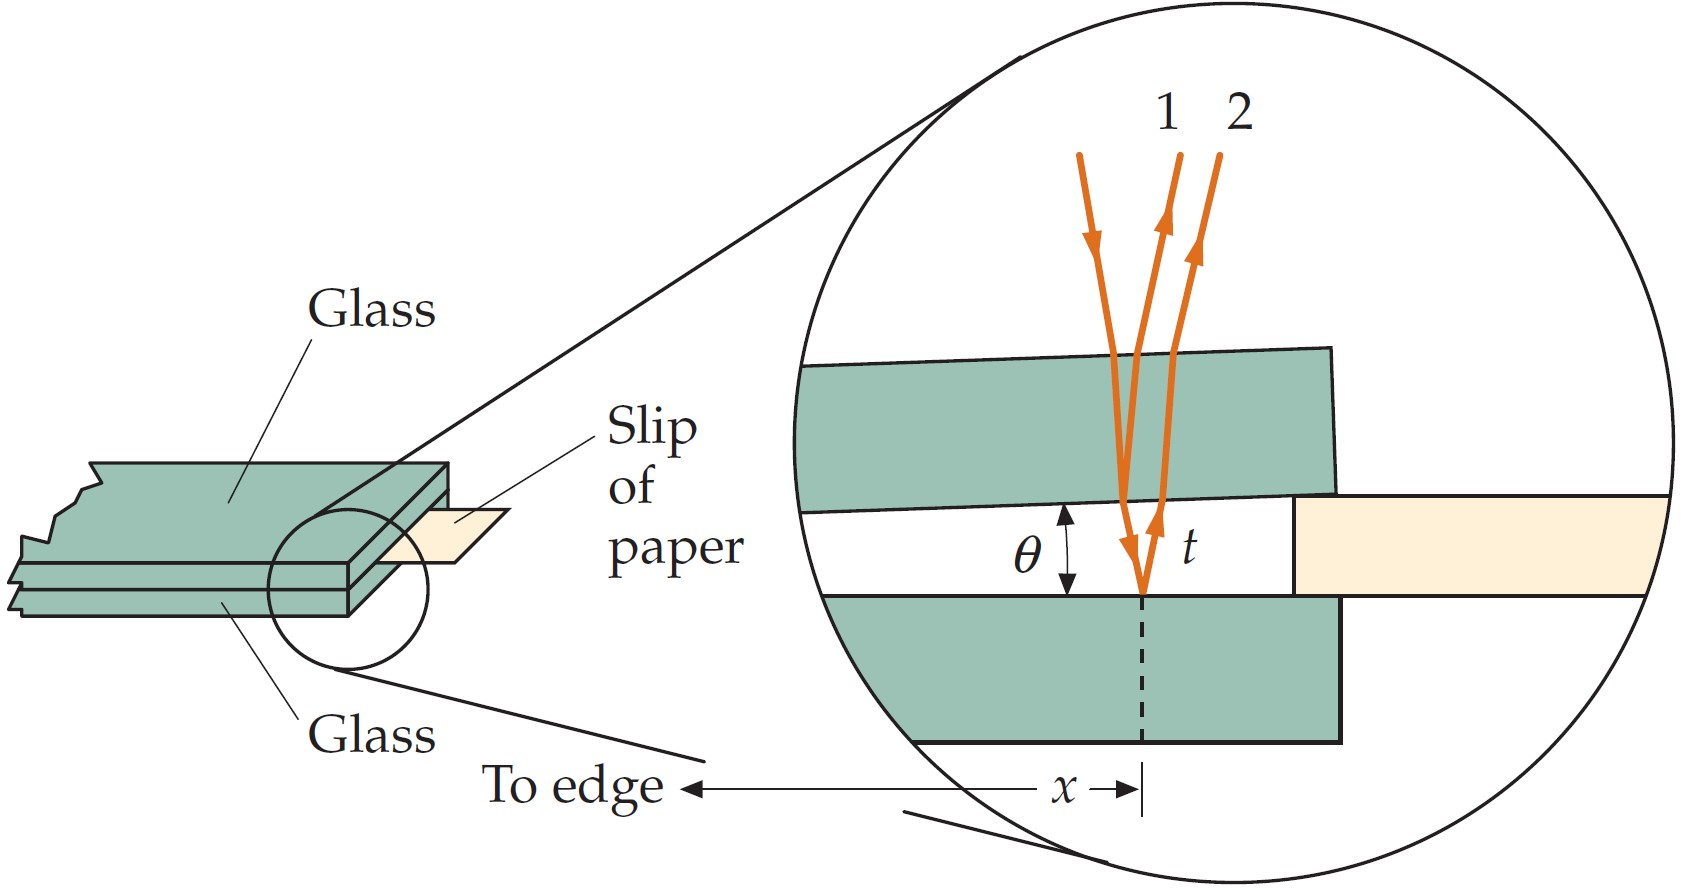
\includegraphics[width=\linewidth]{Physics/1st/Waves_and_optics/Images/fizeau.jpg}
  %                   \captionof{figure}{}
  %                 \end{minipage}
  %           \item Interferòmetre Michelson: $$I_T=I_0\cos^2(\delta/2)$$ {\footnotesize on $I_0$ és la intensitat inicial de la llum.}\newline
  %                 Si la font és puntual, es formen anells d'interferència i $$\delta=\frac{2\pi}{\lambda}(d_1-d_2)2n_{\text{aire}}\cos\alpha$$ {\footnotesize on $d_1,d_2$ són les distàncies dels miralls 1 i 2, respectivament, a la làmina semitransparent i $\alpha$ és l'angle respecte l'horitzontal amb què incideix la llum.}
  %           \item Variants d'interferòmetre:
  %                 \begin{itemize}
  %                   \item Mach-Zehnder:\newline
  %                         \begin{minipage}{\linewidth}
  %                           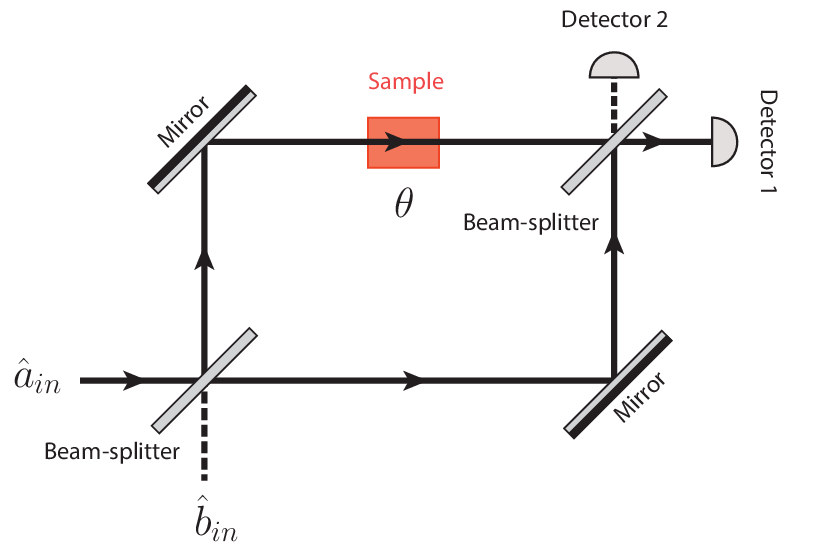
\includegraphics[width=\linewidth]{Physics/1st/Waves_and_optics/Images/zehnder.png}
  %                           \captionof{figure}{}
  %                         \end{minipage}
  %                   \item Fabry-Pérot:\newline
  %                         \begin{minipage}{\linewidth}
  %                           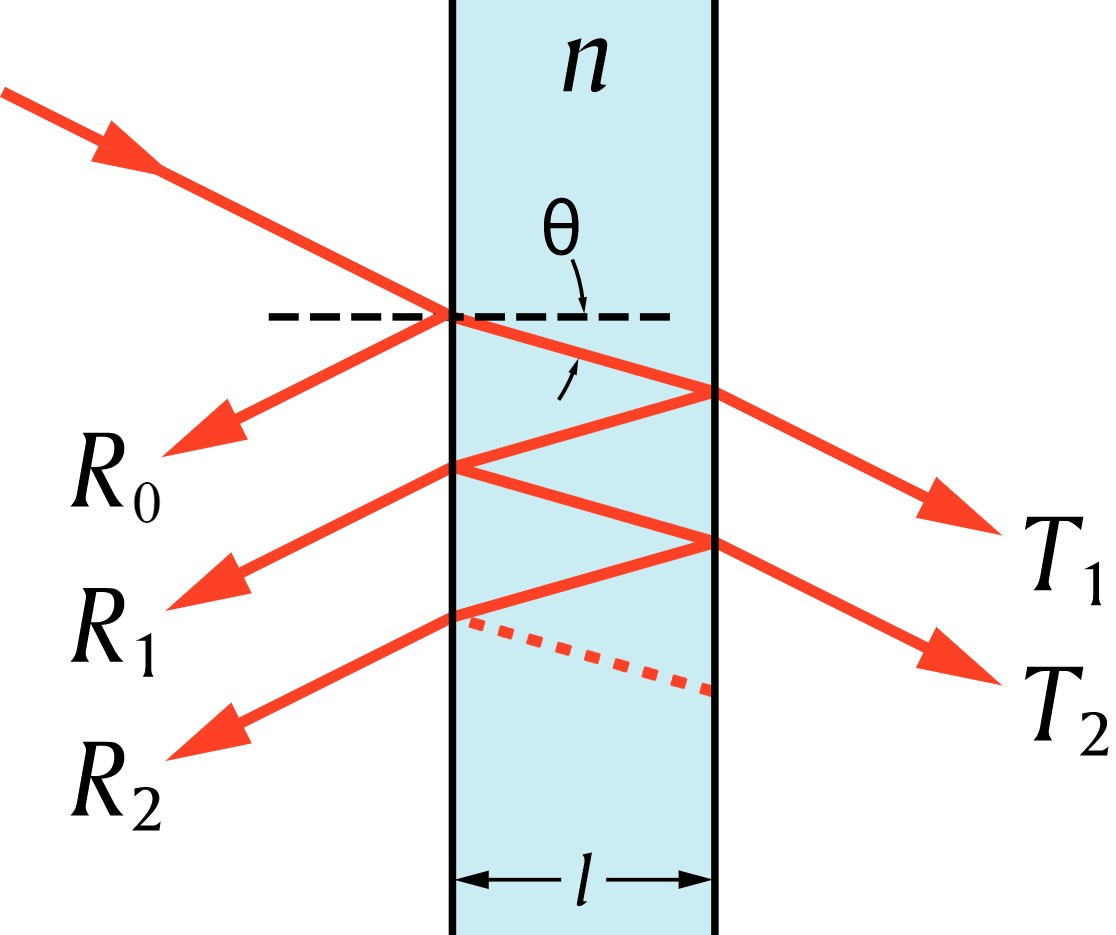
\includegraphics[width=\linewidth]{Physics/1st/Waves_and_optics/Images/fabry.jpg}
  %                           \captionof{figure}{}
  %                         \end{minipage}
  %                 \end{itemize}
  %         \end{itemize}
  %   \item Interferència per divisió de front d'ona:
  %         \begin{itemize}
  %           \item Doble escletxa de Young:\newline
  %                 \begin{minipage}{\linewidth}
  %                   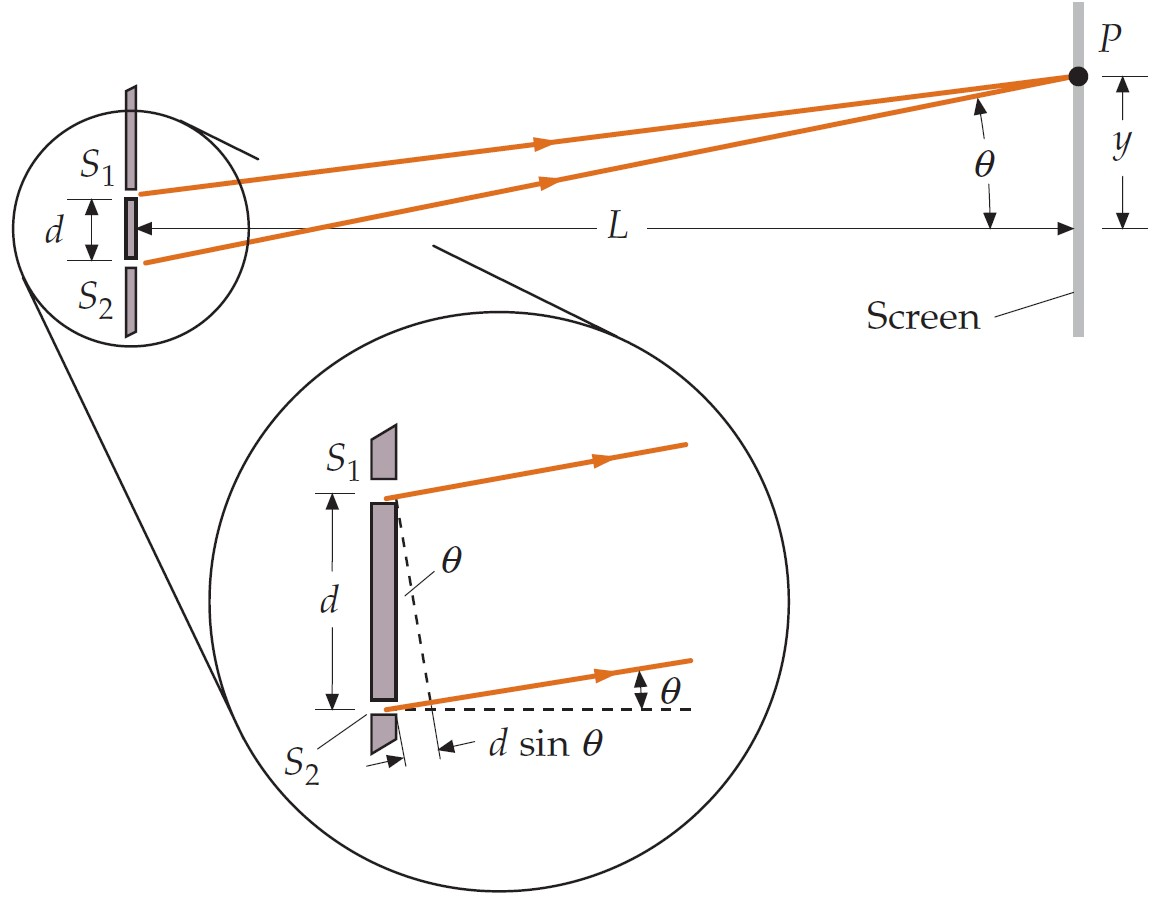
\includegraphics[width=\linewidth]{Physics/1st/Waves_and_optics/Images/young.jpg}
  %                   \captionof{figure}{Doble escletxa de Young. Considerarem $L>>d$ i $L>>y$.}
  %                 \end{minipage}
  %                 Màxims d'interferència: $$d\sin\theta=m\lambda$${\footnotesize on $m\in\NN$.}\newline
  %                 Mínims d'interferència: $$d\sin\theta=(m+1/2)\lambda$$ {\footnotesize on $m\in\NN$.}\newline
  %                 Franges equidistants separades: $$\Delta y=\frac{\lambda L}{d}$$
  %                 Diferència de fase en el punt P:
  %                 $$\delta=\frac{2\pi}{\lambda}d\sin\theta$$
  %                 Intensitat total: $$I_T=4I_0\cos^2(\delta/2)$$
  %           \item Variants de la doble escletxa de Young:
  %                 \begin{itemize}
  %                   \item Mirall de Lloyd:\newline
  %                         \begin{minipage}{\linewidth}
  %                           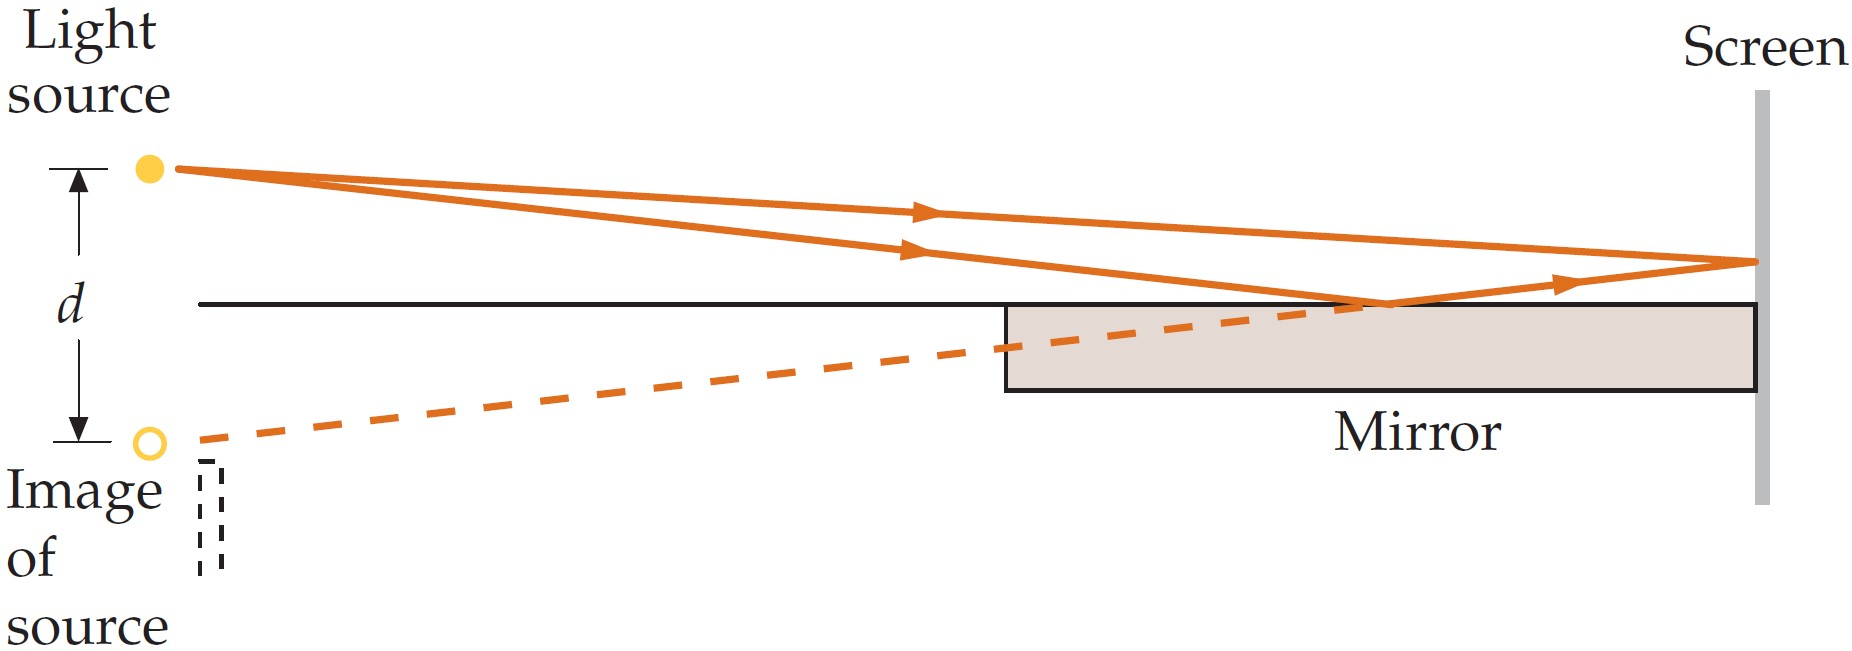
\includegraphics[width=\linewidth]{Physics/1st/Waves_and_optics/Images/lloyd.jpg}
  %                           \captionof{figure}{}
  %                         \end{minipage}
  %                         $$\delta=\frac{2\pi}{\lambda}d\sin\theta+\pi$$
  %                   \item Biprisma de Fresnel: Hi ha una zona concreta d'in\-ter\-fe\-rèn\-cia.
  %                 \end{itemize}
  %           \item Difracció d'una escletxa d'am\-pla\-da $a$:\newline
  %                 \begin{minipage}{\linewidth}
  %                   \includegraphics[width=\linewidth]{Physics/1st/Waves_and_optics/Images/dif1.jpg}
  %                   \captionof{figure}{Difracció d'una escletxa. A la dreta es representa el gràfic de la intensitat en funció de $\sin\theta$.}
  %                 \end{minipage}
  %                 Mínim d'interferència:
  %                 $$\sin\theta=m\frac{\lambda}{a}$$ {\footnotesize on $m\in\NN$}.\newline Si $L>>y$ i $L>>a$, la integral de Kirchhoff ens dona la intensitat de la llum que tindrem: $$I(\theta)=I_0\frac{\sin^2\beta}{\beta^2}$$ {\footnotesize on $\beta=\frac{2\pi}{\lambda}\frac{a}{2}\sin\theta$.}
  %           \item Difracció de dues escletxes d'am\-pla\-da $a$ i separació $d$:\newline
  %                 Intensitat: $$I(\theta)=4I_0\frac{\sin^2\beta}{\beta^2}\cos^2(\delta/2)$$ {\footnotesize on $\beta=\frac{2\pi}{\lambda}\frac{a}{2}\sin\theta$ i $\frac{\delta}{2}=\frac{2\pi}{\lambda}\frac{d}{2}\sin\theta$.}\newline      \begin{minipage}{\linewidth}
  %                   \includegraphics[width=\linewidth]{Physics/1st/Waves_and_optics/Images/dif2.jpg}
  %                   \captionof{figure}{Gràfic d'intensitat en funció de $\sin\theta$ de la difracció de dues escletxes. Observem que la difracció d'una escletxa modula el $\cos^2(\delta/2)$ que re\-pre\-sen\-ta la interferència entre dues ones.}
  %                 \end{minipage}
  %           \item Difracció de $N$ escletxes i\-dèn\-ti\-ques d'amplada $a$ i separades una distància $d$:\newline
  %                 Intensitat: $$I(\theta)=I_0\frac{\sin^2\beta}{\beta^2}\frac{\sin^2(N\delta/2)}{\sin^2(\delta/2)}$$ {\footnotesize on $\beta=\frac{2\pi}{\lambda}\frac{a}{2}\sin\theta$ i $\frac{\delta}{2}=\frac{2\pi}{\lambda}\frac{d}{2}\sin\theta$.}\newline
  %                 \begin{minipage}{\linewidth}
  %                   \includegraphics[width=\linewidth]{Physics/1st/Waves_and_optics/Images/difn.png}
  %                   \captionof{figure}{ Difracció de $N$ escletxes en el cas que $N=5$. En aquesta gràfica tenim els mínims de difracció per $\sin\theta=m\frac{\lambda}{a}$, $m\in\ZZ\setminus\{0\}$ i màxims $\sin\theta=m\frac{\lambda}{d}$, $m\in\ZZ$. Entre dos màxims principals hi ha $N-2$ màxims secundaris i $N-1$ mínims que corresponen quan $\sin\theta=m\frac{\lambda}{Nd}$, $m\in\ZZ\setminus\{0\}$ i $m\ne kN$, $k\in\ZZ$. }
  %                 \end{minipage}
  %           \item Difracció de Fraunhofer i de Fresnel:
  %                 \begin{itemize}
  %                   \item de Fraunhofer: si la pantalla és molt lluny de l'obertura.
  %                   \item de Fresnel: si la pantalla és a prop de l'obertura.
  %                 \end{itemize}
  %                 \begin{minipage}{\linewidth}
  %                   \includegraphics[width=10cm]{Physics/1st/Waves_and_optics/Images/fraun.jpg}
  %                   \captionof{figure}{Gràfic de la intensitat a mesura que acostem la pantalla a l'obertura.}
  %                 \end{minipage}
  %           \item Difracció i resolució:\newline
  %                 \begin{minipage}{\linewidth}
  %                   \includegraphics[width=\linewidth]{Physics/1st/Waves_and_optics/Images/reso.jpg}
  %                   \captionof{figure}{Interferència de dues fonts puntuals.}
  %                   $$\sin\theta=1,22\frac{\lambda}{D}\approx\theta$$
  %                   Si volem que les dues taques imatges estiguin separades $\rightarrow$
  %                   Criteri de resolució de Rayleigh: $$\alpha>\theta\approx1,22\frac{\lambda}{D}$$
  %                 \end{minipage}
  %           \item Xarxes de difracció: Moltes escletxes ($N$) petites idèntiques separades una distància $d$.\newline
  %                 Equació de la xarxa de difracció (màxims d'interferència): $$d\sin\theta=m\lambda$$ {\footnotesize on $m\in\ZZ$.}\newline
  %                 Els màxims secundaris són molt petits i, per tant, els podem ne\-gli\-gir.\newline
  %                 Amplada dels pics: $$\Delta(\sin\theta)=\frac{\lambda}{Nd}$$
  %                 Poder de resolució $\mathcal{R}$: $$\mathcal{R}=\frac{\lambda}{\Delta\lambda}=Nm$$ {\footnotesize on $\Delta\lambda=\lambda_1-\lambda_2$ i $m\in\ZZ$.}\newline
  %                 Els pics de dos $\lambda$'s estan separats si $\mathcal{R}\leq Nm$.
  %         \end{itemize}
  % \end{itemize}
\end{multicols}
\end{document}